% TODO: Write about states and density matrices
% TODO: Add appendix about the JC interaction Hamiltonian and sisspertion
% TODO: Add appendix about quantum optics, coherent states, fock states

\documentclass[english, a4paper, 12pt, twoside]{article} 

\usepackage{etex}
\usepackage[table,xcdraw]{xcolor}
\usepackage[utf8]{inputenc}
\usepackage{appendix}
\usepackage{amsfonts}
\usepackage{textcomp}
\usepackage[T1]{fontenc, url}
\usepackage{titlesec}
\setcounter{secnumdepth}{4}
\usepackage{multirow}
\usepackage{minted} % Code highlighting
\usepackage{adjustbox}
\usepackage{gensymb}
\usepackage{graphicx}
\usepackage{amsmath, amssymb, amsthm} % Mathematical packages
\usepackage{parskip} % Removing indenting in new paragraphs
\urlstyle{sf}
\usepackage{color}
\usepackage{subcaption} 
\usepackage{appendix}
\usepackage{chngcntr} % needed for correct table numbering
\counterwithin{table}{section} % numbering of tables 
\counterwithin{figure}{section} % numbering of figures
\numberwithin{equation}{section} % numbering of equations
\hyphenpenalty=100000 % preventing splitting of words
\sloppy 
\raggedbottom 
\usepackage{xparse,nameref}
\usepackage[bottom]{footmisc} % Fotnotes are fixed to bottom of page
\usepackage{lipsum} % For genereating dummy text

% My Packages
\usepackage{dirtytalk}
\usepackage{tikz,tkz-graph,tkz-berge}
\usepackage{listings}
\usepackage{physics}
% \usepackage[raggedright]{titlesec}


\usepackage{hyperref}
\hypersetup{
    colorlinks,
    citecolor=black,
    filecolor=black,
    linkcolor=black,
    urlcolor=black
}

\usepackage[margin=2.54cm]{geometry} % sets margins for the document
\usepackage{setspace}
\linespread{1.5} % line spread for the document
\usepackage{microtype}

% ----- Sections -----
\titleformat*{\section}{\LARGE\bfseries} % \section heading
\titleformat*{\subsection}{\Large\bfseries} % \subsection heading
\titleformat*{\subsubsection}{\large\bfseries} % \subsubsection heading
% next three lines creates the \paragraph command with correct heading 
\titleformat{\paragraph}
{\normalfont\normalsize\bfseries}{\theparagraph}{1em}{}
\titlespacing*{\paragraph}
{0pt}{3.25ex plus 1ex minus .2ex}{1.5ex plus .2ex}


% ----- Figures and tables ----- 
\usepackage{fancyhdr}
\usepackage{subfiles}
\usepackage{array}
\usepackage[rightcaption]{sidecap}
\usepackage{wrapfig}
\usepackage{float}
\usepackage[labelfont=bf]{caption} % bold text for captions
\usepackage[para]{threeparttable} % fancy tables, check these before you use them
\usepackage{url}
\usepackage[table,xcdraw]{xcolor}
\usepackage{makecell}
\usepackage{hhline}


% ----- Sources -----
\usepackage{natbib}
\bibliographystyle{apa} % citation and reference list style
\def\biblio{\clearpage\bibliographystyle{apa}\bibliography{References.bib}} % defines the \biblio command used for referencing in subfiles - DO NOT CHANGE

% ----- Header and footer -----
% \pagestyle{fancy}
% \fancyhead[R]{\thepage} % page number on right for odd pages and left for even pages in the header
% \fancyhead[L]{\nouppercase{\rightmark}} % chapter name and number on the right for even pages and left for

% ----- Header and footer -----
\pagestyle{fancy}
\fancyhead[RE,LO]{\thepage} % page number on right for odd pages and left for even pages in the header
\fancyhead[RO,LE]{\nouppercase{\rightmark}} % chapter name and number on the right for even pages and left odd pages in the header
%\renewcommand{\headrulewidth}{0pt} % sets thickness of header line
\fancyfoot{} % removes page number on bottom of page

% ----- Header of the frontpage ----- 
\fancypagestyle{frontpage}{
	\fancyhf{}
	\renewcommand{\headrulewidth}{0pt}
	\renewcommand{\footrulewidth}{0pt}
	\vspace*{1\baselineskip}
	
% 	\fancyhead[C]{Bachelor Project for The Open University of Israel
% 	\linebreak       Done at The Weizmann Institute of Science\vspace*{5\baselineskip}}
% 	\fancyhead[L]{ 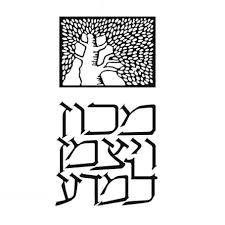
\includegraphics[width=1.2in]{Logo.png}}
% 	\fancyhead[R]{ 
\includegraphics[width=1.2in]{OpenLogo.jpg}}
}

%-----------------------------------------------------

%\title{Controlling a Superconducting Quantum Computer}
%\author{Daniel Cohen Hillel}
%\date{}
\setlength{\headheight}{15pt}

\begin{document}

\def\biblio{} % resets the biblio command, if not here a new reference list will be produced after every chapter
\begin{titlepage}
	
	\newgeometry{top=1 in, bottom=1 in, left=1 in, right= 1 in} 
	
	\thispagestyle{frontpage}
	
	\begin{center}
		
		\vspace*{6\baselineskip}
	
		
		{\Large \textbf{Controlling a Superconducting Quantum Computer\\}}
		
        \vspace*{1,5\baselineskip}

		\large{\textbf{Daniel Cohen Hillel}}\\
		\large{\textbf{Supervisor: Dr. Serge Rosenblum}}\\
		
		\vspace{1,5\baselineskip}
		
		\large{Advanced Project in Physics A (20382)}\\
		\large{The Open University of Israel}\\
		
		\vspace{1,5\baselineskip}
		\large{The Weizmann Institute}\\

	\end{center}
	
\end{titlepage}


\restoregeometry % restores the margins after frontpage
%\nocite{*} % uncomment if you want all sources to be printed in the reference list, including the ones which are not cited in the text 

\pagenumbering{gobble} % suppress page numbering
\thispagestyle{plain} % suppress header

%\maketitle

\newpage

\tableofcontents

\newpage
\pagenumbering{arabic}
\begin{abstract}
   Quantum computing presents many challenges, we're going to try to tackle one of them, Quantum Optimal Control. How do we control the quantum computer? What do you need to send to make what you want happen? How do you physically build control the transmission of the control pulses and what the pulses even look like? These are all question we are going to try to answer throughout this project.\newline\newline
   The project starts with an introduction to quantum computing. This is the basic of quantum computing and is only meant for readers who have no knowledge of quantum computing. Concepts such as the qubit and operations are introduced there.\newline\newline
   In the section chapter we define the system and characterize it. We use quantum optics and the Jaynes-Cumming model to characterize the system. This is where the bulk of the pure physics is done.\newline\newline
   The third chapter is the main interest of this project, quantum optimal control and the GRAPE algorithm. In this chapter we show how can you use the system characterization we made in chapter 2 to find the pulses you need to send to control the quantum computer as you want.\newline\newline
   The fourth and last chapter talks about the physical implementation of the transmission of the pulses we found in the previous chapter. We show how the entire system is connected, from the AWG\footnote{Arbitrary Waveform Generator, read the chapter to learn more} to the actual qubits. We discuss the challenges of creating the pulses and how to solve these problems.\newline\newline
   All the codes used in and created for this project, results, and references are available at\newline
   \texttt{https://github.com/DanielCohenHillel/Controlling-a-Superconducting-Quantum-Computer}
   
\end{abstract}
\newpage
\section{Introduction}
\subsection{What is a Quantum Computer?}
We'll assume the reader is familiar with the basics of computing and quantum mechanics, here's a brief overview. \newline
 A classical computer is, essentially, a calculator, not of "Regular" numbers but of \textit{binary numbers}. % TODO: Maybe add some further readings about binary numbers
 A \textit{binary digit}("\textit{bit}" from now on) can be in one of two states, usually represented by 0 and 1. We can use \textit{logic gates} to control and manipulate bits to do all kinds of calculations. These are the building blocks of the classical computer, with the ability to do calculation on bits, and the ability to store bits in the memory we are able to construct a computer.
 
So what is a quantum computer then? Well, if the classical computer uses bits to do calculations, a quantum computer uses \textit{quantum bits}("\textit{qubits}" from now on) for it's calculations. A qubit, much the same as a bit, has 2 states, a 0 state and a 1 state(notated $\ket{0}$ and $\ket{1}$ for reasons we'll see later), the difference between bits and qubits is that a qubit can be in a \textit{superposition} of the 2 states, we can use this property to our advantage to create new type of computation, \textit{quantum computation}.

\subsection{Algorithms and Further motivation}
 \begin{quotation}
  \say{Nature isn't classical, dammit, and if you want to make a simulation of nature, you'd better make it quantum mechanical, and by golly it's a wonderful problem, because it doesn't look so easy.}
 \end{quotation}
\centerline{- Richard Feynman}
Quantum computation is a cool idea and all, but it becomes much more interesting when you think of the possibilities of its uses. From simulation of drugs for developments of new cures to unbreakable encryption, quantum computing promises a lot. 

One of the most famous algorithms in quantum computing is \textit{Shor's algorithm}. Shor's algorithm is a quantum algorithm to factor large numbers, in classical computing the best way to factor a number is to try all the numbers smaller then it and check if they devise the number. This is a really slow way to do it and basically impossible for computers to do. For this reason, almost everything is encrypted in a way that uses the fact that it is really hard to factor large numbers, to decrypt information you're not supposed to see, you need to factor a really big number\footnote{This is called RSA encryption}. With classical computers this is a nearly impossible problem, it's exponential in time, meaning that if we increase the size of the number that we need to factor by just a little bit, it becomes much, much harder to solve. Shor's algorithm, on the other hand, uses the power of quantum computing to solve this problem in logarithmic time!\footnote{The actual complexity is more detailed then this but it is meant to show the rough idea} Even if you increase the size of the number that you want to factor by huge amounts the time it would take for Shor's algorithm to factor the number will barley change! This means that in most cases, a classical computer could take thousands of years to solve a problem that may take only a couple of seconds on a quantum computer. 

While Shor's algorithm is a great example of the power of quantum computers, and it is also probably the most famous quantum algorithm, Shor's algorithm isn't the most interesting example, decrypting messages and breaking the world's cryptography isn't really a good motivator to try to create quantum computers. Let's look at a more useful, optimistic algorithm, \textit{Grover's Algorithm}.

Grover's algorithm is a quantum algorithm that finds the unique input to a black box function that produces a particular output value, using just $o(\sqrt {N})$ evaluations of the function, where $N$ is the size of the function's domain. For a classical algorithm to do this it would take $o(N)$ evaluations, there's a polynomial improvement. Roughly speaking, given function $y = f(x)$ Grover's algorithm finds $x$ when given a specific $y$. This algorithm could be used to search in databases much faster then with a classical computer, something that is extremely important in our modern world.

There are many more quantum algorithms that were developed in the last several decades, and even more algorithms that have yet to be developed that might have amazing applications in the future. The applications of quantum computers are endless and we've barely touched the surface of quantum algorithms.

\subsection{Qubits and Quantum Gates}
Mathematically, we think of qubits as 2-dimensional vectors, where the first term corresponds to the $\ket{0}$ state and the second term corresponds to the $\ket{1}$ state, so a qubit in a state $\frac{1}{\sqrt{2}} \ket{0} + \frac{1}{\sqrt{2}} \ket{1}$ can be represented as
\[
\begin{pmatrix}
    \frac{1}{\sqrt{2}} \\
    \frac{1}{\sqrt{2}} 
\end{pmatrix} = \frac{1}{\sqrt{2}} \ket{0} + \frac{1}{\sqrt{2}} \ket{1}
\]
The value of each state is correlated to the probability of the qubit to be in that state. The probability is given by the absolute value of that state squared
\[
    P(\ket{\psi}) = \abs{\ket{\psi}}^2
\]
In the example I just gave, the qubit has a $50\%$ chance to be in the $\ket{0}$ state and a $50\%$ chance to be in the $\ket{1}$ state.

In this world of qubits as vectors, we think of logic gates, known as \textit{quantum gates}, as matrices\footnote{Under the constraint that the matrices are unitary}, and when the qubit goes through the logic gate, the result is multiplying the matrix by the qubit. An example for one of the simplest logic gates we have in classical computing, the NOT gate, a quantum implementation of this gate takes $\ket{0}$ to $\ket{1}$ and $\ket{1}$ to $\ket{0}$), the matrix that achieves this is 
\[
\begin{pmatrix}
    0 & 1 \\
    1 & 0
\end{pmatrix}
\]
Known as $\hat{\sigma}_x$(Pauli matrix $X$). As a simple example to see how this works, if we input $\ket{0}$ into the NOT quantum gate, we get as a result
\[
NOT \ket{0} = 
\begin{pmatrix}
    0 & 1 \\
    1 & 0
\end{pmatrix}
\begin{pmatrix}
    1 \\
    0
\end{pmatrix} = 
\begin{pmatrix}
    0 \\
    1
\end{pmatrix} = \ket{1}
\]
As we expected, NOT $\ket{0}$ is $\ket{1}$. There are many more 1-qubit quantum gates we can think of, while in classical computing we only have 4 possible logic gates on a single bit, there are infinite  1-qubit operations on a quantum computer.

The last thing we need to know to understand the basic of quantum computing, is how to represent multiple qubits. If we have several of qubits in our system, we think of all the qubits together as one vector that is the \textit{tensor product}\footnote{Represented as a Kronecker product for the dimensions sake} of all the qubits. Lets say we have a $\ket{0}$ and $\ket{1}$ qubits in our system, we represent that by $\ket{01}$ and it is equal to
\[\ket{01} = \ket{0} \otimes \ket{1} =
\begin{pmatrix}
    0 \\
    1 \\
    0 \\
    0
\end{pmatrix}\]
A quantum gate on multiple qubits is simply a larger matrix.

The tensor product of N qubits has $2^N$ coefficients! This is yet another clue of the power that quantum computers have compared to classical computers. 

Now that we have the basic tools of quantum computing, we can use them to get motivation for the amazing things quantum computers can do

\subsection{Superconducting Quantum Computers}  % TODO: Maybe put this under the "Controlling a superconducting quantum computer" chapter?
The physical implementation of the qubit itself isn't to subject of this project but we still take a look for a bit on how would you implement such a thing. A problem we have to face when making a quantum computer is what physical phenomena would be the qubit, we need some sort of two level system that we can easily measure and manipulate, while also staying coherent\footnote{Coherence is a big subject, you can think of it as a fancy way of saying that the qubit still holds information without being corrupted. This is the main problem facing quantum computing right now} and usable. For classical computers we already have this figured out for years, a bit is a voltage on a wire, 1 is one there is voltage on the wire and 0 if there's none, simple. For a quantum computer this is much more complicated, there are many quantum phenomena we can use as our qubit, such as the energy level of an atom, the spin of an electron, the polarization of photons and so on. It is not so obvious what should be the physical realisation of the qubit. This project is about a \textit{superconducting} quantum computer, with superconducting  qubits.

Superconducting qubits are microwave circuits in which the cooper-pair condensate effectively behaves as a one-dimensional quantized particle. By inserting Josephson junctions, the circuit can be made nonlinear, allowing us to isolate the qubit from higher-energy levels and treat it as a two  level system(instead of the many level system that it really is).

This topic is covered in appendix \ref{appen:LC}, refer there for any additional information, preferably read appendix \ref{appen:LC} after reading chapter \ref{chap:quantum-optics}.
% % TODO: This need to be built from the ground up and can't be all by the way-y. Need to ask Serge and read about superconductors a bit, look into BCS theory, Need to explain much on superconductors and cooper pairs
% Since superconductors are way out of the scope of this project, we can still talk about some of their benefits. The main benefit of superconducting qubits is that they are realized through electrical connections, instead of needing to do some measurement on an atom or photon, you can simply(well, not that simply) connect them to a circuit. More then that, they interact with the electromagnetic field in a very predictable way and we can more or less control them pretty easily. And of course, over the years, thanks for classical computing, methods to create really tiny circuits in very large scales are perfected, just think of how many transistors are in the computer you are using the view this file.
% % TODO: This last paragraph needs to be changes and maybe removed completely

\subsection{References and Further Readings}
The main references for this chapter were two great books on quantum information I recommend everyone to read. The first is the well known, \textit{de-facto} book on quantum computation and information. "\textbf{Quantum Computation and Quantum Information}" written by Michael Nielsen and Isaac Chuang also known as "Mike and Ike". This book covers everything.

The other book I used was "\textbf{Quantum Computing for Computer Scientists}" by Mirco A. Mannucci and Noson S. Yanofsky. It has, in my opinion, clearer explanations on the pure mathematical nature of quantum information, although it is not as comprehensive as "Mike and Ike".

\newpage
\section{Quantum Optics} \label{chap:quantum-optics}
In this chapter we'll introduce concepts in \textit{Quantum Optics}. It's important to have at least a little understanding of quantum optics before reading the project. The implementation of quantum computers we discuss in this project has a qubit which is a two level system interacting with light(classical and quantum) inside a cavity. The cavity is some box made out of a conducting material, and inside there are modes of quantized light interacting with the qubit.

This won't be an in depth review of quantum optics and wouldn't even scratch the surface of the subject. If you want a much better introduction the the subject I highly recommend "Introductory Quantum Optics" by Christopher C. Gerry and Peter L. Knight. This chapter will only touch the subjects related and used by the project.

\subsection{Dirac's Method for Canonical Quantization}
Before we dive into anything new, we'll start by going over the method to quantize any oscillating phenomena introduced by Paul Dirac in his 1925 PhD dissertation.

Any system of which we have a classical description can be quantized following a process known as canonical quantization. A classical system can be described by pairs of \textit{canonically conjugate variables}, $(q_j, p_j)$ satisfying the Hamilton equations
\begin{align*}
    &\dot{q_j} =\quad \frac{\partial H}{\partial p_j} \\
    &\dot{p_j} = -\frac{\partial H}{\partial q_j}
\end{align*}
where $q_j$ is called the \textit{canonical coordinate} and $p_j$ is called the \textit{canonically conjugate momentum to the coordinate $q_j$}.

To quantize the system we need to replace the dynamical variables $(q_j, p_j)$ with canonically conjugate operators $(\hat{q_j}, \hat{p_j})$ satisfying the commutation relation $[\hat{q_j}, \hat{p_k}] = i\hbar \delta_{jk}$ and now the Hamiltonian of the system is replaced from the classical Hamiltonian $E = H(q_1,p_1, \dots ,q_j, p_j, \dots)$ to the quantum Hamiltonian $\hat{H} = H(\hat{q_1},\hat{p_1}, \dots ,\hat{q_j}, \hat{p_j}, \dots)$. We know that we can get any physical observable and the time evolution of states from the Hamiltonian using the schr\"{o}dinger equation. If we have the Hamiltonian, we have everything.

I don't want to get too much into the example of the quantum harmonic oscillator because it is expected that the reader is already familiar with it. I'll just mention, that using Dirac's method, when solving the quantum harmonic oscillator we introduce annihilation and creation operators, $\hat{a}$ and $\hat{a}^\dag$ respectively, which are hermitian conjugates of each other, satisfying the commutation relation $[\hat{a}, \hat{a}^\dag] = 1$ meaning they are not observables, but all observables can be expressed with $\hat{a}$ and $\hat{a}^\dag$. $\hat{a}$ and $\hat{a}^\dag$ also have the nice property
\begin{align*}
    &\hat{a}^\dag \ket{n} = \sqrt{n+1}\ket{n+1} \\
    &\hat{a} \ket{n} = \sqrt{n}\ket{n-1} \\
    &\hat{a}\ket{0} = 0
\end{align*}
where $\ket{n}$ is the $n^{th}$ energy level of the system and $\ket{0}$ is the vacuum state. You can think of the annihilation and creating operators, as their name suggest, that they destroy(or reduce by one) and create(or increase by one) the state of the system when applied to a state.

\subsection{The Quantization of the Electromagnetic Field}
\subsubsection{The Homogeneous Electromagnetic Equation}
We'll start from Maxwell's equations, proving one of the most important result of the electromagnetic theory that you've properly encountered before in you classical electromagnetism course.

Maxwell's equations in free space are:
\begin{subequations}
    \label{eq:optim}
    \begin{align}
        &\grad \cdot \textbf{E} = 0 \label{eq:Maxwell-1} \\
        &\grad \cdot \textbf{B} = 0 \label{eq:Maxwell-2}\\
        &\grad \cross \textbf{E} = \frac{\partial\textbf{B}}{\partial t} \label{eq:Maxwell-3}\\
        &\grad \cross \textbf{B} = \mu_0 \epsilon_0 \frac{\partial\textbf{E}}{\partial t} \label{eq:Maxwell-4}
    \end{align}
\end{subequations}
Taking the curl of \ref{eq:Maxwell-3} and \ref{eq:Maxwell-4} we get
\begin{subequations} 
\label{eq:curl-}
    \begin{align}
        &\curl{(\curl{\textbf{E}})} 
        = \curl{(-\frac{\partial \textbf{B}}{\partial t})} 
        = -\frac{\partial}{\partial t}(\curl{\textbf{B}})
        = - \mu_0 \epsilon_0 \frac{\partial^2 E}{\partial t^2} 
        \label{eq:curl-E}\\
        &\curl{(\curl{\textbf{B}})} 
        = \curl{(\mu_0 \epsilon_0 \frac{\partial E}{\partial t})} 
        = \mu_0 \epsilon_0\frac{\partial}{\partial t}(\curl{E}) 
        = - \mu_0 \epsilon_0 \frac{\partial^2 \textbf{B}}{\partial t^2} 
        \label{eq:curl-B}
    \end{align}
\end{subequations}
   
We can use the vector identity
\begin{equation}
    \nabla \times \left( \nabla \times \mathbf{V} \right) = \nabla \left( \nabla \cdot \mathbf{V} \right) - \nabla^2 \mathbf{V}
\end{equation}
And obtain from \ref{eq:curl-E} and \ref{eq:curl-B}
\begin{subequations}
    \begin{align}
        &\nabla(\nabla \cdot \textbf{E}) - \nabla^2 \textbf{E} 
        = -\mu_0\epsilon_0\frac{\partial^2 \textbf{E}}{\partial t^2} \\
        &\nabla(\nabla \cdot \textbf{B}) - \nabla^2 \textbf{B} 
        = -\mu_0\epsilon_0\frac{\partial^2 \textbf{B}}{\partial t^2}
    \end{align}
\end{subequations}
Now, we can use \ref{eq:Maxwell-1} and \ref{eq:Maxwell-2} To cancel the left most term and get
\begin{subequations}
    \begin{align}
        &\nabla^2 \textbf{E} = \mu_0\epsilon_0\frac{\partial^2 \textbf{E}}{\partial t^2}\\
        &\nabla^2 \textbf{B} = \mu_0\epsilon_0\frac{\partial^2 \textbf{B}}{\partial t^2}
    \end{align}
\end{subequations}
Now because we know that $v_{ph} = \frac{1}{\sqrt{\mu_0\epsilon_0}}$ and that the phase velocity of electromagnetic waves in a vacuum is the speed of light, $c_0$, we get
\begin{equation} \label{eq:Homo_electro_wave}
    \begin{split}
        \nabla^2 \textbf{E} = \frac{1}{c_0^2}\frac{\partial^2 \textbf{E}}{\partial t^2} \\
        \nabla^2 \textbf{B} = \frac{1}{c_0^2}\frac{\partial^2 \textbf{B}}{\partial t^2}
    \end{split}
\end{equation}

These equation are called \textit{the homogeneous electromagnetic wave equations}.
We'll pick a polarization arbitrarily to be in the x direction(that way we get only the component of the electric field and the y component of the magnetic field, $E_x$ and $B_y$) so now we get,
\begin{equation} \label{eq:Homo_electro_wave_pol}
    \begin{split}
        \frac{\partial^2 E_x}{\partial x^2} = \frac{1}{c_0^2}\frac{\partial^2 E_x}{\partial t^2} \\
        \frac{\partial^2 B_y}{\partial y^2} = \frac{1}{c_0^2}\frac{\partial^2 B_y}{\partial t^2} 
    \end{split}
\end{equation}

\subsubsection{The Single Mode Cavity}
Now that we have the homogeneous electromagnetic field equations at hand we can solve them to get the quantization of light.
We can solve \ref{eq:Homo_electro_wave_pol} using separation of variables,
$$E_x(z, t)= Z(z)T(t)$$
Yielding the solution,\footnote{We've skipped several of steps going from the differential equation to their solutions, mainly it is not clear how the scalar constant in front of the expression got there, it has to do with the fact that the total energy of the electromagnetic field is given by $H = \frac{\epsilon_0}{2} \int_V \textbf{E}^2 + c^2 \textbf{B}^2 d^3 r$. We won't go into the calculations because they make it much more complicated and doesn't give much more insights into the physics}
\begin{equation}
    \begin{split}
        E_x(z, t) = \sqrt{\frac{2 \omega_c^2}{V \epsilon_0}}q(t)\sin{kz} \\
        B_y(z, t) = \sqrt{\frac{2 \mu_0}{V}}\dot{q}(t)\cos{kz}
    \end{split}
\end{equation}
where $V$ is the effective volume of the cavity, $q$ is a time-dependent amplitude with units of length, and $k = m\pi/L$ for
an integer $m > 0$

The Hamiltonian is given by
\begin{align}
    H &= \frac{1}{2}\int\epsilon_0 \textbf{E}^2 + \frac{\textbf{B}^2}{\mu_0} dV \\
    &= \frac{1}{2}\int\epsilon_0 E_x^2(z, t) + \frac{B_y^2(z, t)}{\mu_0} dz \\
    &= \frac{1}{2}[\dot{q}^2(t) + \omega_c^2 q^2(t)]
\end{align}

Now, going from dynamical variables to operators, $\hat{q}$ and $\hat{p}$ that satisfy the commutation relation $[\hat{q}, \hat{p}] = i\hbar$, we get
\begin{align}
     &\hat{E}_x(z, t) = \sqrt{\frac{2 \omega_c^2}{V \epsilon_0}}\hat{q}(t)\sin{kz} \\
     &\hat{B}_y(z, t) = \sqrt{\frac{2 \mu_0}{V}}\hat{p}(t)\cos{kz} \\
     &\hat{H} = \frac{1}{2}[\hat{p}^2(t) + \omega_c^2 \hat{q}^2(t)]
\end{align}
This is the same Hamiltonian as for the harmonic oscillator. \textbf{A single mode cavity acts like a harmonic oscillator}.

Let’s introduce creation and annihilation operators,
$$\hat{a}(t) = \frac{1}{\sqrt{2\hbar\omega_c}}[\omega_c\hat{q}(t) + i\hat{p}(t)]$$
$$\hat{a}^\dag(t) = \frac{1}{\sqrt{2\hbar\omega_c}}[\omega_c\hat{q}(t) - i\hat{p}(t)]$$

We can write the electric and magnetic field as,
\begin{align}
         &\hat{E}_x(   z, t) = E_0[\hat{a}(t) + \hat{a}^\dag(t)]\sin{kz} \\
         &\hat{B}_y(z, t) = \frac{E_0}{c}[\hat{a}(t) - \hat{a}^\dag(t)]\cos{kz}
\end{align}
And we can write the Hamiltonian as,
\begin{equation}\label{eq:cavity_hamiltonian}
    \hat{H}_{cavity} = \hbar\omega_c[\hat{a}\hat{a}^\dag + \frac{1}{2}] \approx \hbar\omega_c\hat{a}\hat{a}^\dag
\end{equation}
We can ignore the zero-point energy $\frac{\hbar\omega_c}{2}$ if we define it as the zero energy point.

We'll now do a big jump to the Jaynes-Cummings model, usually it comes much later when studying quantum optics but since this is only a small chapter and the Jaynes-Cumming model is the model we're going to use to describe the system, we'll look at it now.
\subsection{The Jaynes–Cummings Model}
Our goal is to mathematically model the Hamiltonian of a system of a two-level atom interacting with a single quantized mode of an optical cavity's electromagnetic field. % TODO: Add details about the original paper by Edwin Jaynes and Fred Cummings
\par
First we'll divide the system into 3 parts, The atom(it can be other two-level quantum systems), the cavity(electromagnetic field with quantized modes) and the interaction between the atom and the cavity(an atom can emit a photon to the cavity and change it's electromagnetic field, or catch a photon from the cavity and go up an energy level).\par  % http://aliramadhan.me/files/jaynes-cummings-model.pdf

Let's start with the cavity(we'll consider a one dimensional cavity for now).
\subsubsection{The Hamiltonians}
We want to separate the total Hamiltonian into approachable parts, we can separate it like so,
\[
    H = H_{atom} + H_{cavity} + H_{interaction}
\]
where the atom and cavity Hamiltonians are the Hamiltonian of the atom and cavity if they were the only part of the (closed)system and the interaction Hamiltonian is the Hamiltonian of the interaction between the atom and the cavity in the system.

\paragraph*{cavity}
We already calculated the Hamiltonian of the cavity and it is given by equation \ref{eq:cavity_hamiltonian} as
\begin{equation}
    \boxed{\hat{H}_{cavity} = \hbar\omega_c\hat{a}\hat{a}^\dag}
\end{equation}
For completeness sake I've included this paragraph here even though we calculated the Hamiltonian earlier.

\paragraph*{atom}

Now that we have the cavity's Hamiltonian, we can go on to calculate the atom(qubit) Hamiltonian. \newline
Remember that the qubit is a 2-level system, meaning we can define it has a superposition of the ground, $\ket{g}$, and excited, $\ket{e}$, states. The energy of the atom is the sum of the energy of each state times it's energy($\sum E_sP(\ket{s})$). The probability to be in a state $\ket{s}$ is given by $\ket{s}\bra{s}$ so we can write,
\begin{equation}
    \hat{H}_{atom} = E_g\ket{g}\bra{g} + E_e\ket{e}\bra{e}
\end{equation}
Using the vector representation of these states we'll write,
%\begin{equation}
    \begin{align*} 
        \hat{H}_{atom} &= 
        E_e \begin{bmatrix}
        1 & 0     \\
        0   & 0   \\
        \end{bmatrix}
        + E_g \begin{bmatrix}
        0 & 0     \\
        0   & 1   \\
        \end{bmatrix} = 
        \begin{bmatrix}
        E_e & 0     \\
        0   & E_g   \\
        \end{bmatrix} \\
        &= \frac{1}{2}\begin{bmatrix}
        E_g + E_e & 0          \\
        0         & E_g + E_e  \\
        \end{bmatrix} +
        \frac{1}{2}\begin{bmatrix}
        E_e - E_g & 0          \\
        0         & -(E_e - E_g)  \\
        \end{bmatrix} \\
        &= \frac{1}{2}(E_g + E_e)\begin{bmatrix}
        1 & 0          \\
        0         & 1  \\
        \end{bmatrix} +
        \frac{1}{2}(E_e - E_g)\begin{bmatrix}
        1 & 0          \\
        0         & -1  \\
        \end{bmatrix} \\
        &= \frac{1}{2}(E_g + E_e)\mathbb{I} + \frac{1}{2}(E_e - E_g)\hat{\sigma}_z
    \end{align*}
%\end{equation}
Again, we can define the zero point energy so that the first term becomes $0$. We know the difference between the excited state energy and the ground state energy because it's approximately an harmonic oscillator so $E_e - E_g = \hbar\omega_a$ where $\omega_a$ is the atom frequency. Now we can write,
\begin{equation}
    \boxed{\hat{H}_{atom} = \frac{1}{2}\hbar\omega_a\hat{\sigma}_z}
\end{equation}

\paragraph*{interaction}

Now for the last part of the Hamiltonian, we want to know the interaction Hamiltonian between the atom and the cavity. The interaction Hamiltonian is now 
\[
\hat{H}_{interaction} = -\hat{\textbf{d}}\cdot\hat{\textbf{E}} = -\hat{d} E_0 \sin{kz} (\hat{a} + \hat{a}^\dag{})
\]
Where we introduced $\hat{d} = \hat{\textbf{d}} \cdot \hat{x}$ (remember that we defined the axis so that x is the direction of polarization of the electromagnetic field).
We'll also introduce the atomic transition operators
\[
    \hat{\sigma}_+ = \ket{e}\bra{g}, \quad\quad \hat{\sigma}_- = \ket{g}\bra{e} = \hat{\sigma}_+^{\dag{}}
\]
% and the inversion operator
% \[
% \hat{\sigma}_z = \ket{e}\bra{e} - \ket{g}\bra{g}
% \]
only the off-diagonal elements of the dipole operator are nonzero so we may write
\[
    \hat{d} = d\ket{e}\bra{g} + d^* \ket{g}\bra{e} = d\hat{\sigma}_- + d^* \hat{\sigma}_+ = d(\hat{\sigma}_+ + \hat{\sigma}_-)
\]
thus the interaction Hamiltonian is
\begin{equation}
    \hat{H}_{interaction} = \hbar\Omega(\hat{\sigma}_+ + \hat{\sigma}_-)(\hat{a} +  \hat{a}^\dag) 
    = \hbar\Omega(\hat{\sigma}_+\hat{a} + \hat{\sigma}_+\hat{a}^\dag + \hat{\sigma}_-\hat{a} + \hat{\sigma}_-\hat{a}^\dag) 
\end{equation} \label{eq:interaction-hamiltonian}
We shown the the operators $\hat{a}$ and $\hat{a}^\dag{}$ evolve as
\begin{equation}
    \hat{a}(t) = \hat{a}(0)e^{-i\omega t}, \quad\quad \hat{a}^\dag{}(t) = \hat{a}^\dag{}(0)e^{i\omega t}
\end{equation}
And similarly we can show for the free-atomic case that
\begin{equation}
    \hat{\sigma}_{\pm}(t) =   \hat{\sigma}_{\pm}(0)e^{\pm i\omega t}
\end{equation}
We can write while approximating $\omega_0 \approx \omega$
\begin{equation}
    \begin{split}
        &\hat{\sigma}_+\hat{a} \sim e^{i(\omega_0 - \omega)t}\\
        &\hat{\sigma}_-\hat{a}^\dag \sim e^{-i(\omega_0 - \omega)t}\\
        &\hat{\sigma}_+\hat{a}^\dag \sim e^{i(\omega_0 + \omega)t}\\
        &\hat{\sigma}_-\hat{a} \sim e^{-i(\omega_0 + \omega)t}
    \end{split}
\end{equation}
We can see that the last two term vary much more rapidly than the first two. Furthermore, the last two terms do not conserve energy(They correlate to [photon addition + atom excitation] and [photon reduction + atom grounded]), we're going to drop the last fast rotating terms\footnote{This is called the \textit{Rotating Wave Approximation} or RWA in short} and finally get
\begin{equation} \label{eq:interaction-hamiltonian-RWA}
    \boxed{H_{interaction} = \hbar\Omega(\hat{\sigma}_+\hat{a} + \hat{\sigma}_-\hat{a}^\dag)}
\end{equation}

\par

Finally, we can write the full JC Hamiltonian
\begin{equation} \label{eq:JC-hamiltonian}
    \boxed{\hat{H} = \frac{1}{2}\hbar \omega_0\hat{\sigma}_z 
                     + \hbar \omega \hat{a}^\dag \hat{a} 
                     +  \hbar\Omega(\hat{\sigma}_+\hat{a} + \hat{\sigma}_-\hat{a}^\dag)}
\end{equation}


\subsubsection{Interaction with the Classical Field} \label{sec:interaction-with_classical-field}
As you might have noticed, we are classical creatures, I'm (unfortunately) not in a superposition of being here and on the moon at the same time :(. As classical creatures, if we want to interact with the quantum world we need to do so with in classical means with a classical interface to the quantum world. Back to the Jaynes-Cummings model, what happens when we introduce a classical electromagnetic field(such as the drives of the system, which are the main subject of this project).

We can do the full rigorous way to calculate the dipole interactions between the quantized atom and the classical electromagnetic field, but instead, we can use a "hack" to make the calculations much simpler since we already calculated the full interaction between the atom and the quantized electromagnetic field. The Hamiltonian of the full quantum interaction as given in equation \ref{eq:interaction-hamiltonian} is
\[
    H_{interaction} = \hbar \Omega (\hat{\sigma}_+ + \hat{\sigma}_-)(\hat{a} + \hat{a}^\dag)
\]
We can go from the quantized field to the classical field by simply replacing the field operators with dynamical variables representing the strength of the field, $\hat{a} \rightarrow a$ and $\hat{a}^\dag \rightarrow a^*$. We can also replace $\hat{\sigma}_+ + \hat{\sigma}_-$ with the Pauli matrix $\hat{\sigma}_x$ and get
\begin{equation}\label{eq:atom-field-class-int}
    H_{classical} = \hbar \Omega \hat{\sigma}_x(a + a^*) = \hbar \Omega a \cdot \hat{\sigma}_x + h.c.
\end{equation}

The change from the middle term to the right term is allowed since we know that the Pauli matrices are observable quantities and so they are hermitian conjugates of themselves. $a$ is the amplitude of the classical field, later we'll replace it with $\epsilon_I(t)$ and $\epsilon_Q(t)$ for the drive fields since the classical field is not constant and it is, in fact, what we control in the system, but I'm getting ahead of myself, more on this will be shown in the optimal control chapter \ref{chap:optimal}.

\subsubsection{Effective Hamiltonian at the Dispersive Limit}
As we've in appendix \ref{appen:annalytic}, an atom interacts with a classical electromagnetic field, it oscillates between higher and lower energy states, these oscillations are called \textbf{\textit{Rabi Oscillations}} and they are an important result in atom-photon interaction theories. There is one catch though, if the electromagnetic field doesn't have \textbf{exactly} the same  energy as the energy difference between the two levels of the atom, the atom will never reach fully the higher energy state(see figure \ref{fig:rabi-oscillations}). The difference between the energy of the electromagnetic field and  the atom  energy difference is called  the  detuning\footnote{More precisely, the detuning is the energy difference divided by $\hbar$}. The dispersive limit, is thus, when the detuning is very large compared  to the energies(in terms of the variables used in the appendix, the limit is when $\Delta \gg \Omega_0$). We are going to treat the dispersive limit of quantized light, but still the case of classical light is nice for intuition.

We are going to consider now the energies of the states $\ket{g, n}$ and $\ket{e, n}$, for any cavity state $\ket{n}$. The energies are the solutions of the eigen equation of the Hamiltonian, and we can write this Hamiltonian as
\[
    \hat{H}_n = \frac{\hbar}{2}(\Delta \hat{\sigma}_z + \Omega_n \hat{\sigma}_y) + \hbar \omega_0 (n + \frac{1}{2})\hat{I}
\]

Where $\Omega_n = \Omega_0 \sqrt{n + 1}$.

The eigen values of this equation are
\[
    E_n^\pm = \hbar \omega_0 (n + \frac{1}{2}) \pm \frac{\hbar}{2}\sqrt{\Delta^2 +\Omega_n^2}
\]
Where the $\pm$ is $+$ for the ground state of the atom and $-$ for the excited state. For $\Delta \gg \Omega_n$ we can approximate the square root as a Taylor series, and the overall expression is
\[
    E_n^\pm = \hbar \omega_0 (n + \frac{1}{2}) \pm (\frac{\Delta}{2} + \frac{\Omega_n^2}{\Delta}) =  \hbar \omega_0 (n + \frac{1}{2}) \pm (\frac{\Delta}{2} + \frac{(n+1)\Omega_0^2}{\Delta})
\]
We can replace the number $n$ with the operator $\hat{n} = \hat{a}^\dag \hat{a}$, more then that, the operator the gives you $+1$ for the ground state and $-1$ for the excited state is $\hat{\sigma}_z$, so we can replace the $\pm$ with $\hat{\sigma}_z$, and the overall Hamiltonian is of the form
\begin{equation} \label{eq:dispersive-hamiltonian}
    \hat{H}_{\text{eff}} = \hbar \omega_0 \hat{a}^\dag \hat{a} + \frac{\Delta^2 + \Omega_0^2}{2\Delta}\hat{\sigma}_z + \frac{\Omega_0^2}{\Delta} \hat{a}^\dag \hat{a} \hat{\sigma}_z
\end{equation}


% I won't show a prof of this here, you can find one at appendix C of the great book "Introductory Quantum Optics" by C. C. Gerry and P. L. Knight, but the result is this, for hamiltonians that could be expressed as $\hbar g (\hat{A} + \hat{A}^\dag)$, at the dispresive limit($\Delta \gg \Omega_0$) we can write their Hamiltonian as
% \[
%     \hat{H}_{\text{eff}} = \frac{\hbar g^2}{\Delta} [\hat{A}, \hat{A}^\dag]
% \]
% In our case, for the interaction Hamiltonian this is true for $\hat{A} = \hat{a}\hat{\sigma}_+$ and $g = \lambda$, we get thus
% \[
%      \hat{H}_{\text{eff}} = \hbar \chi (\hat{\sigma}_+ \hat{\sigma}_- + \hat{a}^\dag \hat{a} \hat{\sigma}_z)
% \]
% with $\chi = \frac{g^2}{\Delta}$ is called the dispersive shift. We can replace the expression we got earlier for the interaction with this one in the dispersive limit, and its actually the one we use throughout the next chapter.

% We can think of adding phase to a state a giving it energy, we can see, for example, the solution of the shr\"{o}dinger equation for a stationary $\ket{\Psi} = e^{-\frac{i}{\hbar} E_\Psi t}\ket{\Psi_0}$. Another thing that we didn't mention in appendix \ref{appen:annalytic} is that in the process of Rabi oscillations the atom gains phase, with zero detuning(complete Rabi oscillations) the phase is exactly $\pi$, so after each oscillation, $\ket{g} \rightarrow -\ket{g} \rightarrow \ket{g} \text{etc} \dots$ This comes directly from the equations we got. Now we'll get to the lesser explained territory, if we look on the path traced on the Bloch sphere, \textit{the added phase is half of the area traced by the atom}, I'm not going to prove this(I wish I could :( ) since a full rotation splits the Bloch sphere into half then the area traced is $\frac{1}{2}\cdot 4 \pi = 2 \pi$ so the total phase is $\pi$.
% % TODO: MUST MUST MUST add figure here

% When the detuning is not zero, the Rabi oscillations do small circles around the ground state.

\subsection{Fock States(Number States)}
As always in quantum mechanics, when we have the Hamiltonian of the system we want to to it's eigenvalues, corresponding to the quantized energies of the system, and the eigenvectors, that form a complete basis of the space of states.

We know that the Hamiltonian of a single mode in a cavity is given by
\[
    \hat{H} = \hbar \omega (\hat{a}^\dag \hat{a} + \frac{1}{2}) \quad \text{with} \quad [\hat{a}, \hat{a}^\dag] = 1
\]
The eigenequation is
\[
    \hat{H}\ket{\psi_n} = E_n \ket{\psi_n}
\]
We know that the eigenvalues of the equation are
\[
    E_n = \hbar \omega (n + \frac{1}{2}) \quad \text{with} \quad n = 0, 1, 2, \dots
\]
it is customary to write the eigenvectors as $\ket{n} := \ket{\psi_n}$ because of their behaviour, and we know that they satisfy the equations
\begin{align*}
    &\hat{a}^\dag \ket{n} = \sqrt{n+1}\ket{n+1} \\
    &\hat{a} \ket{n} = \sqrt{n}\ket{n-1} \\
    &\hat{a}\ket{0} = 0
\end{align*}
The eigenvectors of the Hamiltonian are also the eigenvectors of the \textit{number operator}, $\hat{N} = \hat{a}^\dag \hat{a}$ in the eigenequation
\[
    \hat{N}\ket{n} = n\ket{n}
\]
these eigenvectors are called \textit{number states} or \textit{Fock states} after Vladimir Fock who developed this representation. We'll see why they are called this way soon.

We can show that the momentum operator of electromagnetic radiation takes the form $\hat{P} = \hbar \textbf{k} \hat{a}^\dag \hat{a}$ where $\textbf{k}$ is the wave number of the electromagnetic wave. Applying the momentum operator to the number states we  see that
\[
    \hat{P}\ket{n} =  \hbar \textbf{k} \hat{a}^\dag \hat{a} \ket{n} = n\hbar \textbf{k}\ket{n}
\]
This is an important result, \textbf{the $\ket{n}$ state has well defined energy and momentum, same as $n$ particles, each with energy $\hbar \omega$ and momentum $\hbar \textbf{k}$, we call these particles \textit{photons}.} Hopefully you now see why these are called number states, they correspond to the \textit{number of photons in the cavity}.

\subsection{Visualizing Quantum States}
As you'll soon find out in the optimal control chapter, we're going to develop a system that is some sort of a \textit{black box}. We can't really control directly how it works, we can only make indirect changes to try to get everything to work\footnote{This is the nature of numerical optimization problems, in the next chapter you'll see much more why we can't control the system directly}.

This is why we want to get as much insight about the system as we can, and understand that insight in a way that allows us to create intelligent changes to the system according to the data we gather. Also it's nice to have pretty graphs to understand what's going on and if everything works. So in this section we're going to look at some ways you can visualize a quantum system. There are many more ways to visualize quantum information then I show here, these are just the simplest ones that we're going to use.

\subsubsection{Population Graphs}
The simplest way we can visualize the quantum system is using \textit{population graphs}, there's not much to say about them, you plot the chance that the quantum system will be at each of it's level over time. Although they are really simple, population graphs are a really powerful, simple tool you can use to visualize the system, they give you almost all of the information about the system in an intuitive way.
% TODO: either remove this sub-subsection entirely or add much more to it and maybe add a graph

\subsubsection{The Bloch Sphere}
Turns out, you can represent any qubit in the form\footnote{TODO: Give a brief explanation}
\[
    \ket{\psi} = \cos{\frac{\theta}{2}}\ket{0} + e^{i \phi} \sin{\frac{\theta}{2}}\ket{1}
\]
well, this equation represents a complex sphere with polar coordinate $\theta$ and azimuthal coordinate $\phi$. Since this is the case, it's very useful to visualize a qubit state as some point on a sphere, the \textit{Bloch Sphere}. Using the Bloch sphere is very intuitive and commonly used, a state might look something like
\begin{figure}[H]
    \centering
    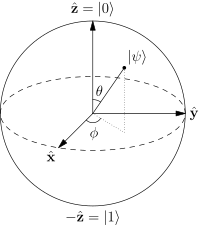
\includegraphics[width=0.3\columnwidth]{Bloch.png}
    \caption{Bloch sphere representation of a qubit}
    \label{fig:Bloch-Sphere}
\end{figure}
% The Bloch shpere also gives a nice intuition wher the \textit{pauli matrices}, $\sigma_x$, $\sigma_y$ or $\sigma_z$ on a state corresponds to rotating the qubit on one of the axis

\subsubsection{Wigner Function}
The \textit{Wigner Function} is yet another powerful visualization tool of a quantum system. The Wigner function is the \textit{distribution} of the \textit{phase space} of a quantum \textit{density operator}. In a classical view, thinking of the phase space as a distribution might seem weird at first, but for quantum system, where there is a fundamental uncertainty in the position and momentum, a phase space only makes sense as a distribution.

The Wigner function of a particle with wave function $\psi(x)$, is defined as 
\[
    W(q, p) := \frac{1}{\pi \hbar} \int_{-\infty}^\infty \psi^*(q + y) \psi(q - y) e^{\frac{2ipy}{\hbar}} dy
\]
An interesting example to use of the Wigner function is looking at the Wigner function of a Fock state. Since the Fock state represents a number of photons in a cavity, we can imagine how for each photon, by definition, is with constant $q^2 + p^2$, so it would create a circle around the center in the Wigner function. I won't prove the actual equation for the Wigner distribution of the number states, you can do so from the definition of the Wigner function. The expression is
\[
    W_n = \frac{2}{\pi}(-1)^n L_n[4(q^2 + p^2)]e^{-2(q^2 + p^2)}
\]
More importantly, we can look at a heat map of the Wigner function, this is a nice visual aid to see the state. here's an example with $\ket{4}$ state
\begin{figure}[H]
    \centering
    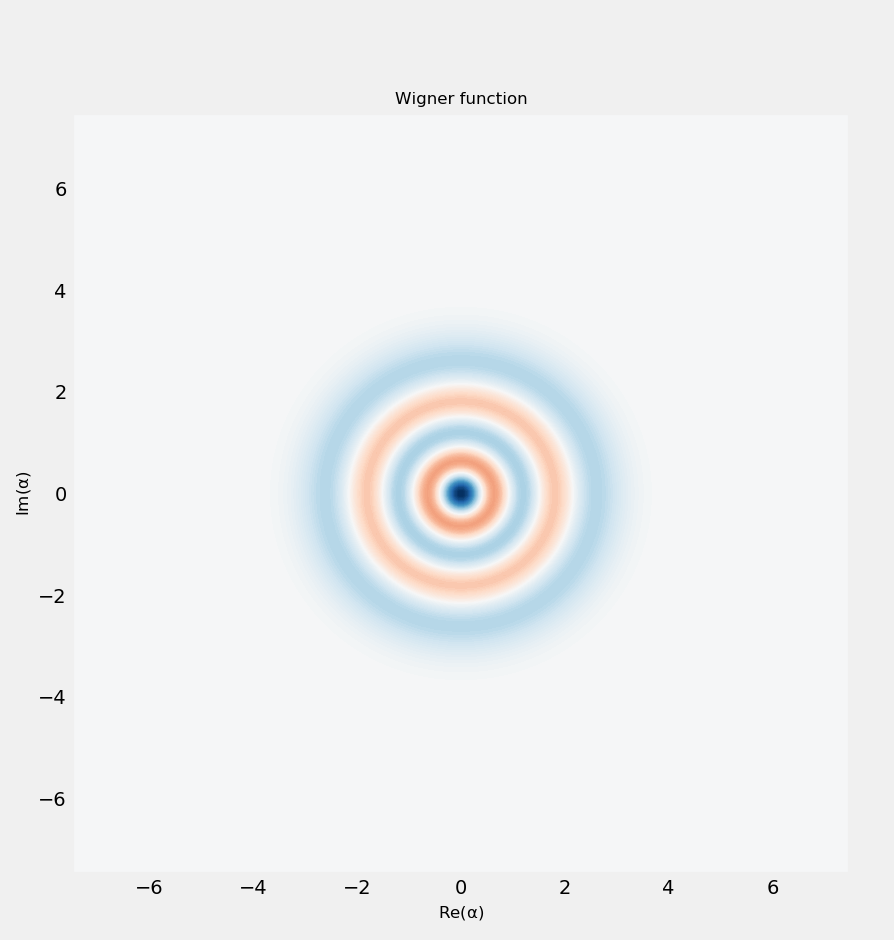
\includegraphics[width=0.4\columnwidth]{Wigner.png}
    \caption{Wigner distribution of the $\ket{4}$ Fock state}
    \label{fig:Fock-State-Wigner}
\end{figure}


% \newpage
% \section{Our System}

% \subsection{The cavity}

% \subsection{The Transmon}

% % \subsection{The Oscillator}

% \subsection{Describing the System Mathematically}  % TODO: Mention the JC model
% To describe the system mathematically we are going to calculate it's Hamiltonian, that way we can run simulations of the system with the Schrodinger equation.\par
% We can partition the system into different parts and analyse each part individually, so the total system Hamiltonian will be:

% \begin{equation}
% H(t) = H_{Oscillator} + H_{Transmon}+ H_{Interaction} + H_{Drive}(t)
% \end{equation}

% We'll begin by the easy to characterize, Transmon And Oscillator, they are a simple quantum system that can be described by the uppering and lowering operators \footnote{See appendix A}. We can write:
% \begin{equation}
% H_{Oscillator} = \omega_C a^\dag{}a
% \end{equation}
% \begin{equation}
% H_{Transmon} = \omega_T b^\dag{}b
% \end{equation}
% We can find $\omega_C$ and $\omega_T$ experimentally. % TODO: Maybe add a few words about how to do so and about the fact that this is only an harmonic approximation
% \par
% The next part to characterize is the interaction(See appendix A), by the Jaynes–Cummings model, we can write the interaction Hamiltonian as:
% \begin{equation}
% H_{Interaction} = \chi a^\dag{} a  b^\dag{} b % Again, this is only an harmonic approximation
% \end{equation}
% Again, we can measure $\chi$ experimentally.  % TODO: Maybe add more about how it's done
% \par
% Finally, we can characterize the driven and most important part of the system. It can be written as: % TODO: Add more about how do you get to that equation. Is it from Maxwell?
% \begin{equation}
% H_{Drive} = \epsilon_C(t)a + \epsilon_T(t)b + h.c.
% \end{equation}
% Or as(expanding the hermitian conjurgate):
% \begin{equation}
% H_{Drive} = \epsilon_{I_C}(t)(a + a^\dag{}) + \epsilon_{Q_C}(t)(a - a^\dag{})i + \epsilon_{I_T}(t)(b + b^\dag{})+ \epsilon_{Q_T}(t)(a - a^\dag{})i
% \end{equation}
% each \(\epsilon\) is a pulse that we will optimize with GRAPE as described in much details in the next chapter.
\subsection{References and Further Readings}
The standard introductory book on this subject(which is also the one I used for reference) is "\textbf{Introductory Quantum Optics}" by Christopher C. Gerry and Peter L. Knight.

Another great resource is the series of online lectures taught by Prof. Alain Aspect from École Polytechnique university.

\newpage
\section{Optimal Control}\label{chap:optimal}
This chapter is the main topic of this project, we tackle the problem of \textit{Quantum Optimal Control}. If we have a quantum system, the way we control the system is by sending some (classical)electromagnetic pulse to the system. Now an obvious question arises, what is this pulse? How does it look like? sin? cos? In what frequency? Some other wave? What does it do?

Turns out this is not that simple of a question. In the rest of the chapter we'll try to give an answer to this question using something called \textbf{\textit{GRAPE}}.

\subsection{What's GRAPE}
Although in some cases we can calculate the pulse analytically, most of the time this isn't an option, so we need to use numeric means to find the pulse. To find the desired pulse through numeric means, we can model our system on a normal(boring) computer and simulate what happens when you send a pulse, then, we can try to change the pulse(in a smart way) until we get the desired effect. So for example, let's say we want to find the wave pulse that corresponds to the NOT gate, we can start by guessing some random wave(constant zero, sin and so on), the random wave probably won't act as a NOT gate, then, we change the wave a little bit many times and on each iteration the pulse acts more and more as a NOT gate.
% TODO: Change the first propesed
So what's GRAPE than? GRAPE in an acronym for \textit{\textbf{GR}adient \textbf{A}scent \textbf{P}ulse \textbf{E}ngineering}. When we model a quantum system, in our case, a qubit, we can model everything about the system using the Hamiltonian of the system. There's the Hamiltonian that nature gives us, of how a qubit behaves and how it interacts with it's surrounding. And there's the Hamiltonian we control, using classical electromagnetic control pulse. We can send any possible pulse, to account for that fact, we treat the pulse amplitude over time as a step-wise constant function. The wave is just an array with many variables and we want to find the best values that give the result that we want. Then we set a cost function \footnote{discussed in details in the next section} that tells us how close to what we want are the values of the pulse we sent. This cost function is a many dimensional function(each step of the wave is a dimension of the cost function), and we can find its gradient. Using the cost function and it's gradient we can use some optimization algorithm(mainly, the L-BFGS-B method) to find the maximum of the cost function that gives us the optimal wave to send to the cavity.

\begin{figure}[H]
    \centering
    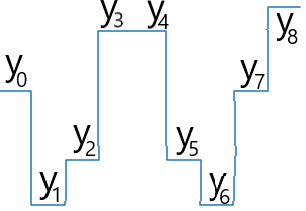
\includegraphics[width=0.3\columnwidth]{step-wise_example.png} % TODO: Change the image
    \caption{Example of a step-wise constant function as an array of numbers}
    \label{fig:step-wise-const}
\end{figure}

\subsection{The Cost Function}
So what is this cost function really? \textit{\textbf{Fidelity}}. It measures the "closeness" of two quantum states and varies between 0 and 1. So for example, the fidelity between state $\ket{0}$ and state $\ket{1}$ is equal to 0, because they are the most different two quantum states can be, while for example the fidelity between state $\ket{0}$ and state $\ket{0}$ is equal to 1, because they are the closest two states can be to each other(for a matter of fact, every state has fidelity 1 with itself and end fidelity 0 with an opposite state). But still, how do we calculate the fidelity between two states? well, turns out its very simple, it's just their product\footnote{Assuming both states are pure states and not density matrices}.

\begin{equation} \label{def:fid}
F(\psi_1, \psi_2) = \abs{\braket{\psi_1}{\psi_2}}^2
\end{equation}
We want to maximize the fidelity with GRAPE.

In a previous chapter we characterized the Hamiltonian of the system(equations (\ref{eq:JC-hamiltonian}) and (\ref{eq:dispersive-hamiltonian})), so now we can use the good old \textit{time-dependent Schr\"{o}dinger equation}:

\begin{equation}
i\hbar\frac{d}{dt}\ket{\Psi(t)} = \hat{H}\ket{\Psi(t)}
\end{equation}

The Hamiltonian of the system, as given in section 2.4, is of the  form % TODO: This will need to be chagnes(the section number to an actuall erference when chapter 2 is finished)

% TODO: Add explanation about that there are multiple different pulses and throughout the chapter we're referring to a single pulse which is most of the time not the case
\begin{equation} \label{eq:hamiltonianl_form}
H(t) = H_0 + \sum_k{\epsilon_k(t) H_k} % Maybe put the next part before the part about the Schrodinger equation
\end{equation}
where $H_0$ is the Hamiltonian of the system without the drives(given, for example, from the Jaynes-Cummings model or some other description of the system). Each $\epsilon_k(t)$ is the amplitude as a function of time of the control drive pulse, and each $H_k$ is the Hamiltonian describing the control pulse interaction with the system, we call these Hamiltonian the \textit{drive hamiltonians}. Our goal with GRAPE is to find optimal $\epsilon_k(t)$.

Because of the way this Hamiltonian is built, on each constant step of the pulse amplitude functions $\epsilon_k(t)$ function, the entire Hamiltonian is constant, and luckily for us, the solution of the Schrodinger equation for a constant Hamiltonian is pretty simple and given by
\begin{equation}
U(t) = e^{-\frac{i}{\hbar}\int_{T_0}^{T_1}H(t)dt}
\end{equation}
Because we chose $T_0$ and $T_1$ as the end points of a step of the functions, the total Hamiltonian of the system is constant so the integral is just a simple multiplication by $T_1-T_0$ which we'll write as $\delta t$. So the solution is
\begin{equation}
U(t) = e^{-\frac{i\cdot \delta t}{\hbar}H(t)}
\end{equation}

In order to calculate the solution over all the pulse we need to solve for the first step, find the solution by the end of the time-step, then use it as the initial condition for the next time step. If we do so, we get that after $N$ time steps, the solution over these time step is simply the product of the solutions until that time step
\begin{equation}\label{eq:U_def_prod}
U(\epsilon(t)) = \prod_{k = 1}^NU_k
\end{equation}
Now with $U(\epsilon)$ in our hands, we can calculate the evolution of the state over time
\begin{equation}
\ket{\Psi_{final}} = U(\epsilon)\ket{\Psi_{initial}}
\end{equation}
This way if we want to calculate the fidelity after applying the drives we can simply calculate the fidelity between the wanted state and the final state,
\begin{equation} \label{eq:fidelity_sim}
F(\Vec{\epsilon(t)}) = F(\Psi_{target}, \Psi_{final}) = \abs{\bra{\Psi_{target}}U_N\ket{\Psi_{initial}}}^2
\end{equation}

Now, theoretically we can use an algorithm to try different waves until we find a wave that does what we want(brute force for example), but this will take to much time and the computation won't finish in any reasonable amount of time. Because of this, we'll want to use a smart search algorithm(such as L-BFGS-B) but to do so we need the gradient of the cost function(the variables of the cost function are the values of the steps of the drive pulses).

\subsection{The Gradient}
As mentioned, if we want to optimize the cost function efficiently we'll need to calculate the gradient of the cost function and use an optimization algorithm. We can obviously use the finite difference method to calculate the gradient but this method is heavy on the computation and using it kind of defeats the purpose of the optimization algorithm to be more efficient. We'll take a smarter approach to calculating the gradient.

We can start with looking at the expression for the overlap of the final state and the target wanted state. This is very similar to the fidelity, if we take the absolute value of the overlap and square it we get the fidelity. We'll work with the overlap for now since it's nicer to work with because it does not have an absolute value in the calculation, we'll go from the overlap back to the fidelity in the end.
\begin{equation} \label{def:overlap}
c = \braket{\Psi_{target}}{\Psi_{final}} = \bra{\Psi_{target}}U\ket{\Psi_{initial}}
\end{equation}
We want to differentiate this expression by each control parameter. U is defined as:
\[ U = U_N U_{n-1}...U_2 U_1 \]
And when differentiating by a control parameter only one $U_k$ is affected, so we can write,
\[
\frac{\partial c}{\partial \epsilon_k} = \bra{\Psi_{target}}U_N U_{N-1} ... U_{k+1}\frac{\partial U}{\partial \epsilon_k} U_{k-1} ...U_2 U_1\ket{\Psi_{initial}} 
\]
We can write that for a constant Hamiltonian(from Schrodinger's equation)
\[
    U_k = e^{-\frac{i\cdot \delta t}{\hbar}H(t)}
\]
We can approximate the derivative $\frac{\partial U_k}{\partial \epsilon_k}$ in the limit of small $\delta t$ by writing
\begin{equation*}
    \frac{\partial U_k}{\partial \epsilon_k} \approx -\frac{i\cdot \delta t}{\hbar}\frac{\partial H}{\partial \epsilon_k} \cdot e^{-\frac{i\cdot \delta t}{\hbar}H(t)} = -\frac{i\cdot \delta t}{\hbar}\frac{\partial H}{\partial \epsilon_k} U_k
\end{equation*}

We can use this expression as the gradient values but it's still rather complex computationally($o(N^2)$ complexity).\par
We can use a bit different method to calculate the gradient to save on the computation by reducing the overhead.

Now the derivative of the cost function by an amplitude of the wave has become
\begin{equation} \label{eq:cost_init_deriv}
    \frac{dc}{d\epsilon_k} = -\frac{i\cdot \delta t}{\hbar} \bra{\Psi_{target}}U_N U_{N-1}... U_{k+1}\frac{dH}{d\epsilon_k} U_{k} ...U_2 U_1\ket{\Psi_{initial}} 
\end{equation}
Let's define 2 wave wave functions $\psi_{bwd}$ and $\psi_{fwd}$, they will be the multiplication component before and after the derivative of H, so:
\begin{equation} \label{eq:cost-function-b/fwd}
    \frac{\partial c}{\partial \epsilon_k} =  -\frac{i\cdot \delta t}{\hbar}\bra{\psi_{bwd}^{(k+1)}} \frac{\partial H}{\partial \epsilon_k} \ket{\psi_{fwd}^{(k)}}
\end{equation}
We can easily see from \ref{eq:cost_init_deriv} that 
\[   
\ket{\psi_{fwd}^{(k)}} = 
     \begin{cases}
       \ket{\psi_{init}} &\quad\ k=0\\
       U_k \ket{\psi_{fwd}^{(k-1)}} &\quad\ otherwise\\
     \end{cases}
\]
\[   
\ket{\psi_{bwd}^{(k)}} = 
     \begin{cases}
       \ket{\psi_{targ}} &\quad\ k=N+1\\
       U_k^{\dag{}} \ket{\psi_{bwd}^{(k+1)}} &\quad\ otherwise\\
     \end{cases}
\]
Now all we need is to do $2N$ calculations in the beginning($N$ for $bwd$ and $N$ for $fwd$) then calculating the actual gradient is trivial multiplication from equation \ref{eq:cost-function-b/fwd}. This improves the computation complexity in an order of magnitude($o(N^2)$ to $o(N)$) and the memory complexity by is still in the same order of magnitude($o(N)$ to $o(3N)$).

It's important to note that $c$ is not the fidelity, but the overlap. We can get the fidelity from $c$ like so \footnote{See initial definitions of $c$ and the fidelity(\ref{def:overlap} and \ref{def:fid} respectively)}
\[
F = |c|^2
\]
since $c$ might be complex this derivative is a bit less trivial than it might look like. We can write $c(\vec{\epsilon})$ as $a(\vec{\epsilon}) + b(\vec{\epsilon})i$, where $a, b \in R$ and we get that 
\[
\frac{\partial F}{\partial \epsilon_k} = \frac{\partial |c|^2}{\partial \epsilon_k} = \frac{\partial ||a+bi|^2}{\partial \epsilon_k} = \frac{\partial (a^2 + b^2)}{\partial \epsilon_k} = 2(a\frac{\partial a}{\partial \epsilon_k} + b\frac{\partial b}{\partial \epsilon_k})
\]
We can notice that\footnote{$(\frac{\partial c}{\partial \epsilon_k})^*$ is the complex conjugate of the derivative of c} $c(\frac{\partial c}{\partial \epsilon_k})^* = a\frac{\partial a}{\partial \epsilon_k} + b\frac{\partial b}{\partial \epsilon_k} + (ab - \frac{\partial a}{\partial \epsilon_k}\frac{\partial b}{\partial \epsilon_k})i$, more importantly we can see that the real part of that expression is exactly what we need, putting it all into one formula we get
\begin{equation} \label{eq:fidelity_gradient_final}
    \frac{\partial F}{\partial \epsilon_k} = 2\cdot \Re{c(\frac{\partial c}{\partial \epsilon_k})^*}
\end{equation}
Now all you need is to plug \ref{eq:cost-function-b/fwd} and \ref{def:overlap} into \ref{eq:fidelity_gradient_final} and you got your gradient :)

Let's do a little test now to see that everything is working well. The simplest pulse you can send is the pulse that takes the qubit from being in state $\ket{0}$ to state $\ket{1}$. We discussed this situation in appendix \ref{appen:annalytic} so we know how the solution should look like. Running our GRAPE code with some random initial pulse we get
\begin{figure}[H]
    \centering
    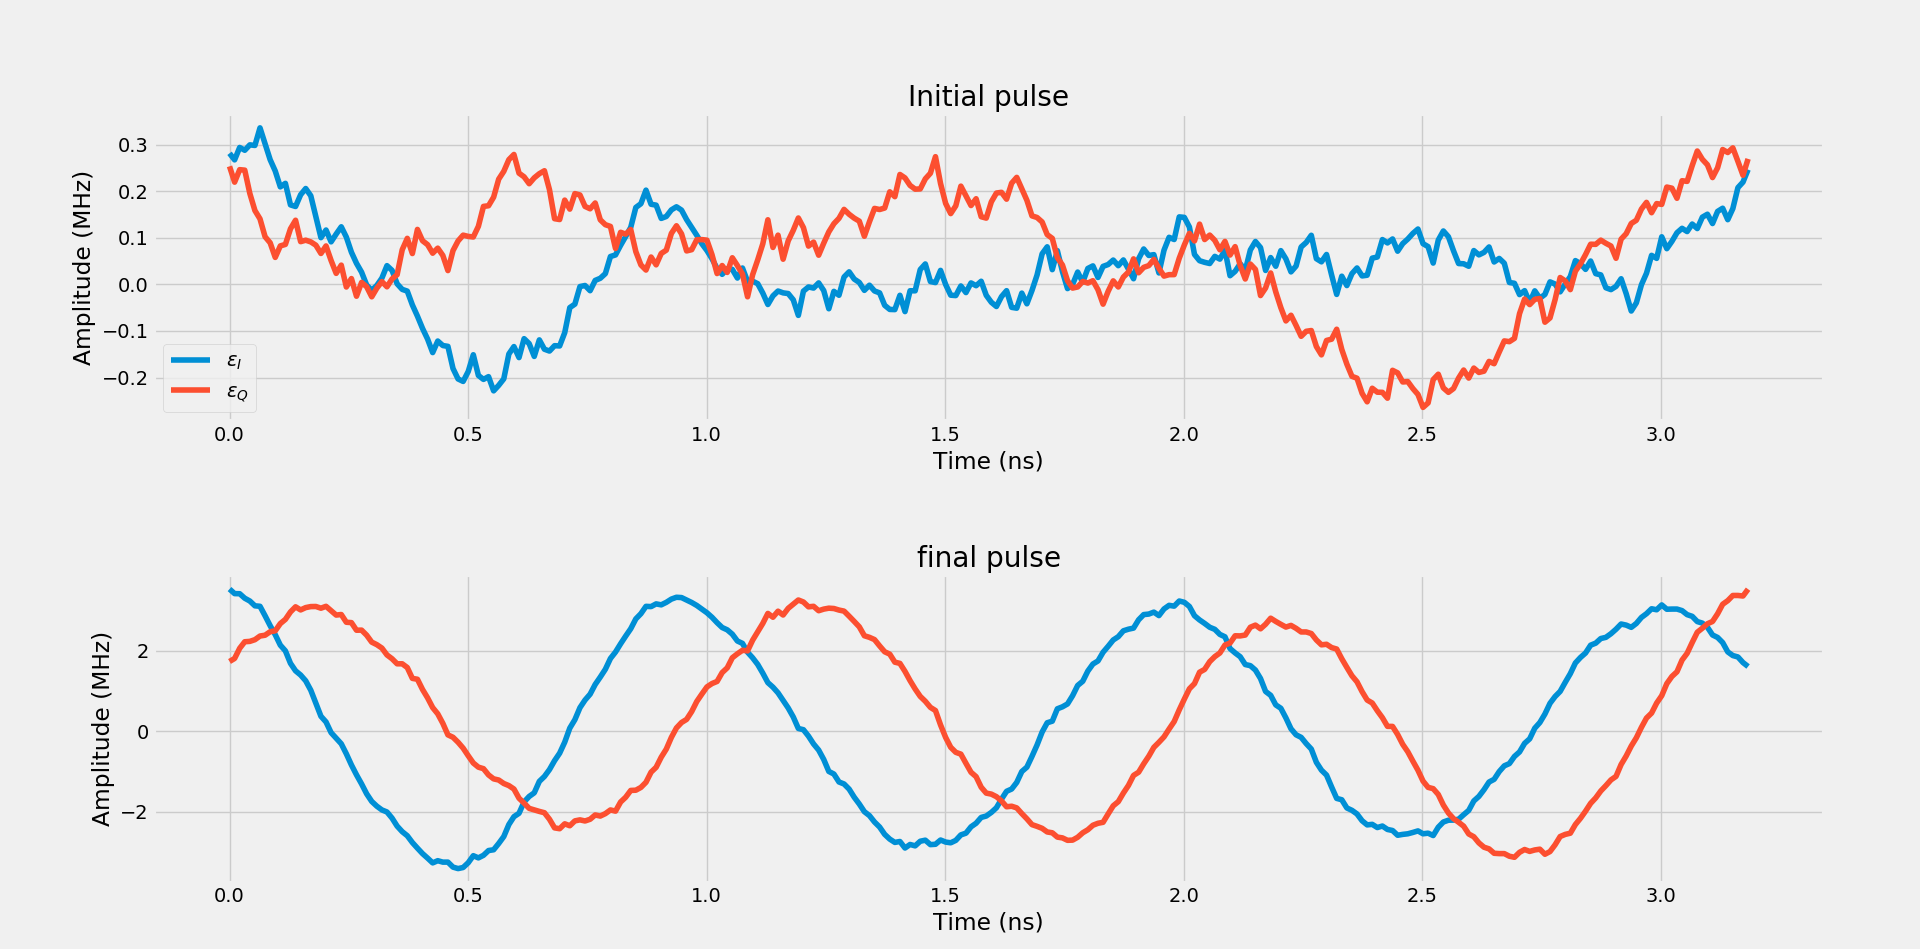
\includegraphics[width=1\columnwidth]{Results/No-Constraints-single-qubit/pulses-pretty2.png}
    \caption{First example of GRAPE from state $\ket{0}$ to state $\ket{1}$. This is almost perfect sin/cos waves as predicted analytically in appendix \ref{appen:annalytic}, but no exactly the same and not smooth for some reason}
    \label{fig:GRAPE-first-example}
\end{figure}
Amazing! From some random initial pulse we got sin and cos waves just as predicted in appendix \ref{appen:annalytic}.

Before we get too excited there are a couple of things weird with this pulse. The first, more obvious problem, is that although the waves are sin and cos as expected, they're still pretty jagged-y, there is some randomness on top of the wave and it's not as smooth as we expected. This is since small random changes don't really change the final result don't really change the final result\footnote{The positive noise cancels out the negative noise}. For reasons discussed in the next section we would like the pulse to be smooth.

Another problem that is not obvious right away we can see if we look at a graph of the level population over the duration of the pulse. We expect the graph to start at $1$ and end at $0$ for $\ket{0}$ and start at $0$ and end at $1$ for $\ket{1}$. Let's look at that graph for the initial random pulse and for the optimized pulse
\begin{figure}[H]
    \centering
    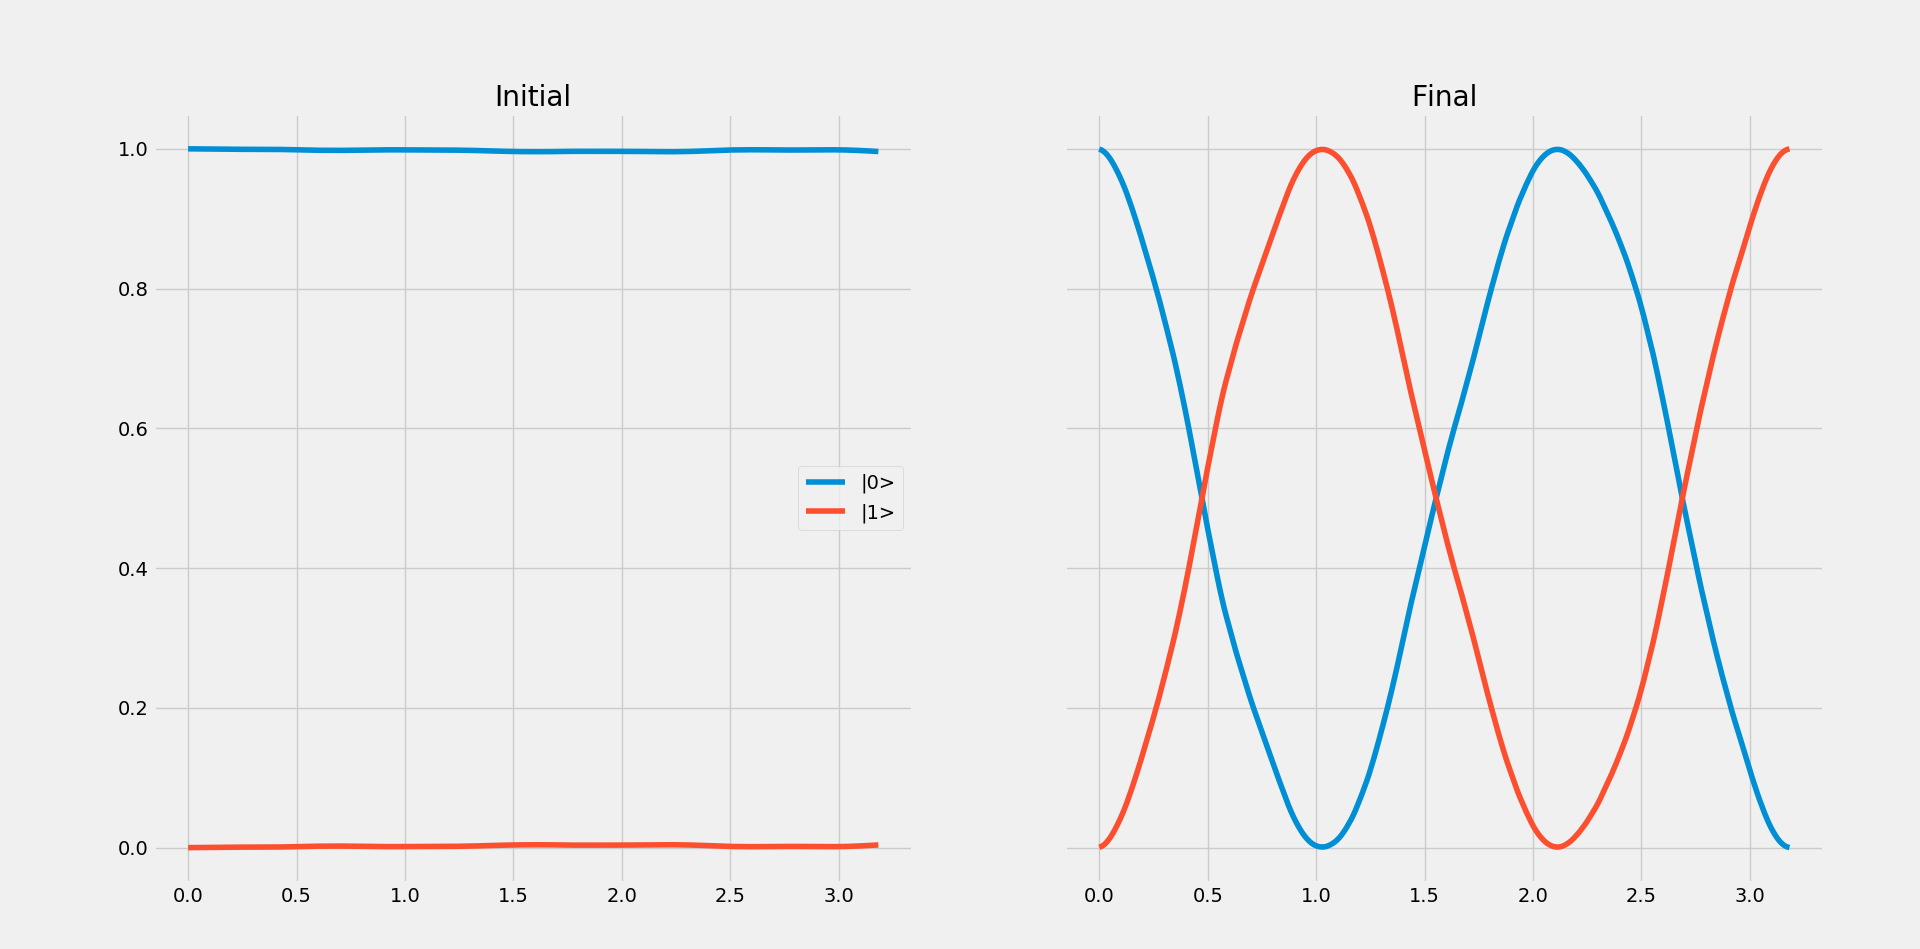
\includegraphics[width=1\columnwidth]{Results/No-Constraints-single-qubit/level-population-pretty2.png}
    \caption{Population of qubit levels over pulse duration. Before the optimization, the state of the qubit(population of ground and excited states) almost did not change at all. After the optimization, the qubit goes from state $\ket{0}$ to $\ket{1}$ to $\ket{0}$ to $\ket{1}$, doing some unnecessary back and forth between the states}
    \label{fig:GRAPE-first-example-level-population}
\end{figure}  % TODO: This graph is kinda false
As expected, the initial random pulse doesn't change the pulse almost at all. The optimized pulse on the other hand, WOW! What is this? It jumps between 0 and 1 too many times. Ideally, the population will change from 0 to 1(and vice-versa) smoothly only once.

This happens because the optimized pulse is wayyyy to strong, the amplitude of the pulse is huge! And well, as we defined the optimization, the algorithm doesn't care that the population does some weird stuff in the middle of the pulse as long as it ends at the desired state.

To solve these problems(and more that we'll talk about later) we introduce \textit{constraints} to the algorithm, as shown in great details in the next section.\footnote{I'll give a quick note just to be honest, since this is such a simple case, GRAPE works pretty well even without any constraints. I've carefully crafted conditions so that the final pulse wouldn't be smooth and so the level population would go crazy. This is what you'll see normally in more complex examples but I didn't want to go with a complex example since it would just complicate things without giving any real benefit}

\subsection{Constraints}
Having our simulation doing whatever it wants is nice and all but still unfortunately, we're living in the real world, and in the real world we can't just make ultra-fast frequencies at close to infinite power, it's just impossible because of the limitation of our devices. We need to add constraints to the cost function so we won't get solutions that use too much power or that change too rapidly.

We define a set of constraints on the solution ${g_i \ge 0}$(ideally $g_i=0$). We can associate a Lagrange multiplier $\lambda_i$ to each constraint. \newline
Now our goal is to maximize 
$$F(\vec{\epsilon}) - \sum_i \lambda_i g_i(\vec{\epsilon})$$
Let's add a constraint to each of the most problematic physical limitation
\subsubsection{Limiting the Pulse Amplitude}
This is the most obvious physical limitation, we can't generate pulses with infinite energy, so we have to restrict it. There are two ways we can do so, the first is to create a hard cut-of amplitude, no matter what, the amplitude will never go above this amplitude, this will usually be the limit of our pulse generator. But normally we don't want our generator to work at it's absolute limit\footnote{Not only that it might damage the device but also with stronger pulses the non-linear optics effects increase and then it's no fun :(}, so we can add also a soft amplitude maximum by "rewarding" the cost function to stay at a lower amplitude. Let's see how we would implement such a thing, starting with the hard cut-off.

Instead of controlling and changing the amplitude($\vec{\epsilon}$) directly, we'll introduce a variable $\vec{x}$ and relate them as
$$\vec{\epsilon} = \epsilon_{max}\tanh{\vec{x}}$$
As you properly guessed, $\epsilon_{max}$ is the maximum amplitude of the pulse.
Since the optimization algorithm can only change $\vec{x}$, the amplitude of the pulse will always be between $-\epsilon_{max}$ and $\epsilon_{max}$. Unluckily for us, this changes the gradient of the cost function since we now want the derivative with respect to $\vec{x}$ instead of $\vec{\epsilon}$. We can relate the two
\[
\frac{\partial F}{\partial \vec{x}} = \frac{\partial F}{\partial \vec{\epsilon}}\frac{\partial \vec{\epsilon}}{\partial \vec{x}} = \frac{\epsilon_{max}}{\cosh^2{\vec{x}}} \ \frac{\partial F}{\partial \vec{\epsilon}}
\]
We can use the derivative $\frac{\partial F}{\partial \vec{\epsilon}}$ we got from \ref{eq:fidelity_gradient_final} and simply calculate $\frac{\epsilon_{max}}{\cosh^2{\vec{x}}}$ and we again have the gradient.

For the soft limitation, there are two limitation we can make, linear and non-linear. The linear goal is for general preference of low amplitude pulses and the non-linear is if you have a specific \(\epsilon_{max,soft}\) that you want to be well below of(You can use both or either one depends on your desired pulse properties). We'll start with the linear case since it's simpler.

For the linear amplitude penalty all we want is that \textit{bigger amplitudes} \(\Rightarrow\) \textit{bigger cost function}, since our algorithm seeks to minimize the cost function, this will lead to the overall amplitude being smaller. The way we do so is simple, we can define a constraint \(g_{amp,lin}\) that sums all the amplitudes of the steps of the pulse, so
\[
    g_{amp,lin} = \sum_k |\epsilon_k|^2
\]
and we maximize the cost function as explained at the beginning of the section.

Still, since it is added to our cost function we need to find the gradient of the penalty as well. In the case it's rather simple since it's a basic parabola
\[
    \frac{\partial g_{amp,lin}}{\partial \epsilon_k} = 2\epsilon_k
\]
and now we have all we need in order to add this penalty to our cost function. Let's move on to the non-liner penalty.

% For the non-linear amplitude penalty we have a slightly different goal in mind
% TODO: Add here the non linear amplitude penalty


\subsubsection{Limiting the Pulse Bandwidth and Slope}
Again we encounter a physical limitation, we can't produce any pulse we want, there's a limitation of the maximum frequency our AWG(Arbitrary Waveform Generator) can create because the device can't change the voltage instantaneously. Again, like we had with the amplitude limit, there are 2 types of limits we can make, hard and soft. Let's start with the hard limit.

We have some frequency \( \omega_{max} \) which is the maximum frequency that our AWG can generate. To make sure that our simulation doesn't produce such a pulse we can go from time space to the frequency space with a Fourier transform(Discrete Fourier Transform to be exact).
\[
    \vec{\epsilon} = (DFT)^{-1} \vec{x}
\]
The numerical optimization algorithm controls \(\vec{x}\) which is in the frequency space. Now if we want to limit the frequency we can simply set to 0 any frequency that is above our maximum frequency.\footnote{Might be more efficient to set these frequency to 0 and not let the optimization algorithm to try to change them(living the completely out of the pulse then putting them back in as 0 after the optimization is finished)}
\[
    x(\omega > \omega_{max}) = 0
\]
The gradient of the new cost function is simply the Fourier transform of x
\[
    \frac{\partial \vec{x}}{\partial \epsilon_k} = (DFT) \frac{\partial \vec{\epsilon}}{\partial \epsilon_k}
\]
And we know \(\frac{\partial \vec{\epsilon}}{\partial \epsilon_k}\) from previous sections.
It's important to note that the hard cut-off of the amplitude and the hard cut-off of the frequency do not work together since one is in the time space and one is in the frequency space. This is not much of a problem since we can compensate with the soft limits that do work well together(mainly since they require adding to the cost function instead of changing coordinate). In my simulations I use the amplitude hard limit instead of the frequency one since it only requires "squishing" the function instead of going from time space to frequency space.

For the soft limits, we're limiting the slope(derivative) of the pulses and not the frequency directly. There are, again, two types of limits we can make, a linear limit and a non-linear limit. The linear limit simply incentives for a lower maximum slope overall, and the non-linear limit incentives a specific maximum soft limit on the slope, we can use the two together. Let's start with the simpler, linear limit.

The slope of a step function is simply \(\epsilon_{k+1} - \epsilon_{k}\), we want to limit the size of the slope so we'll look at the expression \(|\epsilon_{k+1} - \epsilon_{k}|^2\) instead. Summing all the slopes(to get an overall slope size of the entire pulse) we get the expression\footnote{Note that we have a problem at the edges since the slope of the end points is not well defined, we'll fix this problem later but for now we just ignore the last point \(k=N\)}
\begin{equation}\label{eq:g_slope,lin}
    g_{slope, lin} = \sum_{k=0}^{N-1} |\epsilon_{k+1} - \epsilon_{k}|^2
\end{equation}{}
Remember that for each limit we associate a number \(\lambda_{slope, lin}\) that is the "strength" of the limit, and that the cost function now becomes: \textit{*old cost function*} + \(\lambda_{slope, lin} g_{slope, lin}\), so we need to calculate the gradient of this limit and add it to the total gradient of cost function.

Unlike the amplitude, since the slope of the boundaries is not well defined we'll have the edges defined differently then the center of the pulse. The gradient of \(g\) in the center is a simple derivative, notice that each \(\epsilon_k\) appears only twice in the sum
\[
    \frac{\partial g_{slope, lin}}{\partial \epsilon_k} = 4\epsilon_k - 2(\epsilon{k+1} + \epsilon{k-1})
\]
It's nice to see that the expression looks like how'd you numerically estimate the second derivative, since the gradient of the slope(which is the derivative) is the second derivative, this is nice and reassuring :). Now we need to define the gradient at the edges, you can see that the derivative of \(\epsilon_k\) depends on his 
+neighbors on both sides, since the first and last element of the pulse don't have 2 neighbors they are treated a little differently. each of the edges appears only once in the sum \ref{eq:g_slope,lin} unlike the others that appear twice, we can simply take the derivative of that one term and get
\begin{align*}
    &\frac{\partial g_{slope, lin}}{\partial \epsilon_0} = 2(\epsilon_1 - \epsilon_0) \\
    &\frac{\partial g_{slope, lin}}{\partial \epsilon_N} = 2(\epsilon_N - \epsilon_{N-1})
\end{align*} % TODO: This definitely needs some changing!!!
And now the slope soft linear limit is defined and so is it's gradient.

Now, before we continue to the non linear limit, we'll add another small constraint that will also solve the problem of the slope at the boundaries(you can think of it as a sort of boundary condition). It might seem weird at first, but we want to pulse to zero-out at the edges(the amplitude of the first and last steps of the pulse being equal to 0), this is since our AWG device can't immediately start a pulse with some amplitude, it can't get from 0 to that amplitude instantaneously(for the same reason we limit the slope in the first place). This could be achieved by simply setting the first and last steps of the pulse and their gradient to 0.
\[
    \epsilon_0 = \epsilon_N = \frac{\partial \ Cost}{\partial \epsilon_0} = \frac{\partial \ Cost}{\partial \epsilon_N} = 0
\]
This solves the problem we were trying to solve we were having with the slope at the boundaries, since the gradient is 0 at the edges and does not depend on it's neighbors. We can move on to the non-linear limitation now.

% As we mentioned earlier, the goal of the non-linear limitation is when we have a specific bandwidth to be well below off, the could be achieved thanks to the fact that exponents grow really fast
% \[
%     Add\ equation\ here
% \]
% TODO: Add here but more importantly change how is the goal of the non-linear limitation explained.

Now that we have both amplitude constraint and bandwidth constraint we can use them to get a nice, smooth solution, that any wave generator would be happy to produce
\begin{figure}[H]
    \centering
    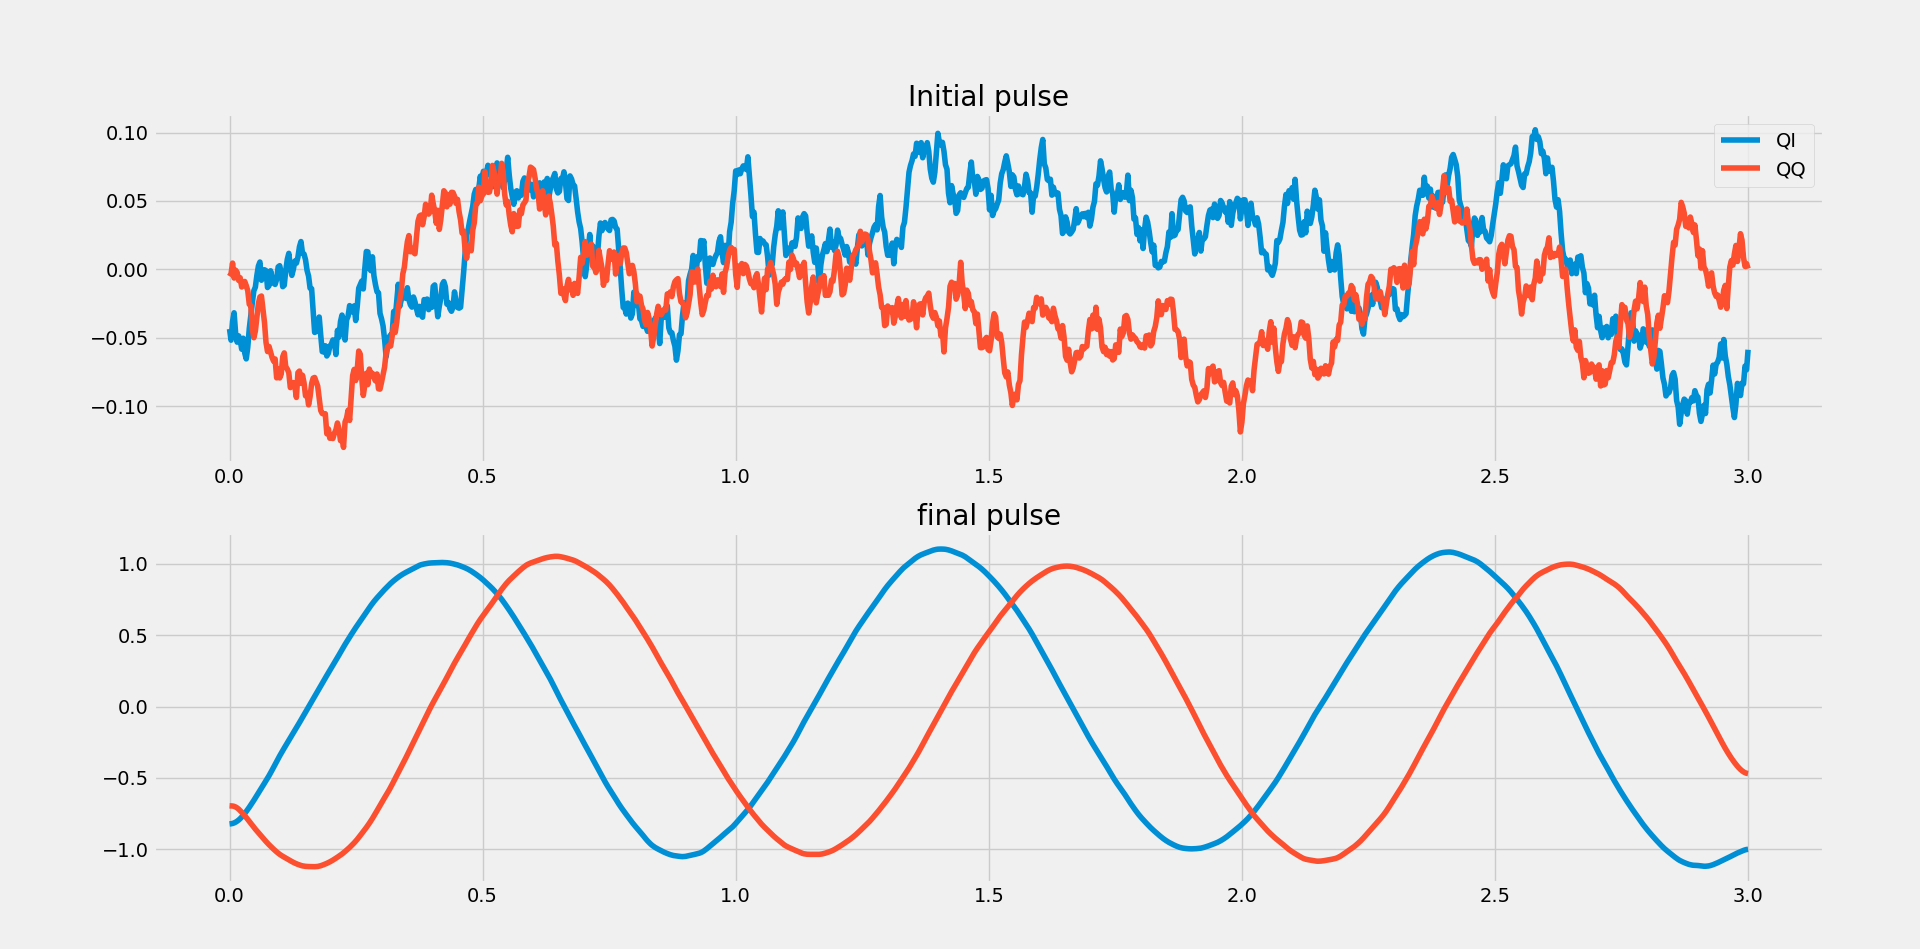
\includegraphics[width=1\columnwidth]{Results/qubit-band-amp-const/pulses.png}
    \caption{Control pulses before and after GRAPE optimization with amplitude and bandwidth constraints}
    \label{fig:band-amp-const-qubit}
\end{figure}
This looks nice and what we expected it to look like.

The more important thing is that if we look at the population of the levels over time, it does exactly what we want, go from state $\ket{0}$ to state $\ket{1}$ without going back and forth
\begin{figure}[H]
    \centering
    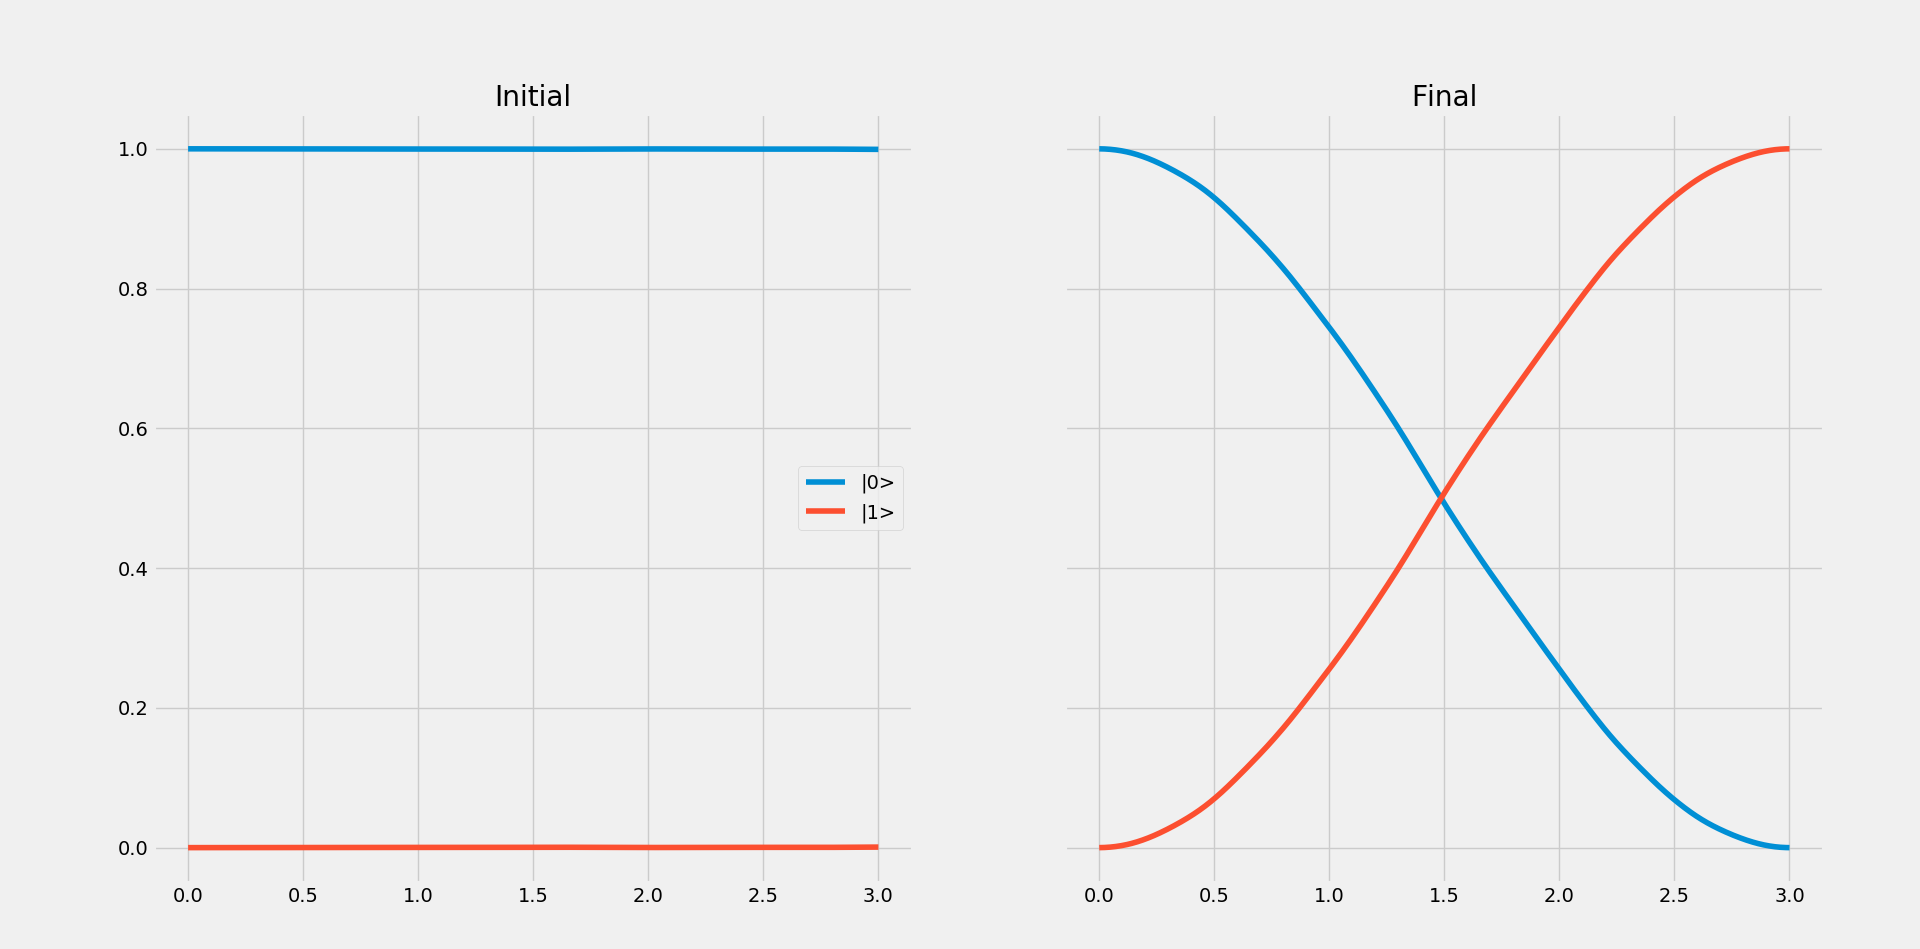
\includegraphics[width=1\columnwidth]{Results/qubit-band-amp-const/level-population.png}
    \caption{Population of qubit levels over pulse duration. Before the optimization, the state of the qubit(population of ground and excited states) almost did not change at all. After the optimization, the qubit goes from state $\ket{0}$ to $\ket{1}$}
    \label{fig:band-amp-const-level-population}
\end{figure}

Another interesting metric of the success of this pulse is the path of the qubit on the Bloch sphere over time(see the last section in chapter \ref{chap:quantum-optics}). Plotting the populations on the Bloch sphere we get 
\begin{figure}[H]
    \centering % TODO: Replace with actuall bloch sphere
    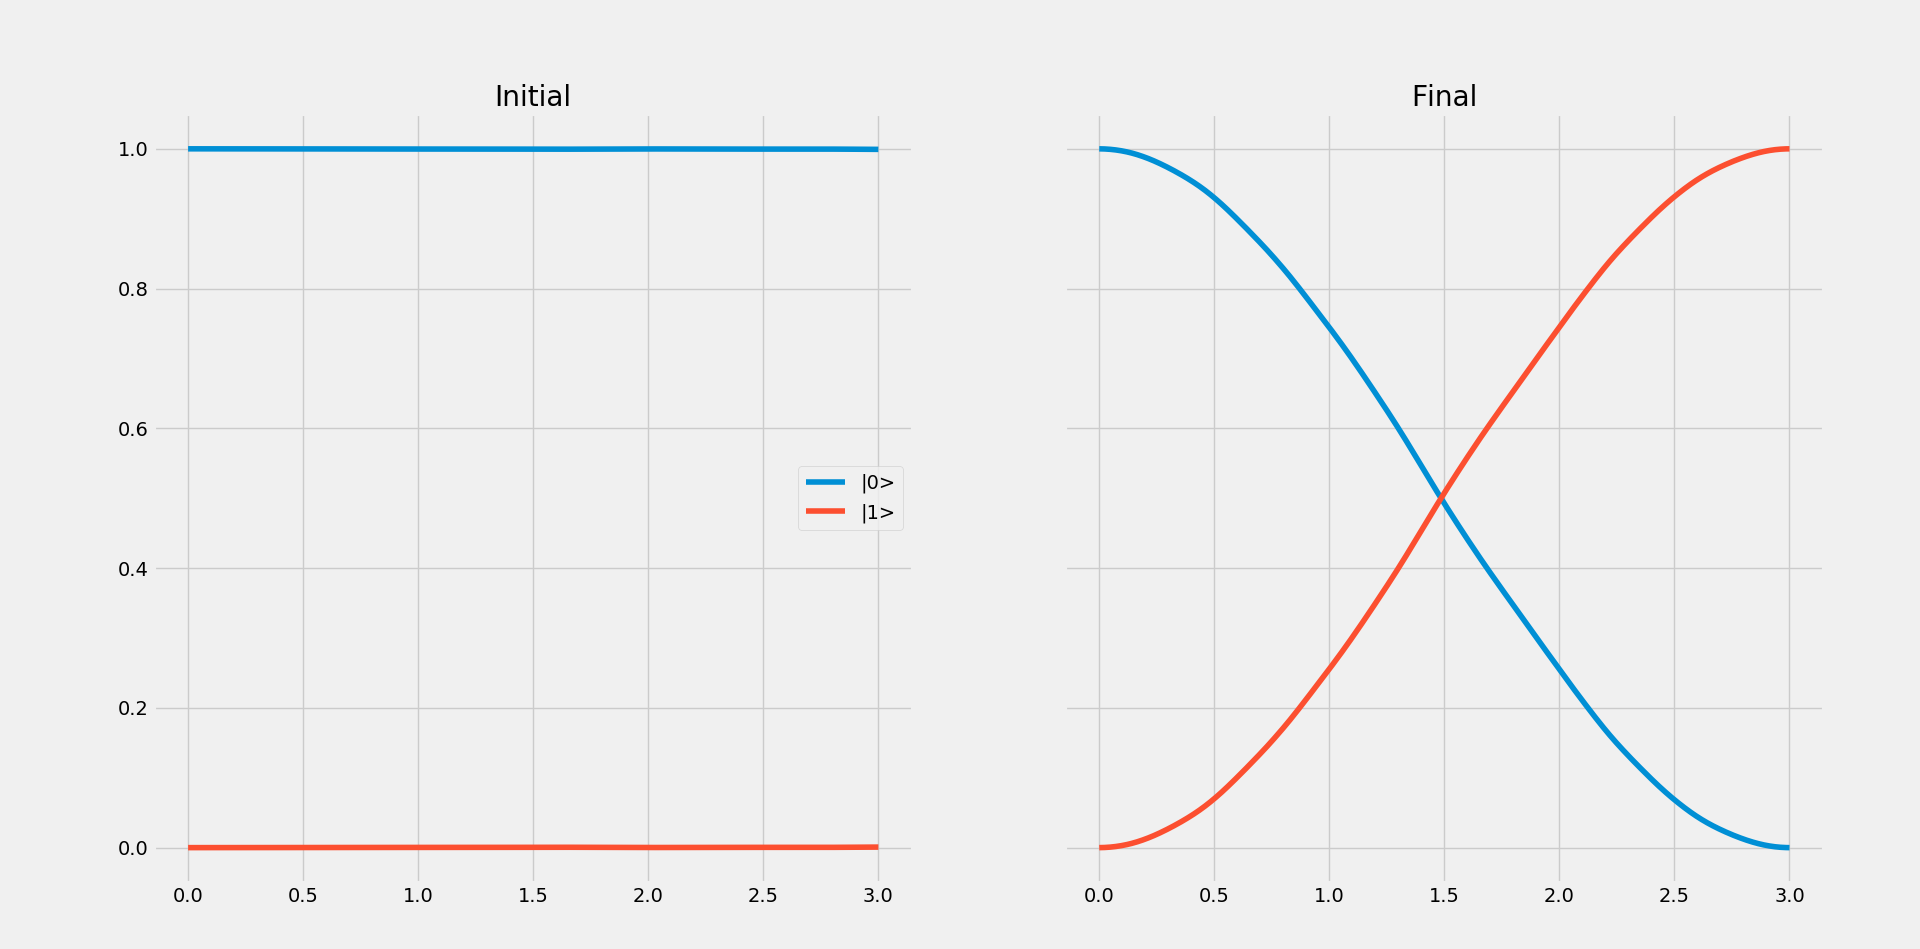
\includegraphics[width=1\columnwidth]{Results/qubit-band-amp-const/level-population.png}
    \caption{Path of the qubit along the Bloch sphere. The qubit goes from state $\ket{0}$ to state $\ket{1}$, preforming one loop on the sphere, the arrows represent the initial state and the target state, and the points represent the path of the state of the qubit}
    \label{fig:band-amp-const-blcoh}
\end{figure}
As you can see, the path of the qubit isn't a straight line, but some loop, completing a full rotation around the $\hat{z}$ axis. This is explained by the fact that the base Hamiltonian of the qubit is $\omega \hat{\sigma}_z$, where $\hat{\sigma}_z$ is the third Pauli matrix, this matrix corresponds to rotation of the Bloch sphere around the $\hat{z}$ axis(it's common to define $\hat{Z} = \hat{\sigma}_z$ because of this property). This is why we can think of the entire Bloch sphere as always rotating with frequency $\omega_0$ around the $\hat{z}$ axis, this is why a "straight" path is actually one that does one loop around the $\hat{z}$ axis.
% \subsection{Adding the Cavity}
% \subsubsection{From Pure State to Density Matrix}
% When we want to describe a qubit-cavity system we need to go from pure states to density matrices(explained in more details in a moment). Unluckily for us, this means changing how we calculate the fidelity and it's gradients, so we'll need to change some of the equations we used in the previous section to get GRAPE to work in such a system.
% TODO: Need to add here alot, maybe change the wording
\subsubsection{Limiting Pulse Duration}
As much as I wouldn't mind waiting a few nanoseconds longer for the qubit operation to end, the qubit itself isn't as patient as me. A state-of-the-art qubit would last, at most, one second(and that's a very conservative estimation), we simply don't have the time to wait for the operation to end if we want to run some complicated quantum circuit. This is why we want to add a constraint on the duration of the pulse, that way, if we give the pulse 5ns to finish, and a solution of 3ns exists, the optimization algorithm would(hopefully) find the 3ns solution and the rest of the time until the end of the duration will do nothing.
% TODO: Add figure of such pulse

The constraint is fairly straight forward, add a penalty for any time a fidelity of 1 isn't achieved. Put into an equation we get
\[
    g_{duration} = \sum_{i = 0}^{N-1} (1 - F_i)
\]
Where $F_i$ is the fidelity at time step $i$.

We can rather simply calculate the fidelity at any given time since the current way we calculate the fidelity, the state of the qubit at each time step is calculated(although not used, only calculated for the sole purpose of calculating the state at the next time step), we can simply modify the loop that calculates the final state into giving the fidelity at each time step and sum the results. 
% TODO: Maybe remove some of the technical details about the code and the implementation

Luckily for us, the calculation of the gradient is also pretty simple, the gradient of the fidelity at each time step is calculated the same as the gradient of the fidelity we calculated in the beginning of the chapter\footnote{note that $\epsilon_k$ only appears in the expression for $F_i$, if $i > k$, so the sum starts at $i = k$}
\[
    \frac{\partial g_{duration}}{\partial \epsilon_k} = -\sum_{i = k}^{N-1}\frac{\partial F_i}{\partial \epsilon_k}
\]
% TODO: I think I can find a more efficient solution
% TODO: Got to check this in the code and ask serge for his opinion
The calculation of the gradient % TODO: Need to continue thhis line. Don;t rememeber what I originally wanted

The pulse duration constraint works nicely to complete the other constraints. Without this constraint, the pulse will "try" to use all it's time to get the result we desire, and when running the algorithm without the constraint we can get problems if the duration we gave to the pulse is too long or too short. With this constraint on, we can simply give the algorithm a duration that we know for sure is more then the minimum required time and the algorithm will simply use the minimum time it need and no more. On the other hand, if we didn't have the amplitude(and bandwidth) constraints, the algorithm might find that it's best to just give a huge pulse for a tiny amount of time, but that's not physically possible as we discussed. This is why we can think of the constraints working together to "box in" the pulse into an ideal size.

If we run GRAPE now, with all the constraints together, and look at the population of all the level over the duration of the pulse, we get
\begin{figure}[H]
    \centering
    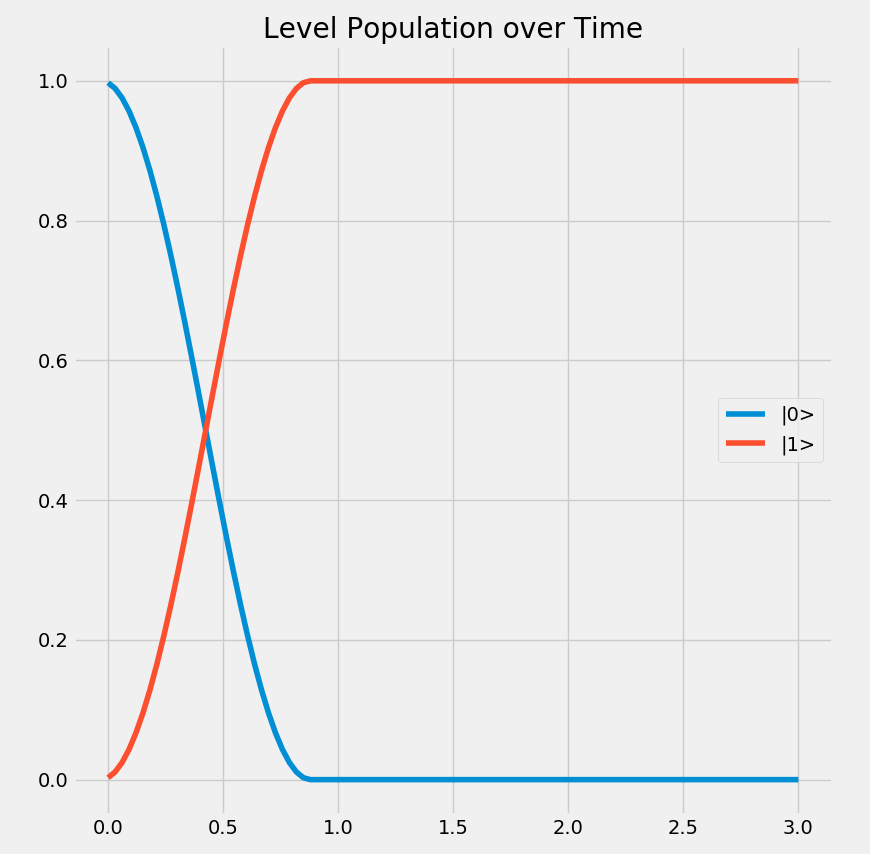
\includegraphics[width=0.5\columnwidth]{Results/duration-constraint/level-population.png}
    \caption{Level population of each state as a function of time over the duration of the pulse.}
    \label{fig:dur-penelty}
\end{figure}

As expected, we get exactly what we want, the pulse uses the least amount of time that it needs and then stop. This way, if we pick a long duration for the pulse, instead of the pulse trying to fill the entire time at a very low amplitude, or do several of loops before arriving at the target, the qubit simply takes exactly the amount of time that it needs to get to the desired state under all of the constraints and then stops.

\subsection{Implementing Qubit Operations with GRAPE}

\subsubsection{DRAG - Imperfect Qubits} \label{sec:DRAG}
When we did all of our calculation on the qubit we didn't include one detail, it's really hard to create a qubit, there's a reason why I don't have my quantum laptop yet after all :(. In the way our qubits are implemented, there are actually more then 2 levels. It's not a 2 level system but we treat it as one since the higher levels are off-resonance\footnote{as explained in the beginning}, but still there's a chance some of the higher levels will get excited by our pulses or some other physical phenomena and we want to account for it. The way we can do so is with the Derivative Removal via Adiabatic Gate(DRAG) algorithm. The idea being we make the qubit in the simulation to be more then a 2 level system, change the Hamiltonian a little bit(as you'll see later) so it accounts for the off-resonance higher levels and use the same grape algorithm to optimize for the entire system and not only the lower 2 levels.

Before we continue to implement DRAG, let's see if the 3rd level really is that of a problem, we'll run a simulation of GRAPE just as we did before but this time with 3 levels instead of 2, and the 3rd level should start and end at 0 population. We get after running GRAPE
\begin{figure}[H]
    \centering
    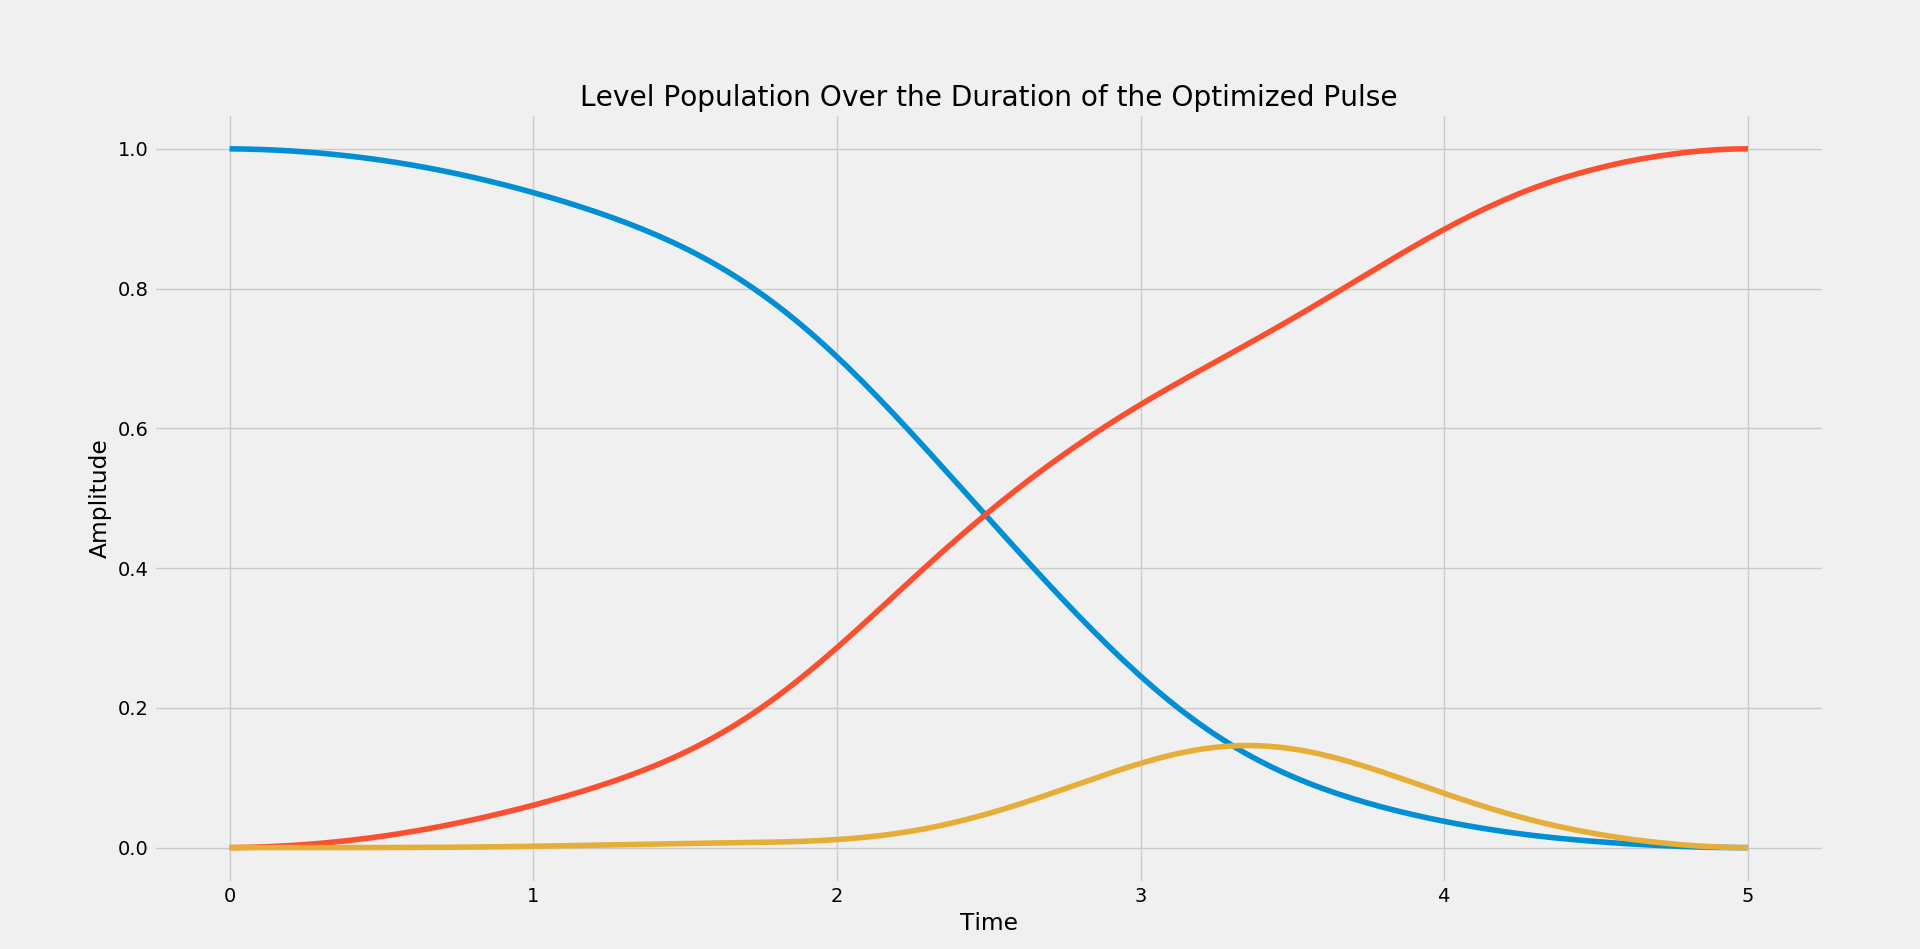
\includegraphics[width=1\columnwidth]{Results/Before-Drag/level-population-pretty.png}
    \caption{Level population of the 3-level qubit over the duration of the pulse calculated by the GRAPE algorithm we have so far}
    \label{fig:before-DRAG} % TODO: Replace these graphs with the actuall graphs
\end{figure}
Well yes, the forbidden layer did start and end at $0$ population, but in the middle the qubit really became a 3 level system with the population of the forbidden level being really dominant around time $3.5$! This isn't one of the first two levels, we want to treat the system as if there are only two levels and the forbidden level should be negligible. More then that, the solution is noisy and not as smooth as we want, that is since it does the state transfer in a really unconventional manner, if we gave the algorithm a penalty on the forbidden level we would get a more conventional solution(sinusoidal).

We can't simply replace the qubit with a 3 level system and make the target of the third level always 0 and call it a day. We can't treat higher levels as another qubit level, they are unwanted and we need to give them a penalty so the probability of being in a higher level would be always almost zero and change only a tiny bit. There are many ways we could implement such a penalty, the most obvious way is by simply making the probability to be in an higher level into a penalty, summing over all time we get(We'll call the third level of the qubit \(\ket{f}\) to not be confused with the \(\ket{3}\) Fock state(photon number state))\footnote{If we wanted to accounted for higher levels we can sum over the sum for each level}  % TODO: I need to reword a lot and explain where the hell did the equation come from
\[
    g_{forbidden} = \sum_{i=0}^{N - 1} \abs{\braket{f}{\psi_{fwd}^{(i)}}}^2 
\]
We already have \(\psi_{fwd}^{(i)}\) that we calculated earlier, so for so good.

Now moving to to complex part of DRAG, the gradient. Let's again define the overlap
\[
    c_{f} = \sum_{i=0}^{N - 1} \braket{f}{\psi_{fwd}^{(i)}}
\]
now to calculate the gradient we'll derive over \(\epsilon_k\)
\[
    \frac{\partial c_{f}}{\partial \epsilon_k} = \frac{\partial}{\partial \epsilon_k}\sum_{i=0}^{N - 1}  \braket{f}{\psi_{fwd}^{(i)}} = \sum_{i=0}^{N - 1} \frac{\partial}{\partial \epsilon_k} \braket{f}{\psi_{fwd}^{(i)}}
\]
recall that \(\psi_{fwd}^{(i)} = U_i \cdot U_{i-1} \cdot ... \cdot U_1 \ket{\psi_{initial}}\), \(U_k\) only appears for \(i > k\), so we can start the sum from $i = k$. We'll also expand $\psi_{fwd}^{(i)}$ into what it is and get
\[
    \frac{\partial c_{f}}{\partial \epsilon_k} = \sum_{i=k}^{N - 1} \frac{\partial}{\partial \epsilon_k} \bra{f}U_i \cdot ... \cdot U_0 \ket{\psi_{initial}}
\]
the only element that's dependent on $\epsilon_k$ is $U_k$, so we can rearrange the equation as
\begin{align*}
    \frac{\partial c_{f}}{\partial \epsilon_k} &= \sum_{i=k}^{N - 1} \bra{f}U_i \cdot ...\cdot \frac{\partial U_k}{\partial \epsilon_k} \cdot ... \cdot U_0 \ket{\psi_{initial}} \\
    &= \sum_{i=k}^{N - 1} \bra{f}U_i \cdot ...\cdot i \cdot \delta t\frac{\partial H_k}{\partial \epsilon_k} U_k\cdot ... \cdot U_0 \ket{\psi_{initial}} \\
    &= i \cdot \delta t \sum_{i=k}^{N - 1} \bra{f}U_i \cdot ... \cdot U_{k+1} \cdot \frac{\partial H_k}{\partial \epsilon_k}\ket{\psi_{fwd}^{(k)}}
\end{align*}
Now just to keep everything simple and maintainable, we'll define
\[
    \bra{\phi_{bwd}^{(i,k)}} = \bra{f} U_i \cdot ... \cdot U_{k+1}
\]
The equation for the overlap now becomes
\[
    \boxed{\frac{\partial c_{f}}{\partial \epsilon_k} = i \cdot \delta t \sum_{i=k}^{N - 1} \bra{\phi_{bwd}^{(i,k)}} \frac{\partial H_k}{\partial \epsilon_k} \ket{\psi_{fwd}^{(k)}}}
\]
Now we got all we need to calculate the penalty of the occupying the higher level and it's gradient. This isn't a perfect solution though, for $N$ time steps we need to do $o(N^2)$ calculations to get $\bra{\phi_{bwd}^{(i,k)}}$, this slows down the calculation considerably\footnote{it makes to calculation run around 100 times slower, pretty bad considering it's just a penalty} and there is a lot of overhead in the way we calculated $\bra{\phi_{bwd}^{(i,k)}}$. We can use a smarter way to calculate it.

Consider a function, very similar to  $\bra{\psi_{bwd}}$ we had earlier(in fact, it's the same function minus multiplying by the target state on the left)
\[
    \psi_{bwd}^{(k)} = U_NU_{N-1}...U_{k+2}U_{k+1}
\]
taking the inverse of the resulting matrix we get
\[
    (\psi_{bwd}^{(i)})^{-1} = U_{i+1}^{-1}U_{i+2}^{-1}...U_{N-1}^{-1}U_{N}^{-1}
\]
by multiplying the two matrices we get(defining their product as $\phi_{bwd}$)
\[
    \phi_{bwd}^{(i,k)} = (\psi_{bwd}^{(i)})^{-1}(\psi_{bwd}^{(k)}) = (U_{i+1}^{-1}\cdot...\cdot U_{N}^{-1})(U_N\cdot...\cdot U_{k+1}) = U_{i}\cdot...\cdot U_{k+1}
\]
This is exactly what we wanted! from this we'll define
\[
    \bra{\phi_{bwd}^{(i,k)}} = \bra{f}\phi_{bwd}^{(i,k)}
\]
remember that $\psi_{bwd}$ was already calculated from the gradient calculation, taking the inverse of $\psi_{bwd}$ isn't affected by how many time steps there are, also the multiplications between $\psi_{bwd}$, $(\psi_{bwd})^{-1}$ and $\bra{f}$ isn't dependent on the amount of time steps, so the entire calculation is $o(1)$ complexity. We went from $o(N^2)$ to $o(1)$ with this simple trick!

Let's run now the algorithm and get some results
\begin{figure}[H]
    \centering
    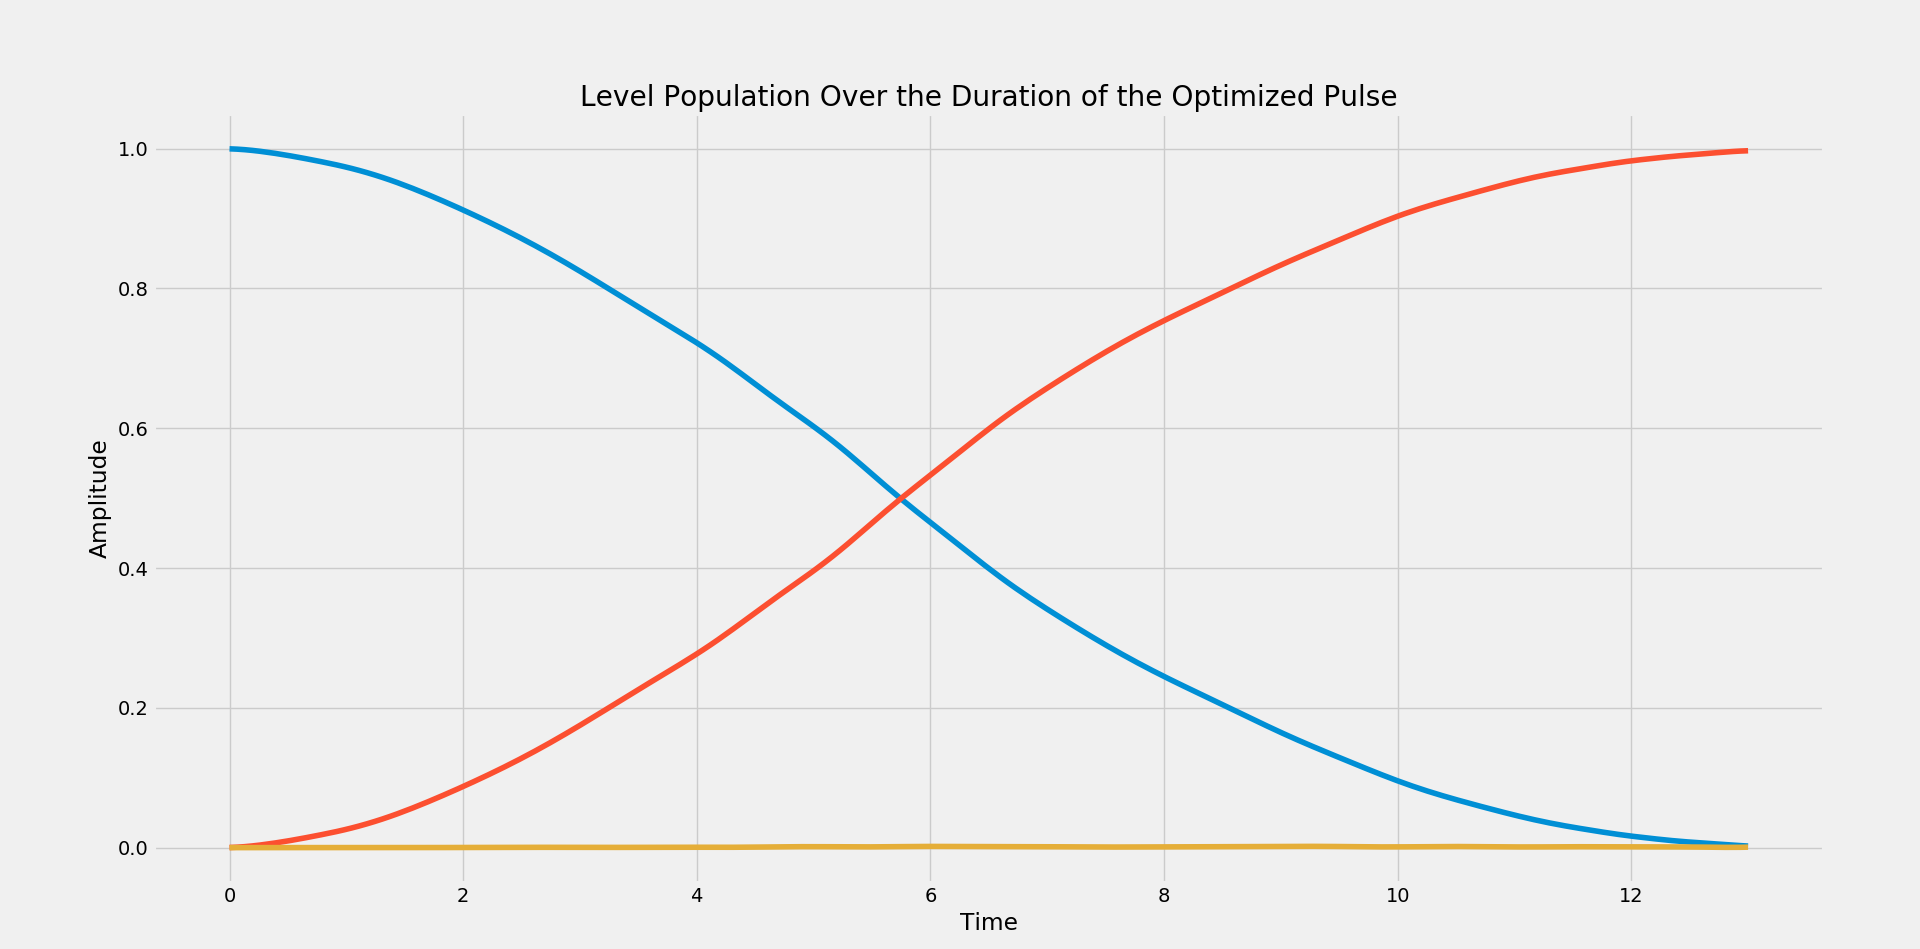
\includegraphics[width=1\columnwidth]{Results/DRAG/level-population2.png}
    \caption{Level population of the "qubit" over the duration of the pulse that was found by the GRAPE algorithm, with all the penalties turned on, including the DRAG penalty.}
    \label{fig:sDRAG-results}
\end{figure}
Nice! state $\ket{0}$ goes directly to $1$, $\ket{1}$ goes directly to $0$ and the forbidden level is barley changed throughout the pulse(the fidelity gotten from this pulse is around $99.9\%$, so pretty good).

I think that we talked enough about the qubit for now, let's move the the other half of the system, the cavity.


% TODO: Penalty on higher levels
% TODO: Definitely needs some rewording and expanding

% \subsection{Results and Pretty Graphs :)}
% \textit{Note: There is no quantum chip we can use to do the experiment, the result are of the numerical simulations.}
% \subsubsection{Preparing a Fock State in the Cavity}
% ...
% \subsubsection{Some Gates(?)}
% TODO: Should add some graphs here
\subsection{Implementing Cavity Operations}
\subsubsection{Limiting the photon number} 
\centerline{\say{Hilbert space is a big place.}}
\centerline{- Carlton Caves}
Here's the thing about the cavity levels, there are infinite amount of them. This might be a problem since our computers can't really deal with infinite amount that well. We can make an assumption that the cavity only has \(N\) levels but it is still possible that something happens in the higher levels that may affect the physical result that we didn't include in the simulation. We want to limit that and make sure that everything interesting is contained in the \(N\) levels that we have.

This is quiet similar to what we did in the previous section, we want to put a penalty on the higher levels, still, there are two main differences. The first, is that there are much more then one or two extra levels, and as we've seen, the method we used in the previous uses very heavy computation and we can't do it for so many levels since we want our computer to not explode. The other difference is that care less about if some higher level is occupied for a part of the pulse, in the cavity there are higher levels and they're all likely to be but \textbf{the reason we're limiting the cavity levels is for computing reasons, not physical ones}. Unlike the cavity, we really want the qubit to have only two levels and the only reason we simulate the higher ones is because the physical world is not as fun as the mathematical one and we can't simply ignore the higher levels. So it makes sense that we'll use a different penalty to limit the photon number. Let's take a look on how we'll do so. 

The idea is this, we'll define $n_{ph}$ as the highest level we want the cavity to have, now let's calculate what will happen if the cavity will have another level, for a total of $n_{ph} + 1$. Ideally, nothing will change, the new level should start at 0 probability and end at 0 probability with no change in between, if there is a change, will add a penalty to the pulse, so in the next iteration there will be less of a change. We can do so for and level higher then $1$, so instead of using only $n_{ph} + 1$ we'll some over $n_{ph} + k$ for reasonable amount of k's.

We'll define $F_{n_{ph} + k}$ as the fidelity if there were $n_{ph} + k$ levels. Putting the idea into a formula we get that the new cost function is given by
\[
    Cost = \sum_{k=0}^{N} F_{n_{ph} + k} (\vec{\epsilon}) - \sum_i \lambda_i g_i (\vec{\epsilon})
\]
We can double enforce the penalty if we add a constraing making sure there is no change in the fidelity for different levels
\[
    g_{ph} = \sum_{k_1 \ne k_2} (F_{n_{ph} + k_1} - F_{n_{ph} + k_2})^2
\]
The gradient of which is simply the gradient of which is simply
\[
    \frac{\partial g_{ph}}{\partial \epsilon_k} = 2 \sum_{k_1 \ne k_2} [(F_{n_{ph} + k_1} - F_{n_{ph} + k_2})(\frac{\partial F_{n_{ph} + k_1}}{\partial \epsilon_k} - \frac{\partial F_{n_{ph} + k_2}}{\partial \epsilon_k})]
\]
and everything in this expression was previously calculated(they're simply the derivatives of the fidelity and the fidelity itself).

It's important to note that while it might be tempting to leave $n_{ph}$ at a small value so there will be less to calculate(the size of the matrices grows with $n_{ph}^2$), there is good reason to use a high values of $n_{ph}$. Bigger $n_{ph}$ oscillate at higher frequency(since the cavity is simply a harmonic oscillator), so it's possible to use shorter pulses, and since keeping qubit alive is really a major problem, keeping the pulses short is important to be able to accomplish the most with the time we have with the qubit before it dies.
% TODO: Need to go over the last paragraph and check it with Serge to make sure I'm not making anything up

Lets see what happens if we run the transmon-cavity code. We'll only look at the resulting population graph after the optimization. I warn you that the graph is a bit cluttered. You shouldn't look at any specific details or any specific curve, I didn't put a legend explaining what each curve is. We'll look at it then discuess
% that there are 14 different curves, each curve represent a transmon-cavity state, they are colored differently and you can distinguish between them using the legend on the graph. We are going to run the example that does the state transfer $\ket{g} \otimes \ket{0} \quad \rightarrow \quad \ket{g} \otimes \ket{1}$, simply creating a photon in the cavity
\begin{figure}[H] % TODO: Change to correct picture
    \centering
    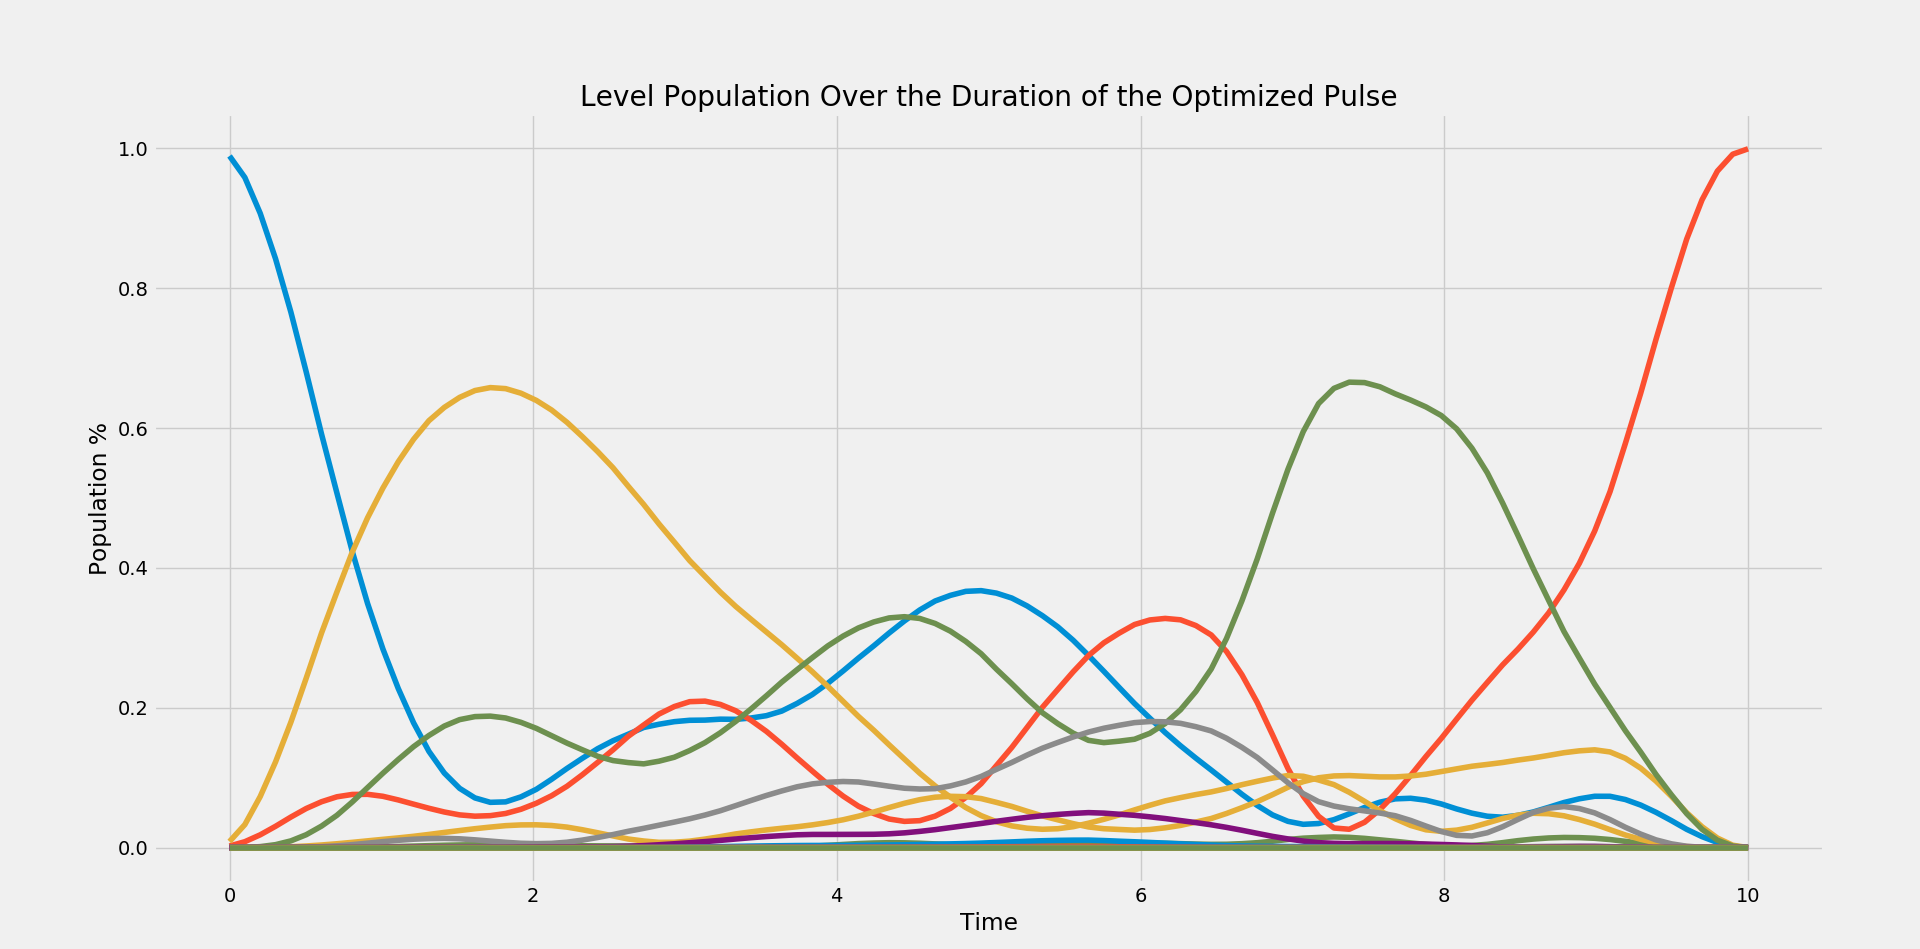
\includegraphics[width=1\columnwidth]{Results/transmon-cavity/g0-g1-level-population.png}
    \caption{Transmon-cavity state population over the duration of the pulse that does the transformation $\ket{g} \otimes \ket{0} \quad \rightarrow \quad \ket{g} \otimes \ket{1}$.}
    \label{fig:transmon-cavity-population}
\end{figure}
After you see this graph, you'd think that it didn't work correctly since the transformation is from one level to it's neighbor but there were too many levels that got occupied, this is a valid thing to think but one thing you need to know is that you can't really create number states directly in a cavity without exciting the higher levels, this is because you can only create directly coherent states, and what you need to do is make all the coherent states interfere in a way that creates a number state.

So why then should this graph show it was successful then? Well, I run the algorithm with 50 cavity levels(!), this means that there are actually 100 curves in that graph(50 of the cavity times 2 of the qubit). If you'd try to count the number of curves that you see you'll probably count 7-8 curves and not all of the 100, this is since most of the curves stay at zero population. This is exactly what we want, the higher levels don't affect the physics of the system, if we add more levels(like in the real world where there are infinte levels) the pulse would still give the same desired result.
% As you can see, although the final result is what we want it to be, along the way higher levels were created, even to last level of the cavity were excited. This is a problem since, as we said earlier, the cavity should have infinite levels and cutting it off after 7 levels in this case is just and approximation, the last levels should not be populated.

% We can now add the penalty and see that this problem is solved with it.

\subsection{Finding a Good Initial Guess}
Although the GRAPE algorithm is the one responsible to find to optimal control pulse, we still need to give it some initial guess and the algorithm does the rest. You might think that this isn't much of a problem since theoretically any initial guess should arrive at a desired result. The problem is that many times the algorithm gets stuck and can't find a result. This could be caused by a number of reasons, the main two are when the constraints are too strong and when the initial guess is not good enough.

When the constraints are two strong, the algorithm might prefer optimizing them instead of the fidelity and what we get is a pulse that achieves horrible fidelity but within the constraints. This is really not good and the solution is simply weakening the constraints(choosing a smaller $\lambda$ for the constraint).

The other, harder to solve problem is when the initial guess of the pulse is problematic. For example, if you choose the initial guess the be the most obvious initial guess you can make, constant 0, the algorithm will properly stop after one iteration changing nothing, this is because the gradient of a constant 0 pulse is actually zero, so the optimization algorithm think it's in an optimized minimum when in fact, it properly couldn't be more wrong.

The other simple initial guess you might think of using is a random pulse, after all we don't know what is the desired pulse so picking a random pulse is as good as any other, plus it has the added benefit that even if one random pulse doesn't get you to a solution, the next time you run it it might get to one. The problem with a random pulse is that it is the definition of a non-smooth function, and since the initial guess is not smooth, the algorithm might find it difficult to get a smooth solution.

There are two approaches we can take to get a good initial pulse, the first approach assumes nothing about the system, this is good since it is really general and can be used in any case, but might be not ideal in some cases. The second approach is when we know roughly how the solution should look like, we can use some pulse that is similar to what we expect and GRAPE will get the actual pulse from that.

In the first approach, we want GRAPE to do most of the work, but not get stuck by some weird problem of the initial pulse, we want a guess that is close to 0, pretty random, but not so much that it would be hard to smooth. We can get such a pulse by doing a \textit{convolution} between a random pulse and a Gaussian window % TODO: Continue to expalian why these convolutions work and give and equation

Unlike the first approach, the second approach could look really different for different examples but I'll give some general guidelines you can use the get a good initial pulse. Let's say, for example, you have a 3-level system where the third level isn't wanted(such as in the DRAG example). If you give an initial guess like the one in the first approach, the third level will still be excited by that pulse, and it might be hard for the algorithm to fix this. What you might do in this scenario, is to start with an initial guess that you know excites only the first and second levels of the system but not the third. This is easy since you  know the energy difference between the levels, and from that you know the frequency that excites each level. What you can do is some random pulse that has frequency around the first-second levels frequency difference. So if you look in the frequency space, what you see is some Gaussian distribution around the first levels frequency with some random noise on it.

\begin{figure}[H]
    \centering
    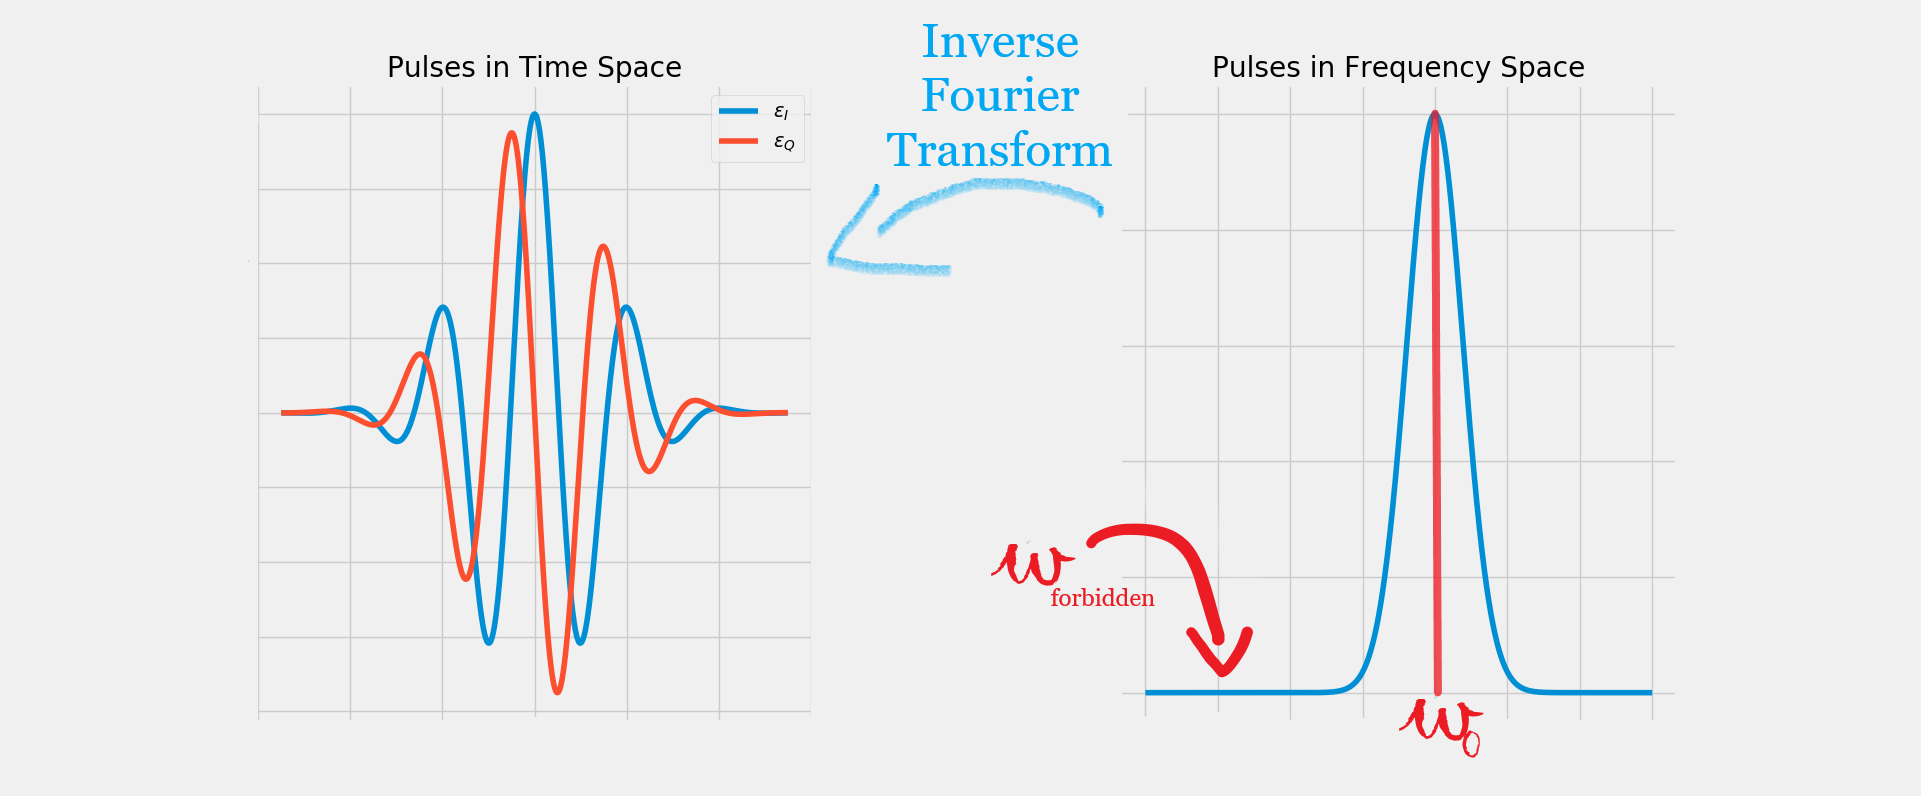
\includegraphics[width=1\columnwidth]{exaple-of-engineered-guess-edited.png}
    \caption{Example of how you might engineer an initial pulse for a system with known characteristics. Normally you would also add some random noise on top of the pulse}
    \label{fig:example-engineered-initial-guess}
\end{figure}
\subsection{From States to Gates}\label{sec:gate-GRAPE}
% TODO: Explain how you would go from state-GRAPE to gate-GRAPE and maybe implement it?
% \textit{*Maybe add here how to create a gate-GRAPE from the state-GRAPE*}
Until now we've discussed how to find pulses that take our system from one state to another. Which raises an important question, \textit{\textbf{why}?}. Sure, creating Fock states in cavity is nice and all, but I want to run quantum algorithm on my quantum computer not make pretty pictures.

Here's the thing, turns out, you can change the algorithm just a little bit and get a GRAPE algorithm that gives you back the optimal pulses that realizes a desired \textit{quantum gate}, instead of just taking you from one state to another. 

To make such gate GRAPE, instead of optimizing for one state transformation, you optimize for of initial states. These initial states should constitute a basis for the entire state space. This way, since quantum operations must be unitary, a unique transformation on the basis of the state space is a unique transformation on the entire system. We're no going to prove this I would not implement this or go any further, this is just a brief overview to get the general idea but I don't want to make this project too long.

\subsection{References and Further Readings}
...

\newpage
\section{Controlling a Superconducting Quantum Computer} \label{chap:FPGA}
\subsection{Overview}
Before jumping into the specifics of how'd we control the quantum computer, let's start with a general overview and show how everything is connected and the purpose of it all.

% As you might have noticed by now, our goal is to control a quantum computer.
% TODO: Continue
We'll start with a diagram that shows how the system is connected, from the pulse generator to the cavity.

\begin{figure}[H]
    \centering
    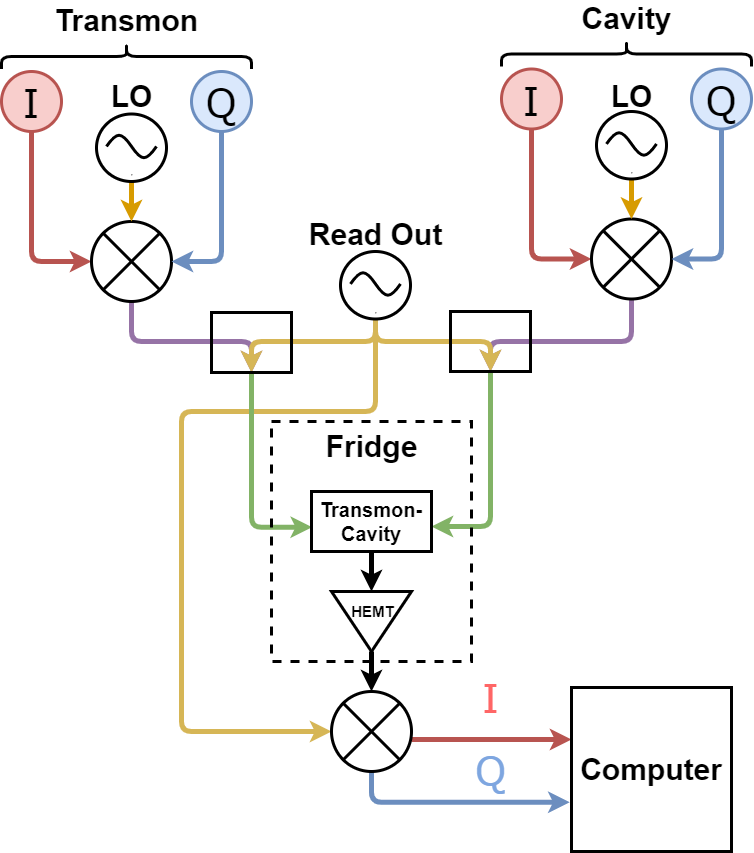
\includegraphics[width=0.8\columnwidth]{system-diagram.png}
    \caption{Diagram of the system}
    \label{fig:System-diagram}
\end{figure}

The $I$ and $Q$ signals are generated in the AWG, the LO frequency comes from a frequency generator and so does the Read Out signal. HEMT is a signal amplifier. I talk much more on each component in this chapter, this is just a diagram to so you'd be able to relate each component we talk about the where it is in the system.

\subsection{Generating the Pulses}
\subsubsection{The AWG}
It shouldn't be too much of a surprise if I'll tell you that I consider the AWG(Arbitrary Waveform Generator) the "heart\ensuremath\heartsuit" of the system, we've just spent an entire chapter on finding the pulses we want to send, and the instrument that creates and sends the pulse, is the AWG. Unfortunately, using the AWG isn't as straight-forward as you might hope and there are some problem's we'll need to address if we want our system to work.

Consider for a moment what we want to do with our microwave generator to control a qubit, we need to send a high frequency signal and change it by a really small amount compared to its frequency(sending a GHz signal and changing it by MHz, 3 orders of magnitude difference). We can't just take a wave generator that generates a 10GHz signal and tell it to change from 10GHz to 10.0001GHz because it won't be precise enough, and even if the frequency generator is good enough so that we can make really accurate changes to the frequency, we still want to have the wave interact with the quantum system and analyze the result so we also need a super-frequency-analyzer to understand what the hell is going on in the quantum system, not only that, we also want the frequency analyzer and generator to work together(matching the same input with the corresponding output of the system). Now that we understand what are some of the challenges working with such high frequencies, what can we do about it?

Well the solution is simple, we can take a high frequency wave(10GHz for example) and a lower frequency wave(1MHz for example) and mix them together \textit{somehow} to get a $10\text{GHz} + 1\text{MHz} = 10.0001\text{GHz}$ signal, and in the output of the quantum system we can simply un-mix the result to get back the 10GHz signal and some other signal(in the MHz) that can tell us something about the system.

That sounds all nice and good but how do we actually mix/un-mix 2 signals in that way and how can we control that proccess? That's where the IO-Mixer comes in, we'll look into them in just a moment, first we need to understand a regular mixer work.

\subsubsection{The Mixer}
The idea is simple, the mixer has 2 inputs and one output, when you enter 2 waves as an input, you get their product as the output(inputting for example $\cos(t)$ and $\cos(2t)$ will result in $\cos(t)cos(2t)$ at the output). % We look more into mixers, couplers and their implementation in appendix \ref{appen:Mixers}.
% TODO: Maybe add here more about couplers instead of in an appendix
We draw a mixer in a diagram like so,

\begin{figure}[H]
    \centering
    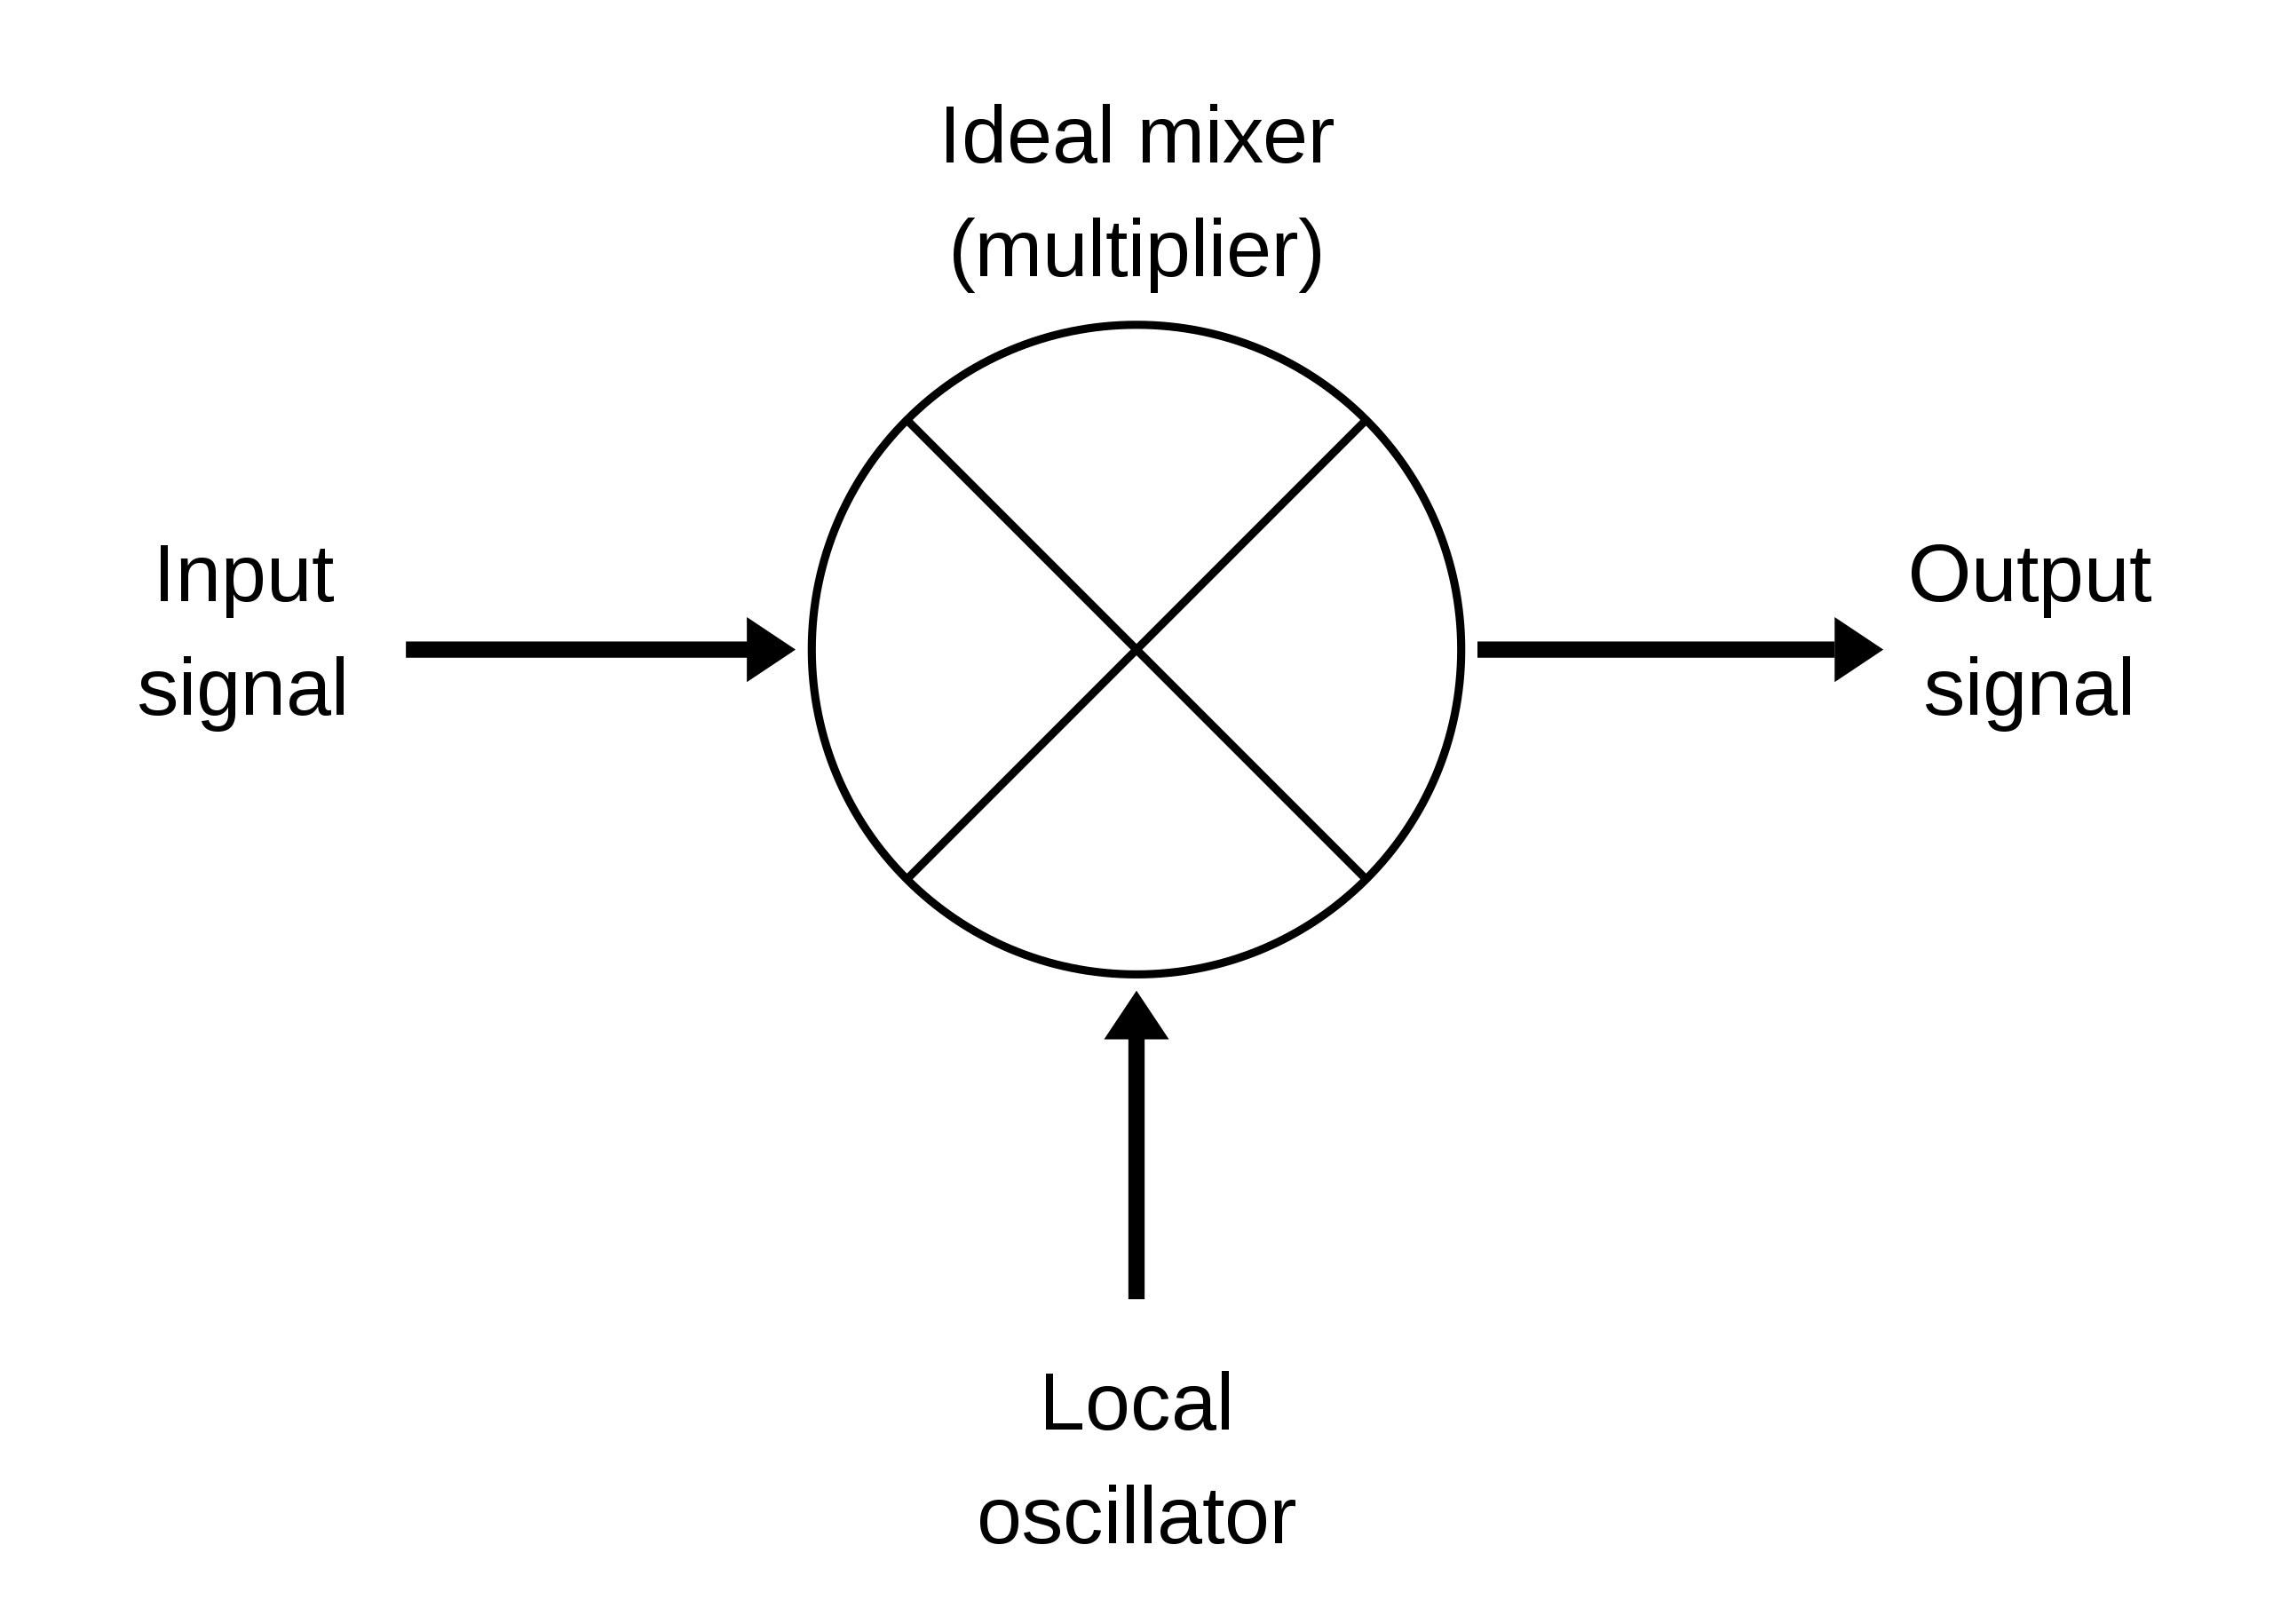
\includegraphics[width=0.3\columnwidth]{Ideal-Mixer.png} %TODO: Change image to one with L I R markings
    \caption{Ideal mixer in a diagram}
    \label{fig:Ideal-Mixer}
\end{figure}
We can change what are the outputs and what are the inputs to get different ways for the mixer to work\footnote{TODO: Explain this} % TODO: Add on this later

\subsubsection{The IQ-Mixer}
% Marki website - sent on mail
We've seen what's a \textit{regular}(and \textit{ideal}) mixer is, but how can we use it for the desired effect? remember, we want to input a high frequency and a lower frequency and we want the output to be a wave with a frequency that is the sum of the 2 frequencies. To do so, we can consider the following diagram
\begin{figure}[H]
    \centering
    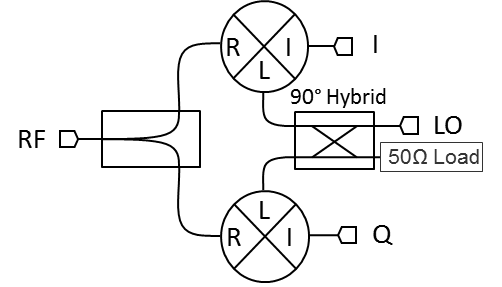
\includegraphics[width=0.5\columnwidth]{IQ-Mixer.png} %TODO: Change image to one with L I R markings
    \caption{The IQ mixer}
    \label{fig:IQ-Mixer}
\end{figure}
Where the 90\degree\ hybrid in the diagram is a \textit{90\degree\  hybrid coupler}, it splits the signal into 2 signals at a 90\degree phase difference, hence the name. The square near the \textit{RF} sign simply adds the 2 waves, we also look into it in the appendix % TODO: Improve wording
% TODO: 90 Degree hybrid explenation instead of in the appendix

As we can see, the IQ mixer has 3 inputs, \textit{I}, \textit{Q}(hence the name) and \textit{LO}. We can also see that there's only one output, \textit{RF}(although you can play with what are the inputs and what are the outputs).

How can we use this IQ mixer to add frequencies? Let's consider the following inputs\footnote{You can flip I and Q and get subtraction instead of addition}
\begin{align*}
    I &---> \cos(\omega_{IQ} t)\\
    Q &---> \sin(\omega_{IQ} t)\\
    LO &---> \sin(\omega_{LO}t)
\end{align*}
In this case, the input into the top mixer will be \textit{I} and a \textit{LO}, which is $\cos(\omega_{IQ}t)\sin(\omega_{LO}t)$. Similarly, the input into the bottom mixer will be \textit{Q} and 90\degree phase of \textit{LO}, which is $\sin(\omega_{IQ}t)\cos(\omega_{LO}t)$.

The total output(in \textit{RF}) will be the sum of the two waves
$$RF = \cos(\omega_{IQ}t)\sin(\omega_{LO}t) + \sin(\omega_{IQ}t)\cos(\omega_{LO}t)$$
and we know from simple trigonometry that $sin(a + b) = \cos(a)\sin(b) + \sin(a)\cos(b)$, so we get
\begin{equation}
    \boxed{RF = \sin((\omega_{LO} + \omega_{IQ})t)}
\end{equation}

Perfect! this is exactly what we wanted, the output is a wave with frequency that is the some of the input frequencies. Only one problem, it doesn't work :(.

\subsubsection{Theory VS Reality :(} % Maybe combine this section and the next one
If we use a spectrum analyzer and view what frequencies are in the final wave we get the following picture

\begin{figure}[H]
    \centering
    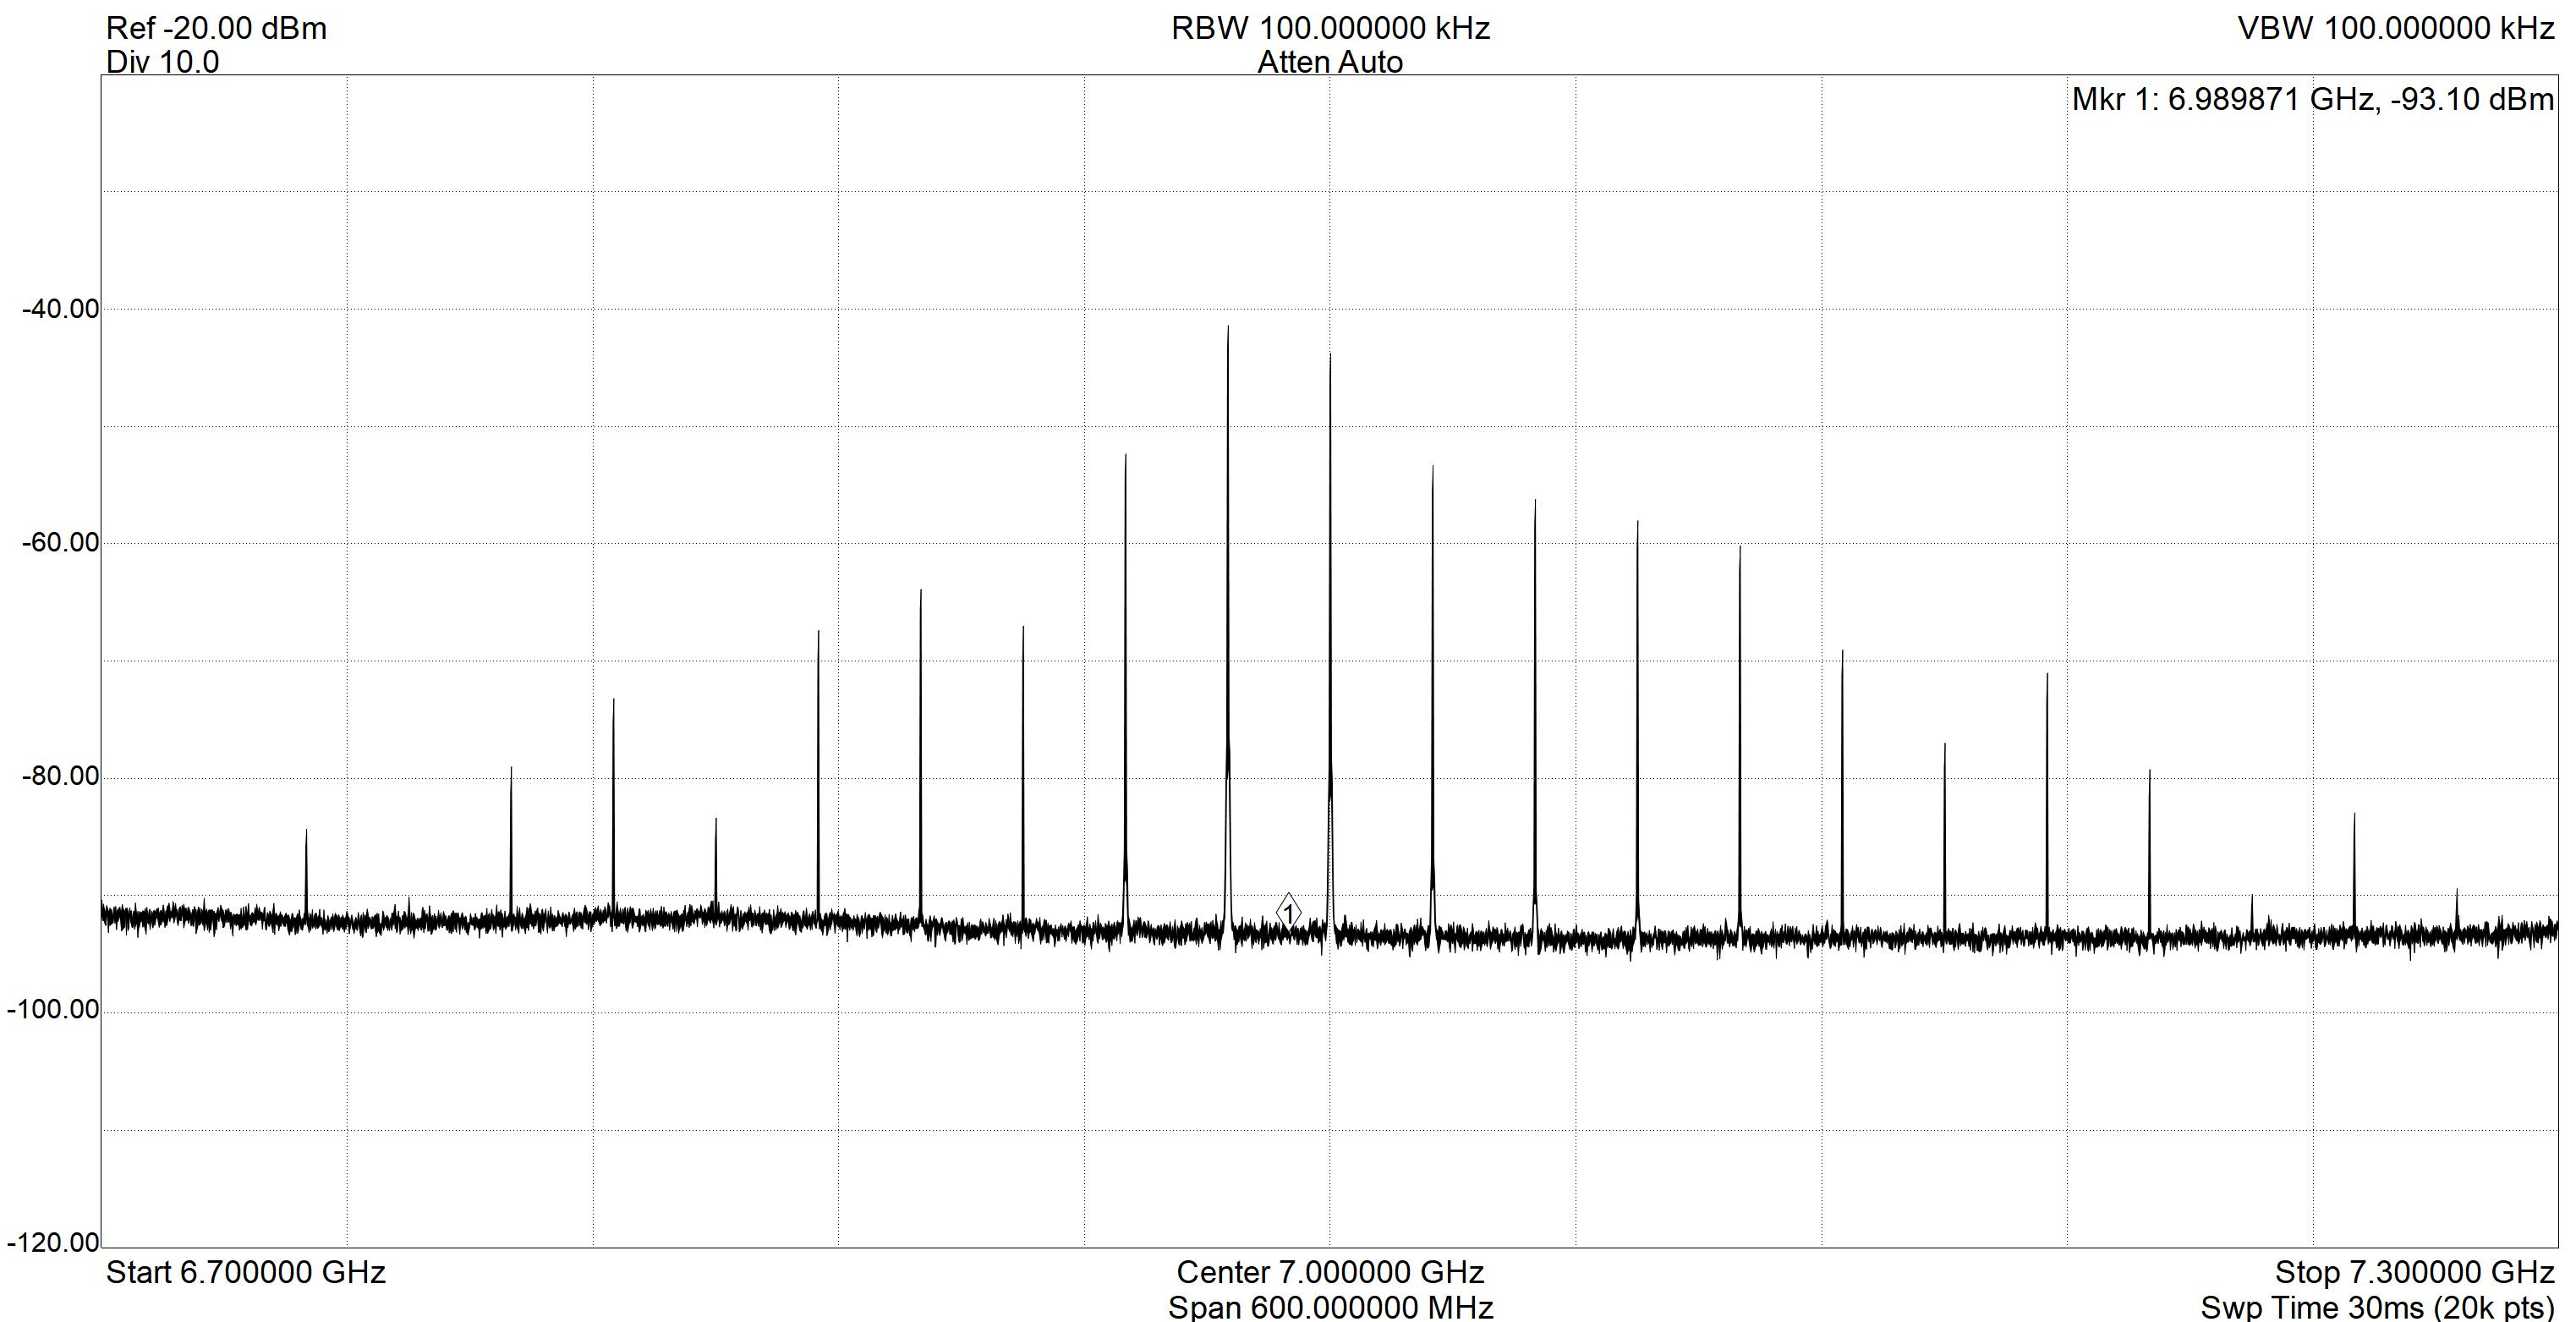
\includegraphics[width=0.8\columnwidth]{full-spectrum-no-correction.jpg} %TODO: Need to change to image with explantion on what is going on
    \caption{Full Spectrum Without Any Corrections}
    \label{fig:Full-spectrum-no-corrections}
\end{figure}
Zooming in around the LO frequency we see
\begin{figure}[H]
    \centering
    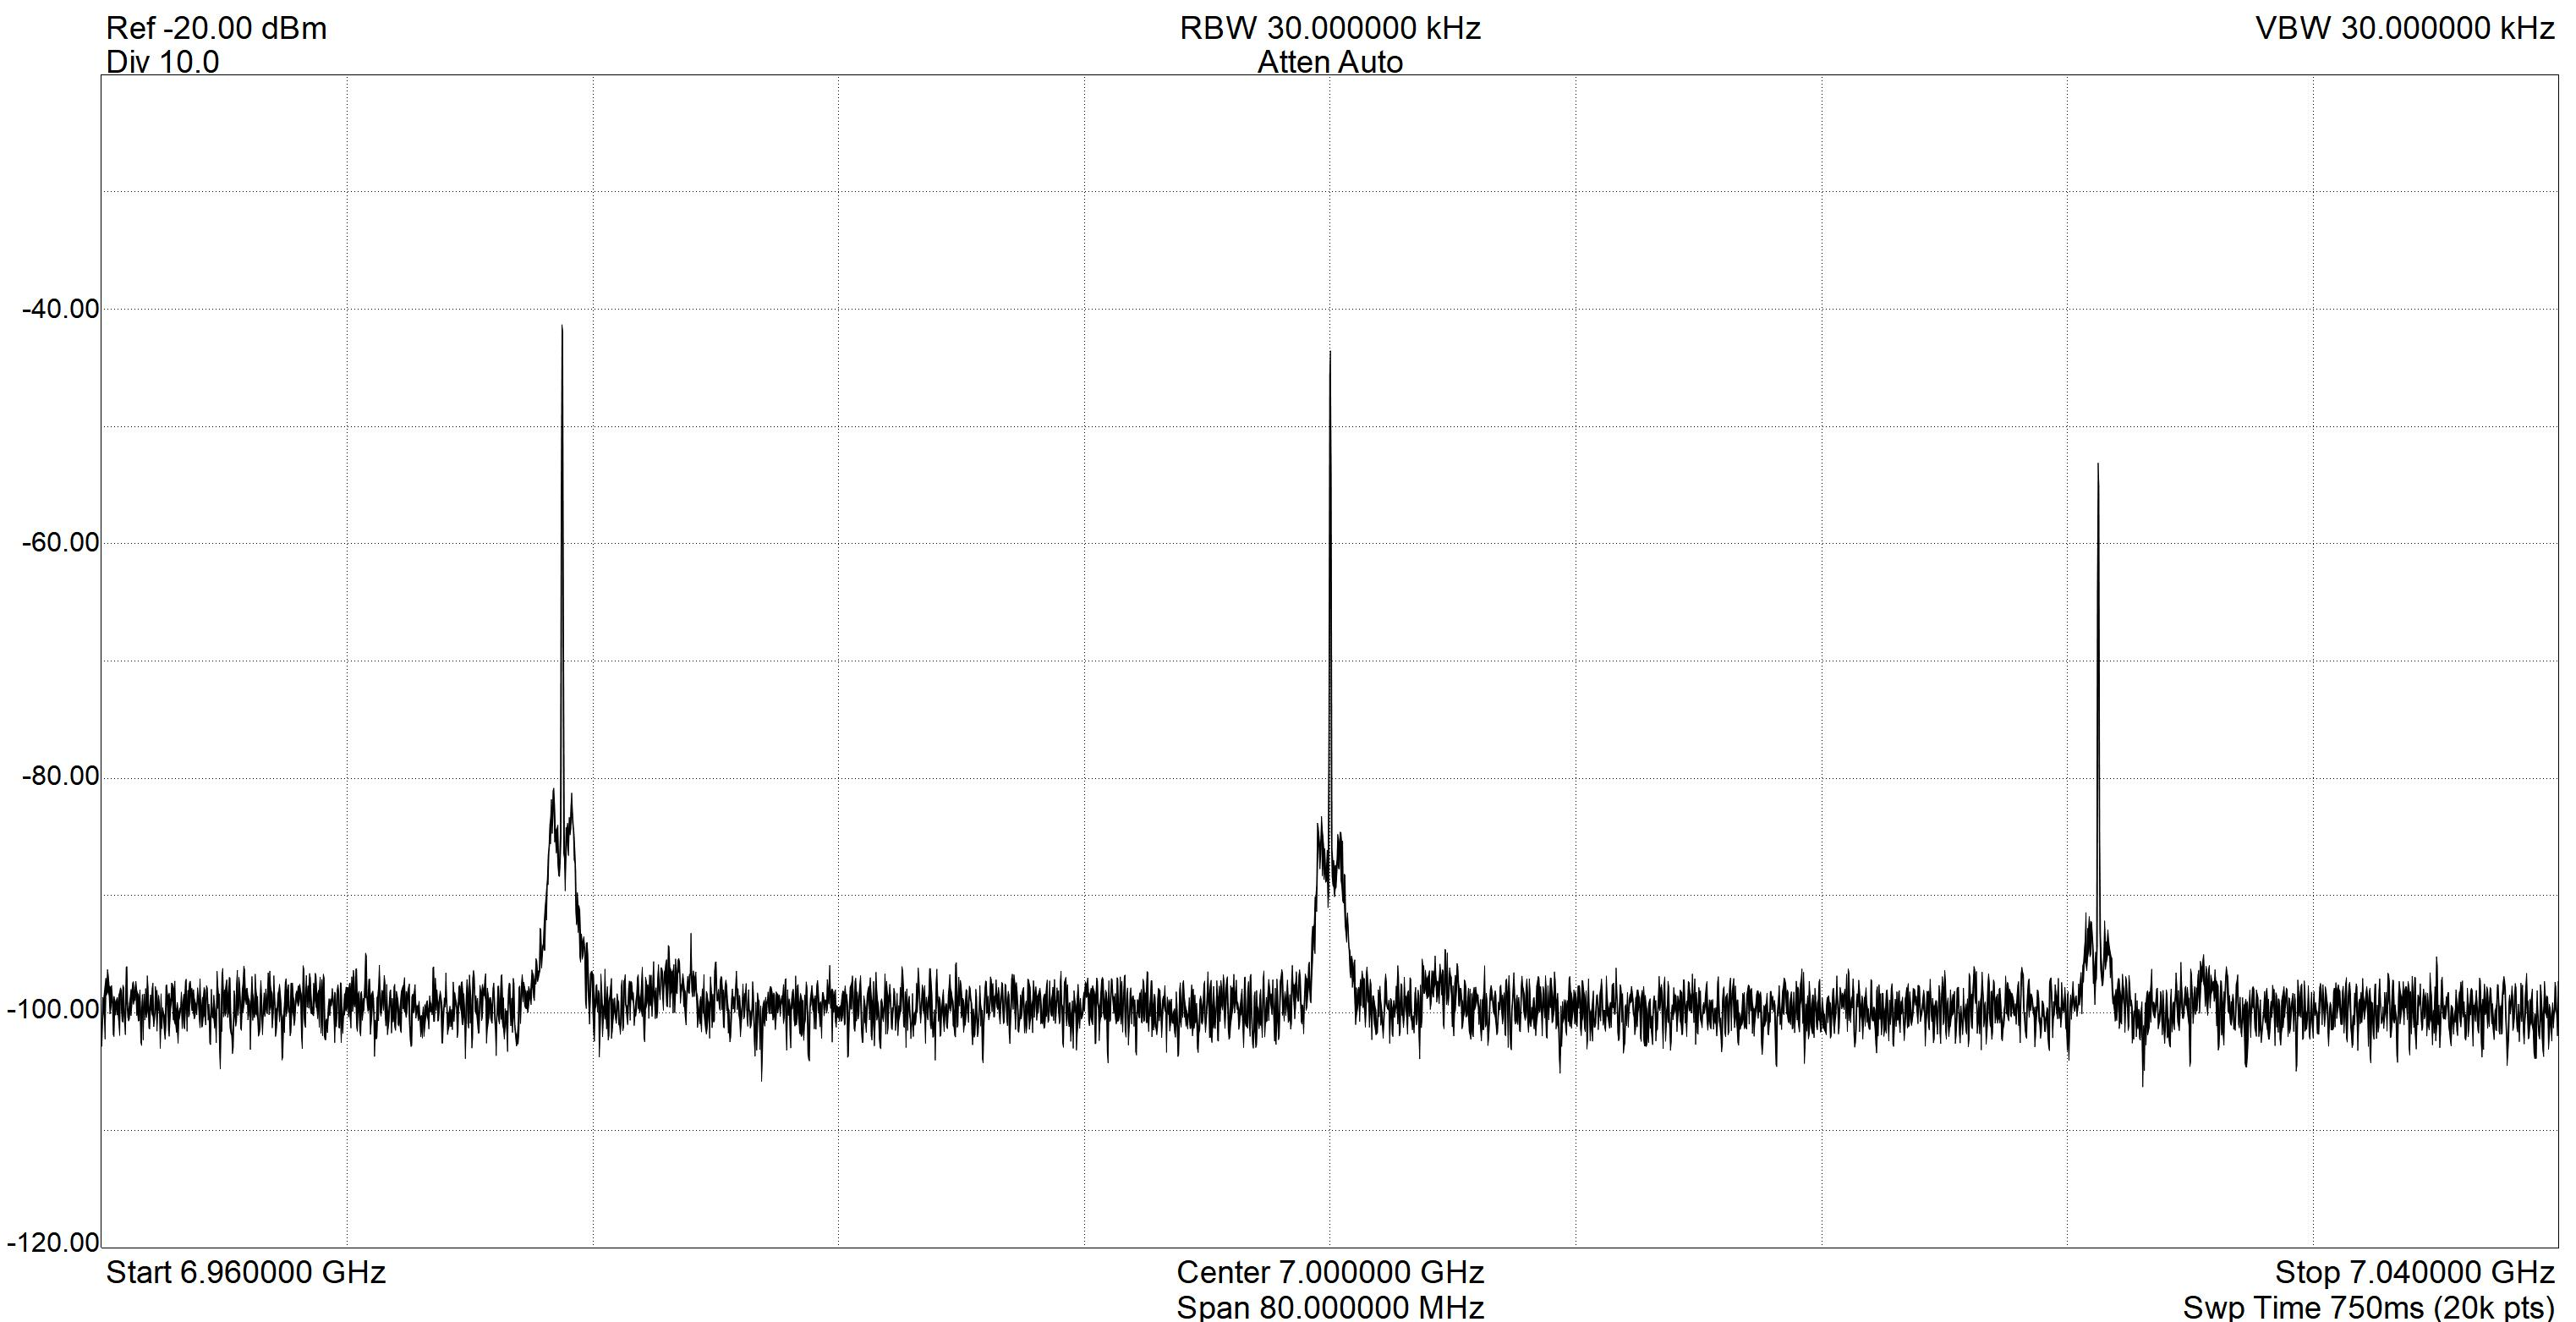
\includegraphics[width=0.8\columnwidth]{Important-Spectrum-no-correction.jpg} %TODO: Need to change the image to one with marking explaining it on it(what is each spike)
    \caption{Spectrum Around the LO Frequency}
    \label{fig:closeup-spectrum-no-corrections}
\end{figure}

What is the problem? We've proved mathematically that it should work, so why doesn't it? The problem is that we can't just assume the waves to come and go with the same phase, the waves travel through the wire at some speed so if we input into two different wires, two waves that are at the same phase, at the other side of the wire they might come at different phases because of differences in wire length, resistance, etc... So what can we do about it? You could try to make identical parts and make everything just perfect but even slight deviation will cause the system no to work properly, a better solution is to input more complex waves and have some parameters to play with so we can simply find the right parameters for the system and then it will work.% TODO: Improve wording

We can analyze the frequency space of the output of out IQ mixer and we can see 2 types of it not working correctly
\begin{itemize}
  \item Leakage at the LO frequency
  \item Leakage at \(\omega_LO - \omega_IQ\)
\end{itemize}
We can solve the first type of Leakage, at the LO frequency, by adding DC offsets to the input frequencies(We'll prove this mathematically later), and we can solve the second type of leakage by adding phase offsets to the waves(We'll prove this mathematically later).
% This is how the frequency spectrum looks without making any changes to the input waves
%TODO: Add frequency space figure without any corrections.
\subsubsection{Solution for the real world} \label{sec:solution_real_world}
Before we can solve the problem, we need to understand what's causing it. As we explained earlier, a phase  is created  in the wires that connect everything.
\paragraph*{Leakage at \(\omega_{LO} - \omega_{IQ}\) }
% \subsection{What's causing the problem}
Let's consider now inputting into the IQ mixer the same waves but with the phases that were created in the transmission wires instead of what we had earlier
\begin{align*}
    I &---> \cos(\omega_{IQ} t + \phi_I) \\% + \epsilon_I\\
    Q &---> \sin(\omega_{IQ} t + \phi_Q) \\% + \epsilon_Q\\
    LO &---> \sin(\omega_{LO}t + \phi_{LO})
\end{align*}
Using the same calculation we did before, we get that
$$RF = I\cdot LO + Q\cdot LO(90\degree)$$
\[
RF = \cos(\omega_{IQ} t + \phi_I) \cdot \sin(\omega_{LO}t + \phi_{LO}) + \sin(\omega_{IQ} t + \phi_Q) \cdot \cos(\omega_{LO}t + \phi_{LO}) 
\]
If you can trust me on the algebra(or rather, trust wolfram alpha on the algebra...) we get the expression
\begin{align*}
RF = &\cos(\frac{\phi_Q - \phi_I}{2})\sin((\omega_{IQ} + \omega_{LO})t + \frac{\phi_Q + \phi_I}{2} + \phi_{LO}) \\
   + &\sin(\frac{\phi_Q - \phi_I}{2})\cos((\omega_{IQ} - \omega_{LO})t + \frac{\phi_Q + \phi_I}{2} - \phi_{LO})
\end{align*}
This expression is quiet scarier than the one we got earlier... More than that, we get two frequencies instead of one, we've got an unwanted frequency at \(\omega_{LO} - \omega_{IQ}\) and the only way to make it disappear is if the phases are equal, \(\phi_I = \phi_Q\). Also the final wave as a phase of \(\phi_{LO}\), this isn't really a problem and if we define our starting point differently we can set  \(\phi_{LO}\) to 0.

\paragraph*{LO Frequency Leakage}
% TODO: Maybe I'll be able to find a mathematicall explenation to the DC offsets
Another type of leakage we've observed is leakage at the LO frequency, it makes sense that some of the original wave will go through the mixer untouched. To fix that leakage, we'll need to somehow change the I and Q waves to cancel it out. The simplest way to do so is to add DC offsets to the inputs \footnote{I've removed the phase on the LO wave since we've seen it doesn't really change anything}
\begin{align*}
    I &---> \cos(\omega_{IQ} t + \phi_I) + \epsilon_I\\
    Q &---> \sin(\omega_{IQ} t + \phi_Q) + \epsilon_Q\\
    LO &---> \sin(\omega_{LO}t)
\end{align*}
We've seen this story before... the calculation of the RF wave is the same so we'll skip the calculation. The end result is
\begin{align*}
RF = &\cos(\frac{\phi_Q - \phi_I}{2})\sin((\omega_{IQ} + \omega_{LO})t + \frac{\phi_Q + \phi_I}{2}) \\
   + &\sin(\frac{\phi_Q - \phi_I}{2})\cos((\omega_{IQ} - \omega_{LO})t + \frac{\phi_Q + \phi_I}{2}) \\
   + &\epsilon_I  \sin(\omega_{LO}t) + \epsilon_Q  \cos(\omega_{LO}t) \\
   = &RF_{old} + \epsilon_I  \sin(\omega_{LO}t) + \epsilon_Q  \cos(\omega_{LO}t)
\end{align*}
where \(RF_{old}\) is the RF wave before adding the DC offsets. 

What we get is the same wave, but now we can play with the LO frequency at the output. Later we'll change the DC offsets so that they will cancel to LO frequency leakage to minimize it.

Now that we have all of our "knobs" we can change and play with, we can start using them to minimize the leakages.


\subsubsection{Finding Optimal Constants} % Maybe I won't do this section
As we've seen in the previous section, there are 4 variables we can "play" with to get the best variables for our system, as long as we don't change the system, these variables stay the same. What we want to do now is to actually find them. Our system is connected like so
% Add figure of how the system is connected

We have the Quantum Machine\footnote{this is the heart of the system, for now we'll use it to make the MHz waves with different phases, DC offsets and frequencies} that generates the I and Q inputs that go into the mixer(and also to an oscilloscope for debugging). There's the frequency generator\footnote{KeySight N5173B} that is connected to the mixer and generates 7GHz wave, and there's the frequency spectrum analyzer\footnote{SignalHound USB SA-124B} that is connected to the computer.

Let's first attack the leakage at the LO frequency. For now we'll have an LO frequency of 7GHz that we want to change by 25MHz(The same variables work for all frequencies this is just as an example)

\paragraph{LO frequency Leakage}
As proven in section \ref{sec:solution_real_world}, to minimize this kind of leakage all we need is to play with the DC offsets of the IQ inputs. To do so, we first need to define what we want to minimize, which in this case is simply the power of the frequency at 7GHz, we can measure that power with our spectrum analyzer, we'll call that our \textit{cost function}.
We have a 2-dimensional variable space, we need to find where in this space the cost function is at a minimum. To do so, we'll start by using a brute force method to find the general location of the minimum in the variable space, since brute force is very inefficient we can't really use it to find the exact location of the minimum so we start by only doing a low precision brute force and then use a different optimization algorithm to find the exact location of the minimum. We'll use the \texttt{scipy.optimize.fmin} as the algorithm for precise minimum location.%\footnote{see more in appendix \ref{appen:opt}} % TODO: Improve wording
% TODO: Add figure of spectrum after leakage optimazation

\paragraph{Harmonies Leakage}
Now that we've minimized the LO frequency leakage, we want to minimize the harmony leakage, we do that by changing to phases of the IQ waves from the quantum machine, it's important that changing the phases doesn't change the LO leakage and luckily for us, as proven in section \ref{sec:solution_real_world} that's whats happening. to change the phases we don't simply specify the phases, we use the correction matrix of the Quantum Machine. % TODO: Add explanations about the correction matrix(scale on angle) 
This time our cost function is the frequency at $\omega_{LO} - \omega_{IQ}$, we can do the same as we did in the LO leakage and use first a brute force optimization to find the general location of the minimum and the use the fmin algorithm to find the exact location of the minimum of the cost function(this time in the scale-angle variable space). You can see the result here
% TODO: Add figure of full final optimization
% TODO: Explain why it doesn't work perfectly(The quantum machine power problem)
% \subsection{Some other problems maybe?}
% ...
\subsection{References and Further Readings}
...

\newpage
\section{Future Work and Conclusions}
We conclude this project with the knowledge and tools(both mental and literal python program utilities) to create and control quantum systems, from understanding them theoretically to connecting and calibrating the devices that actually send the control pulses, to creating the control pulses to create any quantum state we can think of and any operation we want.

As with anything in life, this project must to come to an end at some point, each subject we discuss opens a rabbit hole we'll never see the end of. Everything could be expanded and studied but we can't keep adding and adding to the project.

If I we're the continue this project, properly the first thing I would do is explain exactly how the gate GRAPE from section \ref{sec:gate-GRAPE} works, and implement it in code. The gate GRAPE is the missing piece needed to actually creating quantum circuits, and it opens many possibilities for quantum computation and information.

Another, pretty obvious, continuation to this project would be, you know, actually implementing it, physically, in an experiment. This project is (almost) entirely theoretical and numerical, for all you know I was lying to you the hole time. It would be nice to actually check GRAPE on quantum system, but since Serge's lab is not yet fully built and there is no fridge to cool the quantum system system to to be able to create stable quantum states, it is impossible to do the experiments needed. More then that, it would make the project much longer then it is right now, and we must finish it at some point.

 The last important addition I can add to the project is characterizing system of multiple qubits, this shouldn't be that difficult since the qubit-qubit(or atom-atom) interaction aren't that different from the qubit-cavity interaction we already have, and our optimal control code accepts quantum states in any Hilbert space so to only different would be some additional Hamiltonian terms of the qubit-qubit interaction and different initial and target states that include the multiple qubit situation(which from the introduction we know that it's simply the tensor product of the qubit states).

% TODO: Refine this and maybe add a thanking paragraph


\appendix
% \newpage
% \section{Quantum Optics}
% Most of the physics in this project comes in the form of \textit{quantum optics}, mainly, in the Jaynes-Cumming model that describes the qubit, the cavity, and the interaction between them. It is essential to know at least the basics of quantum optics to understand the system and why it works as a quantum computer. In this appendix I will give a brief introduction to the subject, enough to understand anything in this project.

% \subsection{The Quantization of the Electromagnetic Field}
% \subsection{Coherent States}
% \subsection{Atom-Field Interactions}

% \newpage
% \section{The Jaynes–Cummings Model}
% Our goal is to mathematically model the Hamiltonian of a system of a two-level atom interacting with a single quantized mode of an optical cavity's electromagnetic field. % TODO: Add details about the original paper by Edwin Jaynes and Fred Cummings
% \par
% First we'll divide the system into 3 parts, The atom(it can be other two-level quantum systems), the cavity(electromagnetic field with quantized modes) and the interaction between the atom and the cavity(an atom can emit a photon to the cavity and change it's electromagnetic field, or catch a photon from the cavity and go up an energy level).\par  % http://aliramadhan.me/files/jaynes-cummings-model.pdf
% Let's start with the cavity(we'll consider a one dimensional cavity for now).

% \subsection{Homogeneous Electromagnetic Wave Equation}
% Maxwell's equations in free space are:
% \begin{subequations}
%     \label{eq:optim}
%     \begin{align}
%         &\grad \cdot \textbf{E} = 0 \label{eq:Maxwell-1}\\
%         &\grad \cdot \textbf{B} = 0 \label{eq:Maxwell-2}\\
%         &\grad \cross \textbf{E} = \frac{\partial\textbf{B}}{\partial t} \label{eq:Maxwell-3}\\
%         &\grad \cross \textbf{B} = \mu_0 \epsilon_0 \frac{\partial\textbf{E}}{\partial t} \label{eq:Maxwell-4}
%     \end{align}
% \end{subequations}
% Taking the curl of \ref{eq:Maxwell-3} and \ref{eq:Maxwell-4} we get
% \begin{subequations} 
% \label{eq:curl-}
%     \begin{align}
%         &\curl{(\curl{\textbf{E}})} 
%         = \curl{(-\frac{\partial \textbf{B}}{\partial t})} 
%         = -\frac{\partial}{\partial t}(\curl{\textbf{B}})
%         = - \mu_0 \epsilon_0 \frac{\partial^2 E}{\partial t^2} 
%         \label{eq:curl-E}\\
%         &\curl{(\curl{\textbf{B}})} 
%         = \curl{(\mu_0 \epsilon_0 \frac{\partial E}{\partial t})} 
%         = \mu_0 \epsilon_0\frac{\partial}{\partial t}(\curl{E}) 
%         = - \mu_0 \epsilon_0 \frac{\partial^2 \textbf{B}}{\partial t^2} 
%         \label{eq:curl-B}
%     \end{align}
% \end{subequations}
   
% We can use the vector identity
% \begin{equation}
%     \nabla \times \left( \nabla \times \mathbf{V} \right) = \nabla \left( \nabla \cdot \mathbf{V} \right) - \nabla^2 \mathbf{V}
% \end{equation}
% And obtain from \ref{eq:curl-E} and \ref{eq:curl-B}
% \begin{subequations}
%     \begin{align}
%         &\nabla(\nabla \cdot \textbf{E}) - \nabla^2 \textbf{E} 
%         = -\mu_0\epsilon_0\frac{\partial^2 \textbf{E}}{\partial t^2} \\
%         &\nabla(\nabla \cdot \textbf{B}) - \nabla^2 \textbf{B} 
%         = -\mu_0\epsilon_0\frac{\partial^2 \textbf{B}}{\partial t^2}
%     \end{align}
% \end{subequations}
% Now, we can use \ref{eq:Maxwell-1} and \ref{eq:Maxwell-2} To cancel the left most term and get
% \begin{subequations}
%     \begin{align}
%         &\nabla^2 \textbf{E} = \mu_0\epsilon_0\frac{\partial^2 \textbf{E}}{\partial t^2}\\
%         &\nabla^2 \textbf{B} = \mu_0\epsilon_0\frac{\partial^2 \textbf{B}}{\partial t^2}
%     \end{align}
% \end{subequations}
% Now because we know that $v_{ph} = \frac{1}{\sqrt{\mu_0\epsilon_0}}$ and that the phase velocity of electromagnetic waves in a vacuum is the speed of light, $c_0$, we get
% \begin{equation} \label{eq:Homo_electro_wave}
%     \begin{split}
%         \nabla^2 \textbf{E} = \frac{1}{c_0^2}\frac{\partial^2 \textbf{E}}{\partial t^2} \\
%         \nabla^2 \textbf{B} = \frac{1}{c_0^2}\frac{\partial^2 \textbf{B}}{\partial t^2}
%     \end{split}
% \end{equation}
% % TODO: Check these equations with serge
% These equation are called \textit{the homogeneous electromagnetic wave equations}.
% We'll pick a polarization arbitrarily to be in the x direction(that way we get only the component of the electric field and the y component of the magnetic field, $E_x$ and $B_y$) so now we get,
% \begin{equation} \label{eq:Homo_electro_wave_pol}
%     \begin{split}
%         \frac{\partial^2 E_x}{\partial x^2} = \frac{1}{c_0^2}\frac{\partial^2 E_x}{\partial t^2} \\
%         \frac{\partial^2 B_y}{\partial y^2} = \frac{1}{c_0^2}\frac{\partial^2 B_y}{\partial t^2} 
%     \end{split}
% \end{equation}
% \subsection{The Hamiltonians}
% We want to separate the total Hamiltonian into approachable parts, we can separate it like so,
% \[
%     H = H_{atom} + H_{cavity} + H_{interaction}
% \]
% where the atom and cavity Hamiltonians are the Hamiltonian of the atom and cavity if they were the only part of the (closed)system and the interaction Hamiltonian is the Hamiltonian of the interaction between the atom and the cavity in the system.

% \subsubsection{cavity}

% We can easily solve \ref{eq:Homo_electro_wave_pol} using separation of variables,
% $$E_x(z, t)= Z(z)T(t)$$
% Yielding the solution,
% \begin{equation}
%     \begin{split}
%         E_x(z, t) = \sqrt{\frac{2 \omega_c^2}{V \epsilon_0}}q(t)\sin{kz} \\
%         B_y(z, t) = \sqrt{\frac{2 \mu_0}{V}}\dot{q}(t)\cos{kz}
%     \end{split}
% \end{equation}
% where $V$ is the effective volume of the cavity, $q$ is a time-dependent amplitude with units of length, and $k = m\pi/L$ for
% an integer $m > 0$

% The Hamiltonian is given by
% \begin{align}
%     H &= \frac{1}{2}\int\epsilon_0 \textbf{E}^2 + \frac{\textbf{B}^2}{\mu_0} dV \\
%     &= \frac{1}{2}\int\epsilon_0 E_x^2(z, t) + \frac{B_y^2(z, t)}{\mu_0} dz \\
%     &= \frac{1}{2}[\dot{q}^2(t) + \omega_c^2 q^2(t)]
% \end{align}
% This looks like the Hamiltonian of an harmonic oscillator.

% Now, going from dynamical variables to operators(considering $\dot{q} \equiv p$) we get,
% \begin{align}
%      &\hat{E}_x(z, t) = \sqrt{\frac{2 \omega_c^2}{V \epsilon_0}}\hat{q}(t)\sin{kz} \\
%      &\hat{B}_y(z, t) = \sqrt{\frac{2 \mu_0}{V}}\hat{p}(t)\cos{kz} \\
%      &\hat{H} = \frac{1}{2}[\hat{p}^2(t) + \omega_c^2 \hat{q}^2(t)]
% \end{align}

% Let’s introduce creation and annihilation operators,
% $$\hat{a}(t) = \frac{1}{\sqrt{2\hbar\omega_c}}[\omega_c\hat{q}(t) + i\hat{p}(t)]$$
% $$\hat{a}^\dag(t) = \frac{1}{\sqrt{2\hbar\omega_c}}[\omega_c\hat{q}(t) - i\hat{p}(t)]$$

% We can write the electric and magnetic field as,
% \begin{align}
%          &\hat{E}_x(   z, t) = E_0[\hat{a}(t) + \hat{a}^\dag(t)]\sin{kz} \\
%          &\hat{B}_y(z, t) = \frac{E_0}{c}[\hat{a}(t) - \hat{a}^\dag(t)]\cos{kz}
% \end{align}
% And we can write the Hamiltonian as,
% \begin{equation}
%     \boxed{\hat{H}_{cavity} = \hbar\omega_c[\hat{a}\hat{a}^\dag + \frac{1}{2}] \approx \hbar\omega_c\hat{a}\hat{a}^\dag}
% \end{equation}
% We can ignore the zero-point energy $\frac{\hbar\omega_c}{2}$ if we define it as the zero energy point.

% \subsubsection{atom}

% Now that we have the cavity's Hamiltonian, we can go on to calculate the atom(qubit) Hamiltonian. \newline
% Remember that the qubit is a 2-level system, meaning we can define it has a superposition of the ground, $\ket{g}$, and excited, $\ket{e}$, states. The energy of the atom is the sum of the energy of each state times it's energy($\sum E_sP(\ket{s})$). The probability to be in a state $\ket{s}$ is given by $\ket{s}\bra{s}$ so we can write,
% \begin{equation}
%     \hat{H}_{atom} = E_g\ket{g}\bra{g} + E_e\ket{e}\bra{e}
% \end{equation}
% Using the vector representation of these states we'll write,
% %\begin{equation}
%     \begin{align*} 
%         \hat{H}_{atom} &= 
%         E_e \begin{bmatrix}
%         1 & 0     \\
%         0   & 0   \\
%         \end{bmatrix}
%         + E_g \begin{bmatrix}
%         0 & 0     \\
%         0   & 1   \\
%         \end{bmatrix} = 
%         \begin{bmatrix}
%         E_e & 0     \\
%         0   & E_g   \\
%         \end{bmatrix} \\
%         &= \frac{1}{2}\begin{bmatrix}
%         E_g + E_e & 0          \\
%         0         & E_g + E_e  \\
%         \end{bmatrix} +
%         \frac{1}{2}\begin{bmatrix}
%         E_e - E_g & 0          \\
%         0         & -(E_e - E_g)  \\
%         \end{bmatrix} \\
%         &= \frac{1}{2}(E_g + E_e)\begin{bmatrix}
%         1 & 0          \\
%         0         & 1  \\
%         \end{bmatrix} +
%         \frac{1}{2}(E_e - E_g)\begin{bmatrix}
%         1 & 0          \\
%         0         & -1  \\
%         \end{bmatrix} \\
%         &= \frac{1}{2}(E_g + E_e)\mathbb{I} + \frac{1}{2}(E_e - E_g)\hat{\sigma}_z
%     \end{align*}
% %\end{equation}
% Again, we can define the zero point energy so that the first term becomes $0$. We know the difference between the excited state energy and the ground state energy because it's approximately an harmonic oscillator so $E_e - E_g = \hbar\omega_a$ where $\omega_a$ is the atom frequency. Now we can write,
% \begin{equation}
%     \boxed{\hat{H}_{atom} = \frac{1}{2}\hbar\omega_a\hat{\sigma}_z}
% \end{equation}

% \subsubsection{interaction}

% Now for the last part of the Hamiltonian, we want to know the interaction Hamiltonian between the atom and the cavity. The interaction Hamiltonian is now 
% \[
% \hat{H}_{interaction} = -\hat{\textbf{d}}\cdot\hat{\textbf{E}} = -\hat{d} E_0 \sin{kz} (\hat{a} + \hat{a}^\dag{})
% \]
% Where we introduced $\hat{d} = \hat{\textbf{d}} \cdot \hat{x}$ (remember that we defined the axis so that x is the direction of polarization of the electromagnetic field).
% We'll also introduce the atomic transition operators
% \[
%     \hat{\sigma}_+ = \ket{e}\bra{g}, \quad\quad \hat{\sigma}_- = \ket{g}\bra{e} = \hat{\sigma}_+^{\dag{}}
% \]
% and the inversion operator
% \[
% \hat{\sigma}_z = \ket{e}\bra{e} - \ket{g}\bra{g}
% \]
% only the off-diagonal elements of the dipole operator are nonzero so we may write
% \[
%     \hat{d} = d\ket{e}\bra{g} + d^* \ket{g}\bra{e} = d\hat{\sigma}_- + d^* \hat{\sigma}_+ = d(\hat{\sigma}_+ + \hat{\sigma}_-)
% \]
% thus the interaction Hamiltonian is
% \begin{equation}
%     \hat{H}_{interaction} = \hbar\lambda(\hat{\sigma}_+ + \hat{\sigma}_-)(\hat{a} +  \hat{a}^\dag) 
%     = \hbar\lambda(\hat{\sigma}_+\hat{a} + \hat{\sigma}_+\hat{a}^\dag + \hat{\sigma}_-\hat{a} + \hat{\sigma}_-\hat{a}^\dag) 
% \end{equation}
% We shown the the operators $\hat{a}$ and $\hat{a}^\dag{}$ evolve as
% \begin{equation}
%     \hat{a}(t) = \hat{a}(0)e^{-i\omega t}, \quad\quad \hat{a}^\dag{}(t) = \hat{a}^\dag{}(0)e^{i\omega t}
% \end{equation}
% And similarly we can show for the free-atomic case that
% \begin{equation}
%     \hat{\sigma}_{\pm}(t) =   \hat{\sigma}_{\pm}(0)e^{\pm i\omega t}
% \end{equation}
% We can write while approximating $\omega_0 \approx \omega$
% \begin{equation}
%     \begin{split}
%         &\hat{\sigma}_+\hat{a} \sim e^{i(\omega_0 - \omega)t}\\
%         &\hat{\sigma}_-\hat{a}^\dag \sim e^{-i(\omega_0 - \omega)t}\\
%         &\hat{\sigma}_+\hat{a}^\dag \sim e^{i(\omega_0 + \omega)t}\\
%         &\hat{\sigma}_-\hat{a} \sim e^{-i(\omega_0 + \omega)t}
%     \end{split}
% \end{equation}
% We can see that the last two term vary much more rapidly than the first two. Furthermore, the last two terms do not conserve energy(They correlate to [photon addition + atom excitation] and [photon reduction + atom grounded]), we're going to drop the last two terms and finally get
% \begin{equation}
%     \boxed{H_{interaction} = \hbar\lambda(\hat{\sigma}_+\hat{a} + \hat{\sigma}_-\hat{a}^\dag)}
% \end{equation}

% \par

% Finally, we can write the full JC Hamiltonian
% \begin{equation}
%     \boxed{\hat{H} = \frac{1}{2}\hbar \omega_0\hat{\sigma}_z 
%                      + \hbar \omega \hat{a}^\dag \hat{a} 
%                      +  \hbar\lambda(\hat{\sigma}_+\hat{a} + \hat{\sigma}_-\hat{a}^\dag)}
% \end{equation}
% \subsection{Effective Hamiltonian in the Dispersive Limit}
% ...
% % TODO: add derivation from "Introduction to Quantum Optics"
% \subsection{Interaction with a Classical Electromagnetic Field}
% As you might have noticed, we are classical creatures, I'm not in a superposition of being here and on the moon at the same time :(. As classical creatures, if we want to interact with the quantum world we need to do so with a classical interface. Back to the Jaynes-Cummings model, what happens when we introduce a classical electromagnetic field(such as the drives of the system, which are the main subject of this project)

\newpage
\section{Analytical Calculations of Optimal Pulses and the Rabi Oscillations} \label{appen:annalytic}
Throughout chapter \ref{chap:optimal} we embarked on journey finding optimal pulses with numerical methods, but it's important to note that in some specific cases we can calculate the solution analytically. This has more uses than for mathematical beauty, we can use these cases as test cases to see that the GRAPE algorithm actually works and gives the same answer as we got in the analytical calculation. We are going to calculate the pulses needed to get the atom from the ground to the excited state and show the important result of the Rabi oscillations along the way.

We're going to start with everyone's favourite, Shr\"{o}dinger's equation\footnote{Planck's reduced constant is set to $1$, $\hbar = 1$}
\[
    \dot{\psi} = -i \hat{H} \psi
\]
A state of a qubit is represented by it's probabilities to be in the ground and excited states
\[
    \psi = C_g(t) \ket{g} + C_e(t) \ket{e}
\]
where $C_g$ and $C_e$ are the amplitudes of the ground and excited states.

Shr\"{o}dinger's equation now becomes
\begin{equation} \label{eq:shrod-psi-explit}
     \dot{C_g}(t) \ket{g} + \dot{C_e}(t) \ket{e} = -i \hat{H}_{atom} (C_g(t) \ket{g} + C_e(t) \ket{e})
\end{equation}

The Hamiltonian of an atom interacting with a classical field(ignoring the cavity) was derived section \ref{sec:interaction-with_classical-field} and is given from equation \ref{eq:atom-field-class-int}. We can write it as
\[
    \hat{H}_{atom} = \omega_0 \hat{a}^\dag \hat{a} + \Omega(t)\hat{\sigma}_x= \omega_0\ket{e}\bra{e} + \Omega(t)(\ket{g}\bra{e} + \ket{e}\bra{g})
\]
Where $\Omega(t)$ is the electromagnetic field amplitude.

Replacing $H_{atom}$ in equation (\ref{eq:shrod-psi-explit}) with the expression we have for it the equation becomes
\[
    \dot{C_g}(t) \ket{g} + \dot{C_e}(t) \ket{e} = -i (\ \omega_0\ket{e}\bra{e} + \Omega(t)(\ket{g}\bra{e} + \ket{e}\bra{g})\ )\cdot (C_g(t) \ket{g} + C_e(t) \ket{e})
\]
Some algebra magic later(remembering that $\{\ket{g},\ket{e}\}$ constitutes an orthonormal basis, so $\braket{e}{e} = 1$, $\braket{g}{g} = 1$, $\braket{g}{e} = 0$, and $\braket{e}{g} = 0$)
\[
    \dot{C_g}(t) \ket{g} + \dot{C_e}(t) \ket{e} = -i \omega_0 C_e \ket{e} - i\Omega(t)(C_e\ket{g} + C_g \ket{e})
\]
We can left multiply this equation once with $\bra{g}$ and once with $\bra{e}$, getting the 2D system of differential equations
\begin{align*}
    \bra{g} \quad &\rightarrow \quad \dot{C_g}(t) = -i \Omega(t)C_e(t) \\
    \bra{e} \quad &\rightarrow \quad \dot{C_e}(t) = -i \omega_0 C_e(t) - i\Omega(t) C_g(t)
\end{align*} 
Instead of looking at an arbitrary pulse $\Omega (t)$, we can look at a sinusoidal pulse of the form $\Omega (t) = \Omega_0 e^{i\omega t}$ where $\omega$ is the frequency of the pulse. The general equations now become
\begin{align*}
    &\dot{C_g}(t) = -i \Omega_0 e^{i\omega t}C_e(t) \\
    &\dot{C_e}(t) = -i \omega_0 C_e(t) - i \Omega_0 e^{i\omega t} C_g(t)
\end{align*}
It's comfortable to make the unitary transformation
\[
    \alpha(t) \rightarrow C_g(t) \quad \beta(t) \rightarrow e^{i \omega t} C_e(t)
\]
and after substituting and a bit of algebra get the linear system of equations
\begin{align*}
    &\dot{\alpha} = i \Omega_0 \beta \\
    &\dot{\beta} = i \Omega_0 \alpha + i \Delta \beta
\end{align*}
where $\Delta = \omega - \omega_0$ and is known as the detuning. Deriving the second equation over time and substituting $\dot{\alpha}$ with it's known expression we get the following differential equation for $\beta$
\[
    \ddot{\beta} - i \Delta \dot{\beta} + \Omega_0^2\beta = 0
\]
This is pretty much the easiest differential equation you can hope for, we find the solution by "guessing" a solution of the form $\beta(t) = e^{A t}$ and when plugging that into the equation we get the quadratic
\[
    A^2 - i \Delta \cdot A + \frac{\Omega_0^2}{4} = 0
\]
Assuming my high school math teacher wasn't lying to me, the solutions to this equation are
\[
    A_{\pm} = \frac{i \Delta \pm i\sqrt{\Delta^2 + 4\Omega_0^2}}{2}
\]
We'll define the parameter
\[
    \Omega = \sqrt{\Delta^2 + 4\Omega_0^2}
\]
The two solutions we found constitute a basis of solution for the linear equation, so the general solution is of the form
\[
    \beta(t) = e^{i\frac{\Delta t}{2}}(C_1 e^{i \frac{\Omega t}{2}} + C_2 e^{-i \frac{\Omega t}{2}})
\]
We are looking for solutions that start at the ground state, this gives us an initial condition
\begin{align*}
    &\beta(0) = 0 \quad \Rightarrow \quad C_1 + C_2 = 0 \\
    &\alpha(0) = 1 \quad \Rightarrow \quad \dot{\beta(0)} = i \Omega_0 = i \Omega C_1
\end{align*}
Plugging in the calculated coefficients and the solution becomes
\[
    \beta(t) = 2 i \frac{\Omega_0}{\Omega}e^{i \frac{\Delta t}{2}} \sin{(\frac{\Omega}{2}t)}
\]
Remember that $\beta$ is the population of the excited state with the addition of a phase, the phase doesn't change the probabilities so
\[
    P_e(t) = \abs{C_e}^2 = \abs{\beta}^2 = \frac{\Omega_0^2}{\Omega^2}(1 - \cos{(\Omega t)})
\]
where $P_e(t)$ is the probability for the atom to be in an excited state at time $t$.

The result we got, where the atom oscillates between the ground and excited states is called \textbf{Rabi Oscillations}, We'll plot this amazing results, once with zero detuning(and therefore $\Omega = \Omega_0$) and once with non zero detuning(and therefore $\Omega > \Omega_0$)
\begin{figure}[H]
    \centering
    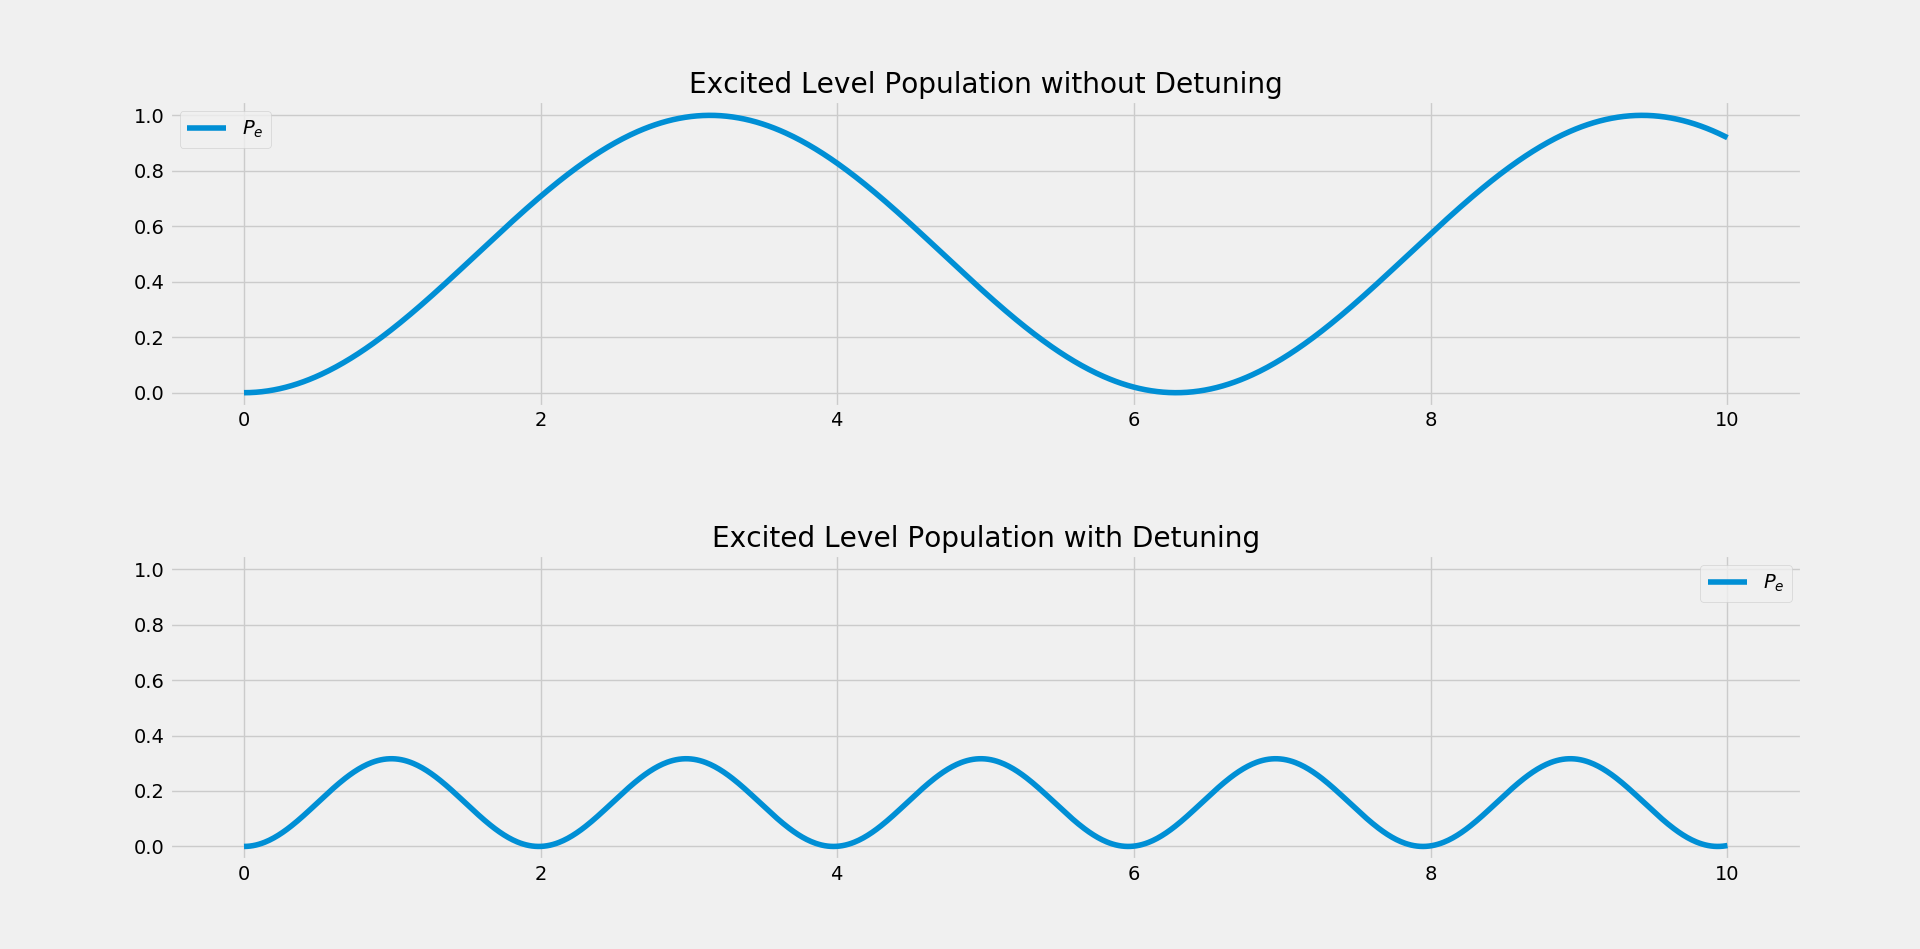
\includegraphics[width=1.0\columnwidth]{Rabi-Oscillations.png}
    \caption{Rabi oscillations of atom in a classical electromagnetic field. The top graph is without detuning $\Delta = 0$ and the bottom graph is with detuning $\Delta \ne 0$}
    \label{fig:rabi-oscillations}
\end{figure}
You can see without detuning the atom oscillates between ground and excited and there are two note able differences between the oscillations with and without detuning. With detuning the the atom doesn't reach the excited state, it does part of the way and then goes back down, this means you can't send simple. This means that if you want  to get to the excited states you need to send a pulse with exactly the same frequency as the atom. The other difference is that with detuning the oscillations are more rapid.

We can take everything we got so far and construct a pulse that will take the ground state into the excited state. First the pulse must have the same frequency as for the energy level difference in the atom. If the total time of the pulse is T then the amplitude of the pulse should be one so that the Rabi oscillations just reach the excited states. We can put this into an equation
\[
    P_e(T) = 1 = (1 - \cos (\Omega_0 T))
\]
And the solutions are
\[
    \Omega_0 = \frac{\pi k}{T} \quad \text{for} \quad k = 1, 2, 3, \dots
\]
Where $k$ corresponds to the amount of oscillations between the ground and excited states. Ideally the atom would go directly to the excited state without doing all that back and forth stuff.

Putting it all together, for a two level atom with energy difference between the levels of $\hbar \omega_0$, and a pulse with duration $T$, the pulse you need to send to get from the ground state to the excited state is
\[
    \boxed{\Omega(t) = \frac{\pi}{T} e^{i \omega_0 t}}
\]
Where the real and imaginary parts correspond the sin and cos waves we send to the atom(or I and Q pulses if you prefer). Writing them explicitly we get
\[
    \boxed{\Omega_I (t) = \frac{\pi }{T} \sin (\omega_0 t)} \quad \text{and} \quad \boxed{\Omega_Q (t) = \frac{\pi}{T} \cos (\omega_0 t)}
\]
We can actually check using the simulation we made in chapter \ref{chap:optimal} and see that yes! These pulses lead to the qubit going from the ground to excited states, amazing!

There is actually a more general result about \textit{$\pi$-pulses} we can see from here, we won't prove it but we can see it works. Any pulse, doesn't has to be a sinusoidal, that satisfies
\[
    \int_0^T \Omega(t) dt = \pi
\]
Would take the ground state atom to the excited state. You can use a something like a Gaussian or some other weird pulse that satisfies it and they will all work. We can see that indeed, the pulse we made does satisfy it.

There are actually much more examples we can find analytical solutions for, even for a 3-level system coupled with a cavity but we won't touch on them here, they are much more complicated, although they are definitely possible to calculate analytically. What we got is the super important result of called the Rabi oscillations and it's important to understand what people mean when they talk about them.

\newpage
\section{Another Method: Computational Graphs}
In the optimal control section, in essence, we try to minimize the cost of many many variables, this is a similar problem that to teaching neural networks and machine learning, we might be able to borrow some tricks and method they use to solve our problem.

Instead of thinking of a cost function as just a function, we can treat it as a \textit{computational graph}. We'll discuss briefly about what's a computational graph and how can we implement GRAPE using one. We won't go in depth as we did in the chapter on optimal control, it's only a general overview meant to show an alternative method. Let's start by defining a computational graph\footnote{Of course, graph theory is an entire field of mathematics by itself and we can't really give a rigorous definition, but more of an intuitive explanation}.
% TODO: Add imagry of a computational graph
\subsection{What are Computational Graphs}
A computational graph consists of nodes and connection between them, a node can be one of one of three things
\begin{itemize}
    \item \textbf{Operations}, the operation takes a list of numbers from other nodes and outputs another list of numbers(doesn't need to be of same size) % TODO: Change wording of this line
    \item \textbf{Parameters}, these are, as the name suggests, the parameters of the graph and can be used by the operations.
    \item \textbf{Variables}, these are the variables that of the graph, and they too can be used by the operators of the graph
\end{itemize}
The graph starts as the variables, goes through some operations that use parameters and gives out some resualt. Let's take a look at a simple example
% TODO: Maybe make my own image so all the images have the same theme
\begin{figure}[H]
    \centering
    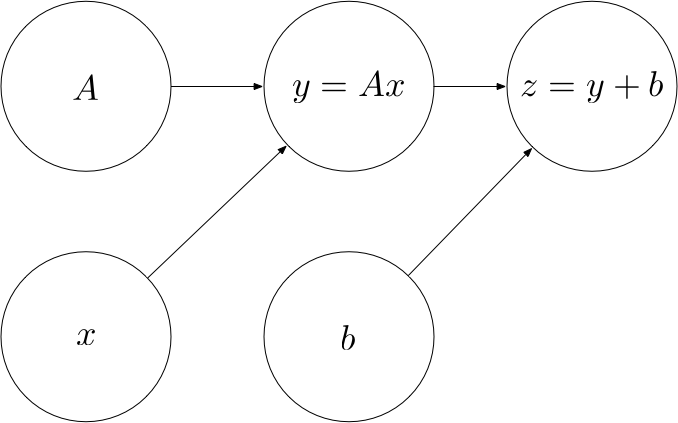
\includegraphics[width=0.4\columnwidth]{Example-comp-graph.png} %TODO: Change image to one with L I R markings
    \caption{Example of a basic computational graph}
    \label{fig:example-computational-graph}
\end{figure}

Here, $x$ is the variable, $A$ and $b$ are the parameters, and $y$ and $z$ are the operators. The function that this graph represents is $y = a \cdot e^{x}$. For now it properly seems overkill to use the graph to represent that simple of a function but in the next two sections you'll see the magic of the computational graph, in terms of thinking about the gradient.

\subsection{Back-Propagation}
This is the magic of the computational graph, calculating the gradient of the cost function by back-propagating the derivatives to the initial variables. The idea is simple, instead of trying to directly calculating the gradient, we calculate the derivative of node by the previous node, and relate the cost function to the variables by the chain rule. What does that mean, let's show an example.

Let's say we have a simple comutational graph that looks like
\[x \rightarrow L_1 \rightarrow L_2 \rightarrow L_3 \rightarrow y\] % TODO: Maybe change this to a graphical image
and we want to calculate the derivative, $\frac{\partial y}{\partial x}$. Instead of calculating the derivative directly, we can back-propagagte the derivatie as
\[\frac{\partial y}{\partial x} = \frac{\partial y}{\partial L_3} \cdot \frac{\partial L_3}{\partial L_2} \cdot \frac{\partial L_2}{\partial L_1} \cdot \frac{\partial L_1}{\partial x} \cdot \frac{\partial y}{\partial x}\]
luckily for us each operation is very simple so each derivative is simple as well.
% TODO: Maybe add an example like the one before(or even use the same example)
\subsection{GRAPE in a Computational Graph}
Now we can finally implement grape as a computational graph, we'll consider the simplest case of GRAPE, no constraints, only the original definition(see equations \ref{eq:fidelity_sim}, \ref{eq:U_def_prod} and \ref{eq:hamiltonianl_form})\footnote{This is assuming only one drive hamiltonian, for more drives the only difference is adding $\epsilon'_k H'_d$ and so on for each drive} %TODO: Change wording of footnote and add explenation where the function comes from
\[
    F(\vec{\epsilon}) = \abs{\bra{\psi_{target}} \prod_{i=0}^N e^{-i \cdot \delta t (H_0 + \epsilon_k H_d)} \ket{\psi_{initial}}}^2
\]
In this case, $\vec{\epsilon}$ is the variable, $H_0$, $-i \cdot \delta t$, $\bra{\psi_{target}}$ and $\ket{\psi_{initial}}$ are the parameters. They relate through the operators and everything can be displayed as the following graph\footnote{Simplifying for 3 time steps, to add more time steps is pretty straight forward}
% TODO: Add the graph
\begin{center}
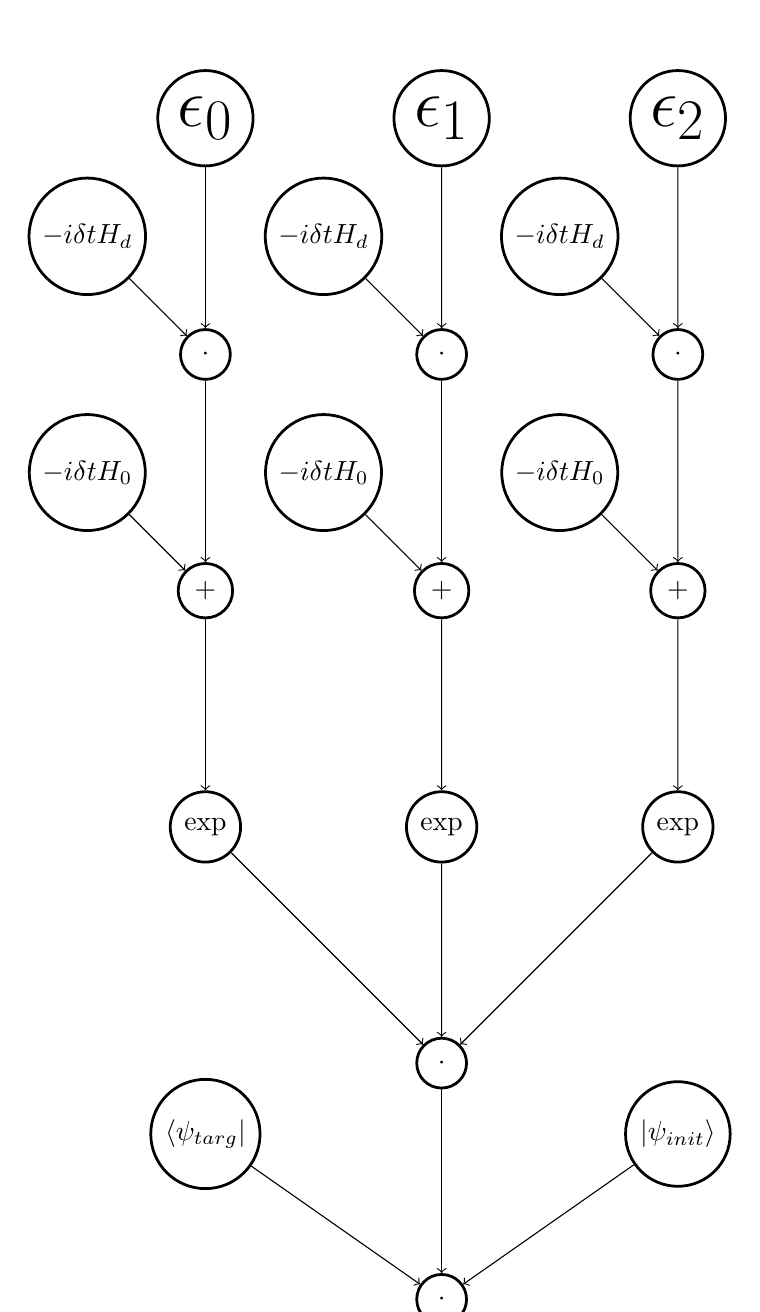
\begin{tikzpicture}[scale=3]
\renewcommand*{\VertexLineWidth}{1pt}%vertex thickness
\renewcommand*{\EdgeLineWidth}{1pt}% edge thickness
\GraphInit[vstyle=Normal]
% Variables
\Vertex[L={\Huge $\epsilon_0$}, x=0,y=5]{e0}
\Vertex[L={\Huge $\epsilon_1$},x=1,y=5]{e1}
\Vertex[L={\Huge $\epsilon_2$},x=2,y=5]{e2}

\Vertex[L=$-i \delta t H_d$,x=-0.5,y=4.5]{idt00}
\Vertex[L=$-i \delta t H_d$,x=0.5,y=4.5]{idt01}
\Vertex[L=$-i \delta t H_d$,x=1.5,y=4.5]{idt02}
% L1
\Vertex[L=$\cdot$,x=0,y=4]{L10}
\Vertex[L=$\cdot$,x=1,y=4]{L11}
\Vertex[L=$\cdot$,x=2,y=4]{L12}

\Vertex[L=$-i \delta t H_0$,x=-0.5,y=3.5]{idt10}
\Vertex[L=$-i \delta t H_0$,x=0.5,y=3.5]{idt11}
\Vertex[L=$-i \delta t H_0$,x=1.5,y=3.5]{idt12}
% L2
\Vertex[L=$+$,x=0,y=3]{L20}
\Vertex[L=$+$,x=1,y=3]{L21}
\Vertex[L=$+$,x=2,y=3]{L22}
% L3
\Vertex[L=$\exp$,x=0,y=2]{L30}
\Vertex[L=$\exp$,x=1,y=2]{L31}
\Vertex[L=$\exp$,x=2,y=2]{L32}
% L4
\Vertex[L=$\cdot$,x=1,y=1]{L4}

\Vertex[L=$\ket{\psi_{init}}$,x=2,y=0.7]{psii}
\Vertex[L=$\bra{\psi_{targ}}$,x=0,y=0.7]{psit}
% C
\Vertex[L=$\cdot$,x=1,y=0]{C}

%%%%%%%%%%%%%%%%%%%%%%%%%%%%%%
\draw [->] (e0) edge (L10);
\draw [->] (e1) edge (L11);
\draw [->] (e2) edge (L12);
\draw [->] (idt00) edge (L10);
\draw [->] (idt01) edge (L11);
\draw [->] (idt02) edge (L12);

\draw [->] (L10) edge (L20);
\draw [->] (L11) edge (L21);
\draw [->] (L12) edge (L22);
\draw [->] (idt10) edge (L20);
\draw [->] (idt11) edge (L21);
\draw [->] (idt12) edge (L22);

\draw [->] (L20) edge (L30);
\draw [->] (L21) edge (L31);
\draw [->] (L22) edge (L32);

\draw [->] (L30) edge (L4);
\draw [->] (L31) edge (L4);
\draw [->] (L32) edge (L4);

\draw [->] (L4) edge (C);
\draw [->] (psii) edge (C);
\draw [->] (psit) edge (C);

\end{tikzpicture}
\end{center}
The layers are as follows
% TODO: Add the layers
\begin{align*}
    L_1^k &= -i \delta t H_d \epsilon_k \\
    L_2^k &= -i\delta t H_0 + L_1^k \\
    L_3^k &= e^{L_2^k} \\
    L_4 &= \prod_{k=0}^N L_3^k \\
    C &= \bra{\psi_{target}} L_4 \ket{\psi_{initial}}
\end{align*}

And the derivatives are calculated rather easily as
% TODO: Add derivarives
\begin{align*}
    \frac{\partial L_1^k}{\partial \epsilon_k} &= -i \delta t H_d\\
    \frac{\partial L_2^k}{\partial L_1^k} &= 1 \\
    \frac{\partial L_3^k}{\partial L_2^k} &= e^{L_2^k} \\
    \frac{\partial L_4}{\partial L_3^k} &= \prod_{i \ne k} L_3^i \\
    \downarrow \\
    \frac{\partial C}{\partial \epsilon_k} &= \bra{\psi_{target}}  \frac{\partial L_4}{\partial L_3^k}  \frac{\partial L_3^k}{\partial L_2^k} \frac{\partial L_2^k}{\partial L_1^k}  \frac{\partial L_1^k}{\partial \epsilon_k} \ket{\psi_{init}}
\end{align*}
It's important to note that $\frac{\partial L_1^i}{\partial \epsilon_j} = 0$ for $i \ne j$ so we didn't refer to those derivative(This is true for the derivative between any two layers).

We now everything we need to implement GRAPE as a computational graph, and we can use a library, such as google's tensorflow, to find the optimal pulse.

\newpage
\section{Quantizing Electric Circuit and the Josephson Junction} \label{appen:LC}
Throughout the project, I mentioned several times that the physical implementation of the qubit is not  the subject of the project and ignored it. It would be a crime no to at least give a simple explanation of the implementation of the qubit, especially since we dedicated and entire section(section \ref{sec:DRAG}) to the problem with our physical implementation. In this appendix I will try to give a simple explanation of  the qubit as a quantum LC circuit, using the  tools we got when we quantized the electromagnetic field.

This appendix is here for two reasons. The first we already mentioned, to gain some insights on how the qubit is implemented physically. The second, less obvious reason, is to really drive home the point that Dirac's method for Canonical quantization can be applied to any oscillating phenomena, from mechanical oscillator, to the electromagnetic field and even an LC circuit as we'll show here. This shows how amazing is the Dirac formalism is and how general an applicable it is.

\subsection{Quantizing the LC Circuit}
Before we look at the actual qubit, lets first quantize the LC circuit. The LC circuit is constructed by connecting a capacitor with capacitance $C$ to a coil with inductance $L$, hence the name, \textit{LC}. Drawing it in a diagram is as shown
\begin{figure}[H]
    \centering
    % TODO: Change image to one with marking of the magnetic inductance field and the  electric capacitance field
    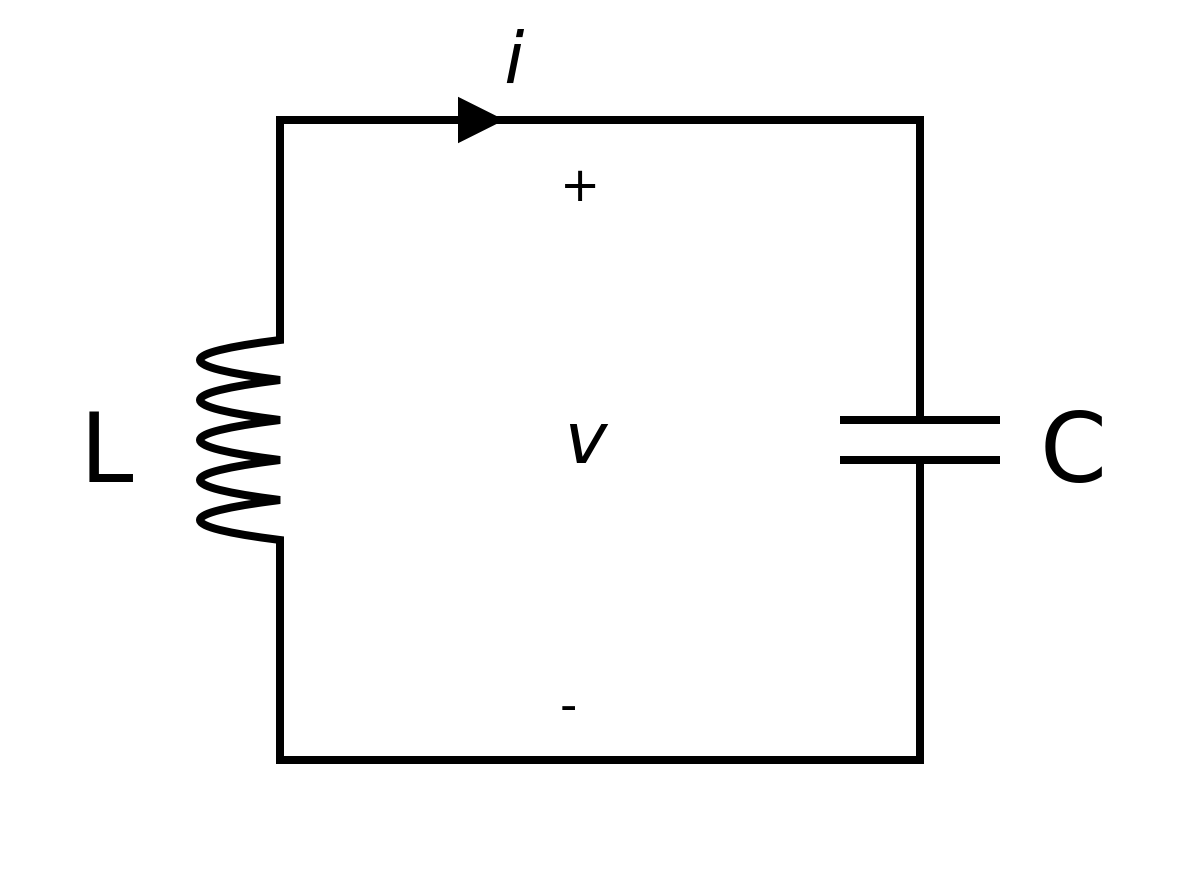
\includegraphics[width=0.5\columnwidth]{LC-circuit.png}
    \caption{The LC circuit} 
    \label{fig:LC-circuit}
\end{figure}

To begin the quantization we first need choose a pair of canonically conjugate variables that represents the state of the system. The most obvious pair of variables would be the voltage $V$ and the current $I$, but turns out they are not canonically conjugate variables, instead, we'll choose the charge of the capacitor $q$ and the inductor's magnetic flux $\phi$ to be the variables. 
% TODO: Maybe check the V and I are not canonically conjugate
Let's check that they are really canonically conjugate. The energy(and therefore, the Hamiltonian) of the capacitor's electric field is given by
\[
    H_C = \frac{q^2}{2C}
\]
and the energy of the magnetic field stored in the inductor is given by
\[
    H_L = \frac{\phi^2}{2L}
\]
Now we can sum these two donations to the Hamiltonian and get that the Hamiltonian of the LC circuit is
\[
    H_{LC}(q, \phi) = \frac{\phi^2}{2L} + \frac{q^2}{2C}
\]
Lets now write the Hamilton equations of motion and see if $q$ and $\phi$ are actually canonically conjugate
\begin{align}
    &\dot{q} = \quad \frac{\partial H_{LC}}{\partial \phi} = \quad \frac{\phi}{L} = \quad I \label{eq:def-current}\\
    &\dot{\phi} = -\frac{\partial H_{LC}}{\partial q} = -\frac{q}{C} = -V \label{eq:def-potential}
\end{align}
These equation are current since \ref{eq:def-current} is the definition of current and \ref{eq:def-potential} is the definition of potential. We have no proven that $q$ and $\phi$ are canonically conjugate variables and can go on to quantize them.

To quantize these variables we simply need to replace them with operators
\begin{align*}
    q \rightarrow \hat{q} \\
    \phi \rightarrow \hat{\phi}
\end{align*}
satisfying the commutation relation
\[
    [\hat{q}, \hat{\phi}] = i\hbar
\]
as always with quantum harmonic oscillator we'll define annihilation and creation operators
\begin{align*}
    &\hat{a} = \frac{\hat{q}}{q_0} + i\frac{\hat{\phi}}{\phi_0} \\
    &\hat{a}^\dag = \frac{\hat{q}}{q_0} - i\frac{\hat{\phi}}{\phi_0}
\end{align*}
where
\begin{align*}
    &q_0^2 = 2\hbar\sqrt{\frac{C}{L}} \\
    &\phi_0^2 = 2\hbar\sqrt{\frac{L}{C}}
\end{align*}
% TODO: Maybe don't skip the basic algebra
After some algebra magic we can get the expression of the Hamiltonian
\[
    \hat{H}_{LC} = \hbar \omega (\hat{a}^\dag \hat{a} + \frac{1}{2}) \quad \text{with} \quad \omega = \frac{1}{\sqrt{LC}}
\]
This is the good old expression for the Hamiltonian of a quantum harmonic oscillator and we can treat at as we did with any other quantum harmonic oscillator, getting all the number states and observable of the system from the creation and annihilation operators.

\subsection{Artificial Atoms - The Josephson Effect}
The problem with the simple quantum LC circuit is that it's energy levels are \textit{linear}. By linear, I mean that the difference in energy between two neighboring levels is the same for every level, $E_{n + 1} - E_n = \hbar \omega$ for all $n$. This is a problem since we want to treat it as a two level system but if we send a pulse with $\hbar \omega$ energy we want it to affect only the lower two levels but since the energy difference between the levels is the same for all levels, sending such a pulse would also excite the higher levels and we don't want that.
% TODO: Add energy level diagrams
We want to introduce \textit{un-linearity} to the levels, so still $E_1 - E_0 = \hbar \omega_{01} $ but $E_2 - E_1 = \hbar \omega_{12}$, $E_3 - E_2 = \hbar \omega_{23}$ and so on, where $\omega_{n\ n+1} \ne \omega_{01}$. This way if the system is only populated at one of the lower two levels and we send a pulse with energy $\hbar \omega$, the only levels affected are the lower two and not the higher ones\footnote{This is obviously an ideal case, as we seen in section \ref{sec:DRAG} about DRAG, this is not always the case and we need to add correction to make it work}.

To create these a-linearities we can use the \textbf{\textit{Josephson Junction}}, a Josephson junction is simply a cut in the wire, a very(very) thin cut, the two pieces of wire are around 10nm apart. The Josephson junction replaces that inductor in the LC circuit. A full description of the Josephson junction is way out of the scope of this appendix but we'll give a brief overview of how it works. The Josephson Junction in a circuit diagram is drawn as a little $x$, and the circuit diagram of the LC circuit with it is
\begin{figure}[H]
    \centering
    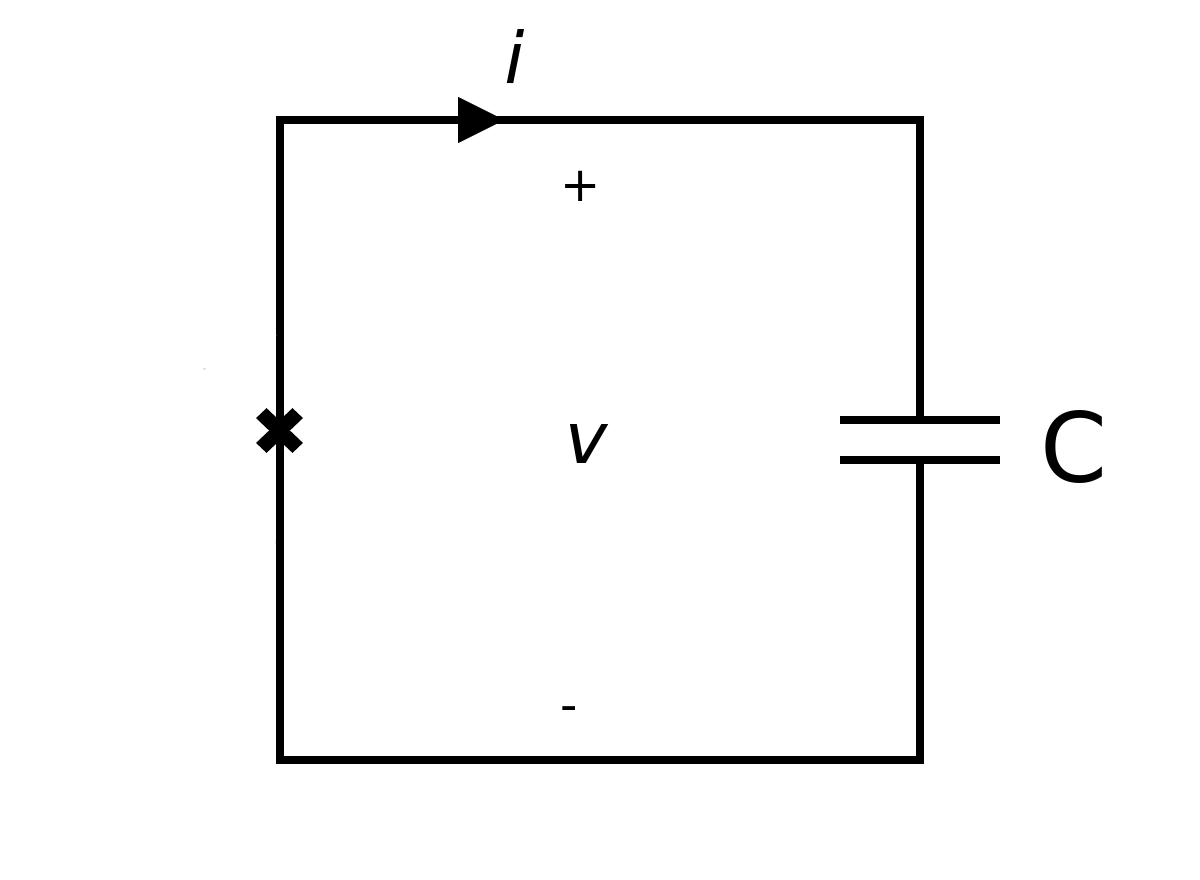
\includegraphics[width=0.5\columnwidth]{LC-circuit-josephson.png}
    \caption{The LC circuit with a Josephson junction} 
    \label{fig:LC-circuit-Josephson}
\end{figure}
And the effect of adding a Josephson junction is\footnote{An intuition for this will be given shortly} replacing the Hamiltonian of the inductor $\frac{\phi^2}{2L}$ with $E_j \cos (\frac{2e}{\hbar} \phi)$.
\[
    \hat{H}_{Josephson} = \frac{\hat{q}^2}{2C} + E_j \cos (\frac{2e}{\hbar} \phi)
\]
This does exactly what we want, for the first level we can approximate the cosine as a parabola and get $E_1 - E_0 = \hbar \omega_{01}$ but since the cosine diverges from the parabola after that the difference between the energy levels lessens and lessens between each pair of higher levels. Here's a visual representation of the energy level of the LC circuit with the Josephson junction
\begin{figure}[H]
    \centering
    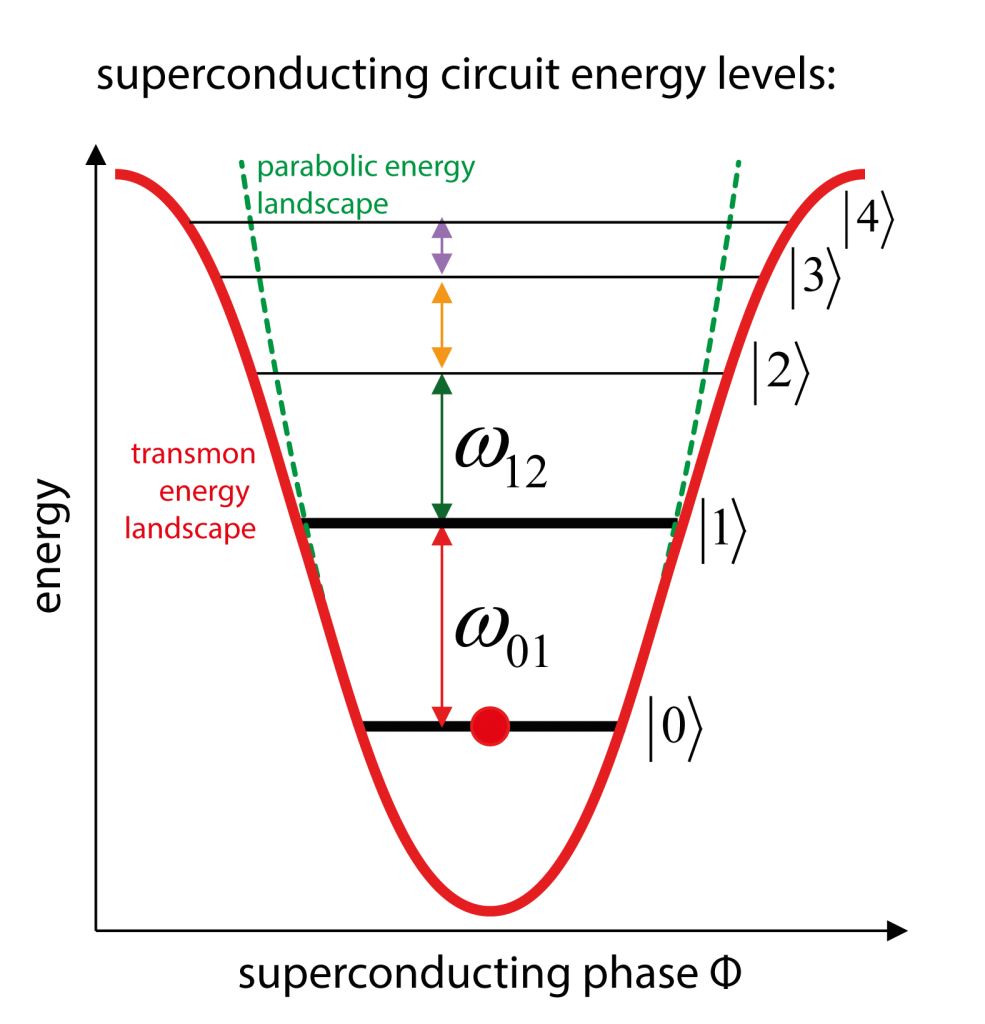
\includegraphics[width=0.5\columnwidth]{josephson-energy-levels.png}
    \caption{Potential of the circuit as a function of the superconducting phase, and the non-linear energy levels of the Josephson junction} 
    \label{fig:Josephson-energy-levels}
\end{figure}
While I won't give an exact explanation for why this is the resulting Hamiltonian, we can still get a nice intuition for it by a rather simple calculation. We can treat the Josephson junction as a potential barrier, and calculate the wave function on both sides of the wire.

We'll call the wave function on one side of the junction $\psi_1$ and on the other side $\psi_2$, their dynamics are determined by the coupled shr\"{o}dinger equations:
\begin{align*}
    &i\hbar\frac{\partial \psi_1}{\partial t} = \mu_1 \psi_1 + K \psi_2 \\
    &i\hbar\frac{\partial \psi_2}{\partial t} = \mu_2 \psi_2 + K \psi_1 
\end{align*}
Where $K$ is the coupling across the barrier and $\mu_{1/2}$ are the lowest energy states of each wave function. We'll "guess" solutions of the form
\[
    \psi_{1/2} = \sqrt{n_{1/2}}e^{i\theta_{1/2}}
\]
Yielding the two equations
\begin{align*}
    &\hbar \frac{\partial n_1}{\partial t} = - \hbar \frac{\partial n_2}{\partial t} = 2K \sqrt{n_1 n_2} \sin (\theta_2 - \theta_1) \\
    -&\hbar \frac{\partial (\theta_2 - \theta_1)}{\partial t} = \mu_2 - \mu_1
\end{align*}
$n_{1/2}$ are the density of cooper pairs, and by definition of the current, the current is $\frac{\partial n_1}{\partial t}$. When voltage is applied the energy levels shift as $\mu_2 - \mu_1 = 2eV$. Finally to make the equations shorter we'll write $I_0 = 2K\sqrt{n_1 n_2}$ and $\delta = \theta_2 - \theta_1$. The equations now become
\begin{align*}
    &I = I_0 \sin \delta \\
    &\frac{\partial \delta}{\partial t} = \frac{2eV}{\hbar}
\end{align*}
% If we apply constant voltage(i.e. DC voltage) then we get the simple solution that
% \begin{align*}
%     &\delta = \frac{2eV_0}{\hbar} + \delta_0 \\
%     &I = I_0 \sin (\frac{2eV_0}{\hbar} + \delta_0)
% \end{align*}
We can now calculate the electric power(which is the derivative of the energy) from the classical equation
\[
    \frac{\partial E}{\partial t} = P = I V = (I_0 \sin \delta) \cdot (\frac{\hbar}{2e} \frac{\partial \delta}{\partial t}) = -\frac{I_0 \hbar}{2e} \frac{\partial \cos \delta}{\partial t}
\]
Integrating over time, we get that the expression for the energy is
\[
    E = -\frac{I_0 \hbar}{2e} \cos \delta
\]
If we define $E_j -\frac{I_0 \hbar}{2e}$ and write $\delta \rightarrow \hat{\phi}$ and replace the energy with the Hamiltonian, we get
\[
    \hat{H}_{Josephson} = E_j \cos \hat{\phi}
\]
just as we've written earlier.

This is not the best treatment of the Josephson junction but it's a rough idea of the explanation. This expression gives us the a-linearities we want to get to implement the qubit.

% Since we know from classical physics that the inductance of a coil and the current going through it are related(linearly), $\phi \propto I$, the expression we've shown for the Hamiltonian of the Josephson junction is simply that as we got from here. Even though this is the correct way to treat the Josephson junction, it still gives us intuition for why the expression for the Hamiltonian is correct and in fact the Josephson junction does create a-linearities.


% TODO: Add content, see coursera course first lesson last video

% \newpage
% %Examples of mixers and couplers
% \section{Couplers and Mixers(?)} \label{appen:Mixers} % Maybe I'll get rid of this section entierly
% Our goal here is to understand some ways you could physically implement some of the components in chapter \ref{chap:FPGA}, there are a lot of ways to implement each component but we're going to look at only a few. First we'll look into how would you implement a mixer, and then we'll see how would you implement a coupler(to make a phase difference).
% \subsection{Single-Ended Diode Mixer}
% \subsection{Single-Ended FET Mixer}
% \subsection{Ring Modulator}
% \subsection{Branch-Line Quadrature(90\degree) Coupler}
% \subsection{Rat-Race Coupler}

% \newpage
% \section{Codes} \label{appen:Codes}
% All the codes are available online at https://github.com/DanielCohenHillel/Controlling-a-Superconducting-Quantum-Computer
% \subsection{IQ Mixer Optimization}
% \subsection{GRAPE}
% \subsection{Transmon-Cavity GRAPE}

% \newpage
% \section{Optimization Algorithms(?)} \label{appen:opt}
% \subsection{fmin}
% \subsection{L-BFGS-B}

\newpage
% TODO: Properly need to change this completely :(
% \begin{thebibliography}{9}  % TODO: Format the bibliography correctly
%     \bibitem{Phillip}
%         Controlling Error Correctable Bosonic Qubits
%     \bibitem{Phillip}
%         Introductory Quantum Optics
%     \bibitem{Quantum Computing and Quantum Information}
%         Quantum Computing and Quantum Information
%     \bibitem{Microwave Engineering}
%         Microwave Engineering
%     \bibitem{Quantum Computing: An Applied Approch}
%         Quantum Computing: An Applied Approch
%     \bibitem{QuTIP} 
%         J. R. Johansson, P. D. Nation, and F. Nori: "QuTiP 2: A Python framework for the dynamics of open quantum systems.", Comp. Phys. Comm. 184, 1234 (2013) [DOI: 10.1016/j.cpc.2012.11.019].
% \end{thebibliography}

\end{document}


